% ---- ETD Document Class and Useful Packages ---- %
\documentclass{ucetd}
\usepackage{subfigure,epsfig,amsfonts}
%%\usepackage{natbib}  % AKK: original natbib include
\usepackage[square,sort,comma,numbers]{natbib}
\usepackage{amsmath}
\usepackage{amssymb}
\usepackage{amsthm}

% custom stuff (for ATLAS, figures, etc)
\usepackage{multirow}
\usepackage[multidot]{grffile}
\usepackage{graphicx}
\usepackage{dcolumn}
\usepackage{longtable}
\usepackage{ctable}
\usepackage{verbatim}
\usepackage{enumitem}
\usepackage{url}
%\usepackage[subfigure]{tocloft}

% hyperlinks
\usepackage{hyperref}
\hypersetup{linktocpage}


\usepackage{atlasphysics}
/home/antonk/SupportingDocument/WZDefinitions.tex
% Shorthand for \phantom to use in tables
\newcommand{\pho}{\phantom{0}}
\newcommand{\bslash}{\ensuremath{\backslash}}
% Our macros and units
\usepackage{macross}

% Shortcuts
\newcommand{\tbu}{{\color{red}TO BE UPDATED }}
\def\Wpmmn{\ensuremath{W^\pm \rightarrow \mu\nu}}
\def\Wpmen{\ensuremath{W^\pm \rightarrow e\nu}}
\newcommand{\lumioldtr}{\ensuremath{35\,\mathrm{pb}^{-1}}}

%% Use these commands to set biographic information for the title page:
\title{
Measurement of differential inclusive W boson production and decay cross sections in the muon channel using the ATLAS Detector
}
\author{Anton Kapliy}
\department{Physics}
\division{Physical Sciences}
\degree{Doctor of Philosophy}
\date{December 2013}

%% Use these commands to set a dedication and epigraph text
\dedication{Dedication Text}
%\epigraph{Before I came here I was confused about this subject. Having listened to your lecture I am still confused. But on a higher level. \\ Enrico Fermi}
%\epigraph{ What I am going to tell you about is what we teach our physics students in the third or fourth year of graduate school... It is my task to convince you not to turn away because you don't understand it. You see, my physics students don't understand it... That is because I don't understand it. Nobody does. \\ Richard Feynman }
\epigraph{ \textit{We have a closed circle of consistency here: the laws of physics produce complex systems, and these complex systems lead to consciousness, which then produces mathematics, which can then encode in a succinct and inspiring way the very underlying laws of physics that gave rise to it.} }
\epigraphattr{ Roger Penrose }

\begin{document}

%% Basic setup commands
% If you don't want a title page comment out the next line and uncomment the line after it:
\maketitle
%\omittitle

% These lines can be commented out to disable the copyright/dedication/epigraph pages
\makecopyright

% \makededication
\makeepigraph


%% Make the various tables of contents
\tableofcontents
\listoffigures
\listoftables

\acknowledgments
% Enter Acknowledgements here
% acknowledgements

First and foremost, I would like to thank my adviser Mel Shochet. With Mel's guidance, support, and funding, I have worked on several exciting projects at Chicago: from the software simulations of the FastTracker trigger, to the hardware and firmware development of a high-speed transceiver circuit board, to a precision-electroweak analysis measuring the differential cross-sections of the \Wpm\ bosons. Mel combines several decades of experience in all facets of high energy physics research with an amazing intuition: whenever I approached him with a problem, I always received a well-thought advice that was right on the money.

In addition to Mel, I am grateful to David Biron, Yau Wah, and Liantao Wang, who agreed to serve on my Ph.D. committee.

I thank my colleagues at CERN and at various European universities, including Massimiliano Bellomo, Jan Kretzschmar, Adrian Lewis, and many others. This analysis was a collective effort by the entire W/Z-inclusive team.

The high-energy physics group at Chicago has been a valuable asset since my first day at the university. From private discussions, to seminars and conferences, I have learned a lot from the professors and other group members at Chicago and have benefited greatly from a friendly and nurturing environment.

Several post-docs shared their expertise and wisdom, including John Alison, Antonio Boveia, Erik Brubaker, Bjoern Penning, Lauren Tompkins, Joe Tuggle, Guido Volpi, and Kohei Yorita. Peter Onyisi provided so much input at all stages of this analysis that he qualified as the co-author.

A number of HEP students shared with me the joys and challenges of graduate-student life, including Yangyang Cheng, Tudor Costin, Jeff Dandoy, Eric Feng, Karol Krizka, Shawn Kwang, Ho Ling Li, Sam Meehan, Constantinos Melachrinos, Sasha Paramonov, Jian Tang, Jordan Webster, Daping Weng, and Zihao Zhang.

The computing resources available at Chicago allowed me to run the analysis through multiple iterations in a quick and efficient manner. My thanks go to Rob Gardner and his team: Lincoln Bryant, David Champion, Marco Mambelli, Aaron van Meerten, Charles Waldman, Ilija Vukotic, and Nathan Yehle.

Mary Heinz provided first-class IT support throughout the years. She often went above and beyond the call of duty - from quick responses to my weekend pleas to reboot a server that went down, to setting up obscure Linux device drivers.

For a couple of years, I worked in the electronics shop side-by-side with Mircea Bogdan, Jean-Francois Genat, Harold Sanders, and Mark Zaskowski. Fukun Tang and I had a lot of fun designing and building nearly three hundred data transmission cards and shared many conversations in the process.

In my first year at Chicago, I was a teaching assistant for the introductory physics classes and received much-appreciated guidance from Van Bistrow and Stuart Gazes. Autym Henderson, Nobuko McNeill, and Aspasia Sotir-Plutis helped me navigate through the bureaucratic rules at the university and ensured that I always got paid on time and received reimbursement for my travel expenses.

My parents Sergey and Liubov, my brother Denis, and my extended family in Russia and China have provided unyielding love and support throughout graduate school. My gratitude to them is boundless.

I met Meng Ning in a physics lab in KPTC during my first year of graduate school. Fast-forward to today, and we are about to celebrate our fifth wedding anniversary. Meng has always been there for me, and I am very excited as the two of us, along with our cats, are opening a new page in our lives in Boston.


\abstract
% Enter Abstract here
% abstract

% The distributions for the main observables are compared to Monte Carlo simulations. 
% , integrated over transverse momentum

This thesis presents the measurement of \Wmn\ inclusive cross-sections based on proton-proton collisions at $\sqrt{s}=7\tev$ with an integrated luminosity of \lumitr, collected with the ATLAS detector in 2011. The charge-dependent $W^{\pm}$ differential cross-sections are provided in bins of muon pseudorapidity as well as double differentially in muon pseudorapidity and muon transverse momentum. The data are also presented as integrated cross-sections, in the fiducial region of the measurement and extrapolated to full phase space. Results are compared to predictions computed at NNLO QCD for different NNLO sets of parton distribution functions. The \Wmn\ cross-sections are combined with complementary measurements in \Wen, \Zmm, and \Zee\ channels and used in a dedicated NNLO QCD analysis to obtain new constraints on the parton distributions in the proton.


\mainmatter
% Main body of text follows

%1
\chapter{Introduction}
\label{chap:intro}
% introduction, thesis outline

\section{Executive Summary}

The Large Hadron Collider (LHC) is the world's largest and highest-energy particle accelerator. Located on the border of Switzerland and France, it collides two energetic proton beams, creating sub-atomic particles that are hard to produce in other ways. Among these are the positive and negative \Wboson\ bosons, which are the mediators of the weak nuclear force. Although \Wboson\ bosons decay quickly before reaching the detector, their decay products can often be identified and measured experimentally. This thesis measures the propensity of \Wboson\ decay products to appear at different angles or energies, i.e. differential cross-sections, which provides a precise test of perturbative Quantum Chromodynamics (QCD) and a validation of theoretical predictions at next-to-next-to-leading order (NNLO). These measurements also provide valuable information about the structure of the proton, which is not calculable from the first principles.

The analysis uses the full 2011 dataset collected from the ATLAS experiment, one of two general-purpose detectors at the LHC. The ATLAS detector is designed to measure the energy and direction of the particles that emanate from the collision point. This thesis focuses on the \Wpmmn\ decay channel, where the muon is detected explicitly in the inner tracker and muon chambers, while the non-interacting neutrino is inferred through the presence of momentum imbalance in the detector. A complementary measurement in the \Wpmen\ channel was simultaneously performed by a different team and combined with the results obtained in this thesis.

The measurement is considered ``inclusive'' in the sense that it does not distinguish between final states with different numbers of jets - collimated sprays of hadrons that may be produced along with the \Wboson\ boson. These multi-jet final states are explored in a separate $W+jets$ analysis~\cite{Aad:2012en}.

\section{Thesis Outline}

During 2011, the LHC operated at the center-of-mass energy of $7\tev$, about half of its maximum design energy, but substantially higher than the $2\tev$ accessible in the recently completed Tevatron program at Fermilab. The ATLAS and CMS collaborations previously published analyses of the inclusive \Wboson\ production cross-sections at $7\tev$ using the 2010 dataset, with an integrated luminosity of \lumioldtr~\cite{Aad:2011dm,CMS:2011aa}. This thesis extends those measurements to the full 2011 sample with \lumitr, a more than 100-fold increase in integrated luminosity. The increased statistics along with improved understanding of the detector resulted in a significant decrease in experimental measurement uncertainties from 2\% to 1\% in the integrated and single-differential (angular variable) cross-sections. In addition, this thesis provides the first measurement of the double-differential cross-sections binned in both the angular variable and the transverse momentum of the muon.

Chapter~\ref{chap:method} explains the methodology for cross-section calculation and defines the phase space and binning used in each part of the measurement. Chapter~\ref{chap:det} introduces the LHC and the key components of the ATLAS detector. Chapter~\ref{chap:th} describes the theory behind \Wboson\ boson production at hadron colliders and outlines the process of obtaining theoretical predictions. Chapter~\ref{chap:mc} describes the data and Monte-Carlo samples used in the analysis. Chapter~\ref{chap:perf} focuses on the reconstruction performance and data-driven corrections for detector defects.

Chapter~\ref{chap:evt} describes experimental selection cuts and shows various kinematic distributions of the selected events. Chapter~\ref{chap:bg} reviews the backgrounds to the measurement and estimates their composition and uncertainty. Chapter~\ref{chap:unc} summarizes all experimental uncertainties for the integrated, single, and double-differential measurements. Chapter~\ref{chap:res} contains the numerical results of the analysis, comparisons with theory predictions, and newly-derived constraints on the parton distribution functions.

Chapter~\ref{chap:conc} summarizes the measurement and draws conclusions.


%2
\chapter{Methodology for Cross-Section Calculation}
\label{chap:method}
% method
\def\A{\ensuremath{A}}
\def\E{\ensuremath{E}}
\def\C{\ensuremath{C}}

\def\AW{\ensuremath{A_W}}
\def\EW{\ensuremath{E_W}}
\def\AZ{\ensuremath{A_Z}}
\def\EZ{\ensuremath{E_Z}}

\def\Wall{\ensuremath{\Wminus+\Wplus}}

The objective of this analysis is to measure the cross-section of \Wboson\ bosons decaying into a muon and a neutrino (in other words, the total production cross-section of the \Wboson, times its \Wmn\ branching ratio). The overall plan of attack can be summarized as follows:
\begin{itemize}
\item Starting with raw data events from the LHC, various cuts are applied to remove events that are inconsistent with the \Wmn\ process.
\item The surviving events are still contaminated with backgrounds that may mimic the experimental footprint of real \Wboson events. These backgrounds are estimated (from Monte-Carlo simulation or through data-driven methods) and subtracted from the pool of candidates.
\item Using \Wmn\ Monte-Carlo, the background-subtracted signal counts are adjusted for detector efficiency and resolution effects, and optionally extrapolated to a more inclusive phase space (for instance, to cover regions not directly instrumented by the detector). This procedure is called ``unfolding'' and produces a detector-independent measurement that can be directly compared against theoretical predictions.
\item The above steps are repeated several dozen times - once for each systematic variation - to assess the impact of these variations on the final measurement.
\end{itemize}

\section{The ATLAS Coordinate System}
The proton-proton interaction point serves as the pivot for the common coordinate system used at ATLAS. The z-axis runs along the beam line and the $x-y$ plane, which is perpendicular to the beam, defines the transverse plane. Transverse momentum $p_T$ is the projection of the particle momentum on the transverse plane, as illustrated in Fig.~\ref{fig:defetapt}(a). $\phi$ is the azimuthal angle in the transverse plane, while $\theta$ is the polar angle with respect to the beam axis. Transverse energy $E_T$ of a particle is defined as $E \cdot \sin \theta$. Missing transverse energy $\met$ quantifies the imbalance in the vectorial sum of transverse energies of all objects measured by the detector, which serves as a proxy for the $p_T$ of the particles that escape detection. Pseudorapidity $\eta$ is a monotonic transformation of the polar angle defined by the following formula:
$$\eta = -\log\biggl(\tan\frac{\theta}{2}\biggr)$$
The value of $\eta$ for different values of $\theta$ is illustrated in Fig.~\ref{fig:defetapt}(b).

\begin{figure}[phtb]
  \begin{center}
        \subfigure[Transverse momentum $p_T$]{%
          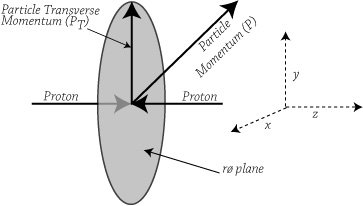
\includegraphics[width=0.44\textwidth]{method/fig/PT}
        }
        \subfigure[Pseudorapidity $\eta$]{%
          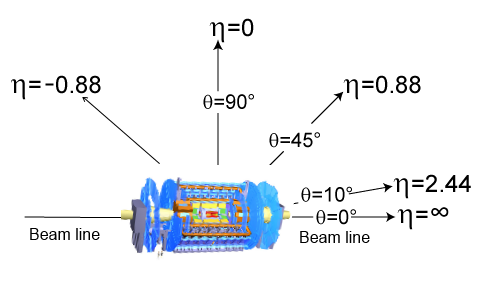
\includegraphics[width=0.44\textwidth]{method/fig/pseudorapidity}
        } 
 \caption{ Geometric illustration of the transverse momentum (left), polar angle and pseudorapidity (right). }
 \label{fig:defetapt}
 \end{center}
\end{figure}

\section{Integrated, Single and Double-Differential Measurements}
The \Wmn\ cross-sections are reported in three different binnings: integrated, single- and double-differential. All cross-sections are measured separately for \Wplus\ and \Wminus.

The integrated cross-section is unbinned and provides the production rate in the phase space covered by the detector, as well as in the full phase space. The single-differential cross-section is provided in bins of the absolute value of the muon pseudorapidity. The $|\eta|$ dependence of the cross-section provides valuable information about the proton structure, as elaborated in Sec.~\ref{chap:pdf_theory}. The double-differential cross-section further splits the measurement into bins of the transverse momentum of the muon in order to test whether the $p_T$ dependence of the cross-section is modeled properly by fixed-order theory calculations.

\section{Cross-Section Formula}
\label{sec:xsec_formula}
Mathematically, the cross-section can be derived from the following formula:
\begin{equation}
 \sigma \times BR =
 \frac{N - B}{\C \cdot \E \cdot \A \cdot L_{int}  \cdot \Gamma} \,,
\label{eq:WZxsec}
\end{equation}
where
\begin{itemize}
\item $N$ is the number of \Wboson\ candidate events in data,
\item $B$ is the number of background events,
\item $L_{int}$ is the integrated luminosity (total amount of collected data)
\item $\Gamma$ is the bin width. For differential measurements (but not integrated), the cross-sections are traditionally quoted per-unit of pseudorapidity or momentum, which allows for easier comparison of the values in variable-width bins.
\item \C\ is the factor used to correct for detector efficiency and resolution effects. It is derived from Monte-Carlo (MC below) and translates the cross-sections from ``reconstruction level'' to ``generator level'', which is independent of the specific features of the detector and can be defined in purely theoretical terms for a given fiducial phase space. 
    \begin{equation}
      \C = \frac{N_\mathrm{MC, rec, fiducial}}{N_\mathrm{MC, gen, fiducial}}\,. \label{eq:c}
    \end{equation}
 The \C\ factor does not perform any fiducial extrapolation: the same fiducial cuts ($p_T$, $\eta$, etc) are applied at the generator level as at the reconstruction level. However, it includes the effects of QED final state radiation, or FSR (radiation of additional photons off the muon) by correcting all muons down to a pre-FSR ``Born'' level.
\item \E\ is the factor used to perform a small theoretical extrapolation from $|\eta|<2.4$ to $|\eta|<2.5$. This is done for two reasons: to align \Wmn\ cross-sections to a common fiducial volume used in the combination with the \Wen\ channel, and to facilitate comparison with theoretical predictions, which were produced with $|\eta|<2.5$.
    \begin{equation}
      \E = \frac{N_\mathrm{MC, gen, fiducial}}{N_\mathrm{MC, gen, fiducial\_extrap}}\,.
    \end{equation}
\item \A\ is a theoretical acceptance factor used to extrapolate cross-sections to the full phase space volume before any cuts. It is only applied to the integrated cross-section.
    \begin{equation}
      \A = \frac{N_\mathrm{MC, gen, fiducial\_extrap}}{N_\mathrm{MC, gen, all}}\,.
    \end{equation}
\end{itemize}

\section{Phase Space and Binning}
\label{method:fid:space}
Integrated, single- and double-differential cross-sections are measured in the phase space instrumented by the ATLAS detector. In other words, the cuts applied at the generator level mimic the \Wmn\ selection criteria used at the reconstruction level. These cuts, along with the differential bin boundaries, are summarized in Tab.~\ref{tab:ExpFidW}. The $|\eta|$ bins have variable widths and are chosen to follow the geometrical features of the detector. Definitions of $\eta$ and $p_{T}$ were given above; \mt\ is the transverse mass of the \Wboson\ candidate, which is defined as:
$$m_{T}^2 = 2 \cdot p_{T, \mu} \cdot p_{T, \nu} \cdot (1 - \cos\phi_{\mu, \nu})$$
, where $\phi_{\mu, \nu}$ is the azimuthal angle between the muon and the neutrino.
The fiducial phase space is subsequently expanded from $|\eta|<2.4$ to $|\eta|<2.5$ to facilitate combination with the \Wen\ channel and with theoretical predictions. This is accomplished with the \E\ extrapolation factors, as described in Sec.~\ref{sec:xsec_formula}.

The integrated measurement is additionally extrapolated to the full phase space using the acceptance factors (\A).

\begin{table}
  \begin{tabular}{|l|l|}
    \hline\hline
   \multicolumn{2}{|c|}{\Wmn\ Experimental Phase Space} \\\hline
   Integrated &
   \parbox{0.87\textwidth}{
     \begin{itemize}[noitemsep,topsep=5pt,parsep=0pt,partopsep=0pt]
     \item Separately $W^+$ and $W^-$
     \item $|\eta|<2.4$
     \item $p_{T, \nu} >25\gev$
     \item $\mt>40\gev$
     \item $p_{T_\mu} > 25\gev$
     \end{itemize}
   }\\\hline
   Differential & 
   \parbox{0.87\textwidth}{
     \begin{itemize}[noitemsep,topsep=5pt,parsep=0pt,partopsep=0pt]
     \item Separately $W^+$ and $W^-$
     \item $p_{T, \nu} >25\gev$
     \item $\mt>40\gev$
     \item $d\sigma/d|\eta_\mu|$ in 11 $|\eta_\mu|$ bins for $p_{T_\mu} > 25\gev$ with bin boundaries at:\\
       $|\eta_\mu|$ : 0.0, 0.21, 0.42, 0.63, 0.84, 1.05, 1.37, 1.52, 1.74, 1.95, 2.18, 2.4
     \item $d\sigma/d|\eta_l|\,dp_{T,\mu}$ in $11 \times 7$
       $|\eta_\mu| \times p_{T, \mu}$ bins with bin boundaries at:\\
       $|\eta_\mu|$ :
       0.0, 0.21, 0.42, 0.63, 0.84, 1.05, 1.37, 1.52, 1.74, 1.95, 2.18, 2.4\\
       $p_{T,\mu}$ : 20, 25, 30, 35, 40, 45, 50, $\infty$ $[\gev\,]$\\
     \end{itemize}
   }\\\hline
 \end{tabular}
 \caption{ Definition of fiducial phase space for \Wmn, mimicking the experimental cuts applied at the reconstruction level.}
 \label{tab:ExpFidW}
\end{table}

\section{Bin Migrations}
\label{sec:puritystability}
It is possible that an event generated in a particular bin ends up reconstructed in another bin. For example, due to imperfect detector resolution, the transverse momentum of a muon may be reconstructed with a slightly higher value, putting the event into a subsequent $p_T$ bin. The magnitude of bin migrations can be understood in terms of the purity $P^{i}$ and stability $S^{i}$ in each bin $i$:

\begin{equation}
P^{i} = \frac{N^{i}_{\text{rec\&gen, all fiducial cuts}} }{ N^{i}_{\text{rec, all fiducial cuts}} }, \; \;
S^{i} = \frac{N^{i}_{\text{rec\&gen, all fiducial cuts}} }{ N^{i}_{\text{gen, all fiducial cuts}} },
\label{Eq:PurityStability}
\end{equation}
where
\begin{itemize}
\item $N^i_{\text{rec, all fiducial cuts}}$~--- the sum of events reconstructed in bin $i$,
\item $N^i_{\text{gen, all fiducial cuts}}$~--- the sum of events generated in bin $i$,
\item $N^i_{\text{rec\&gen, all fiducial cuts}}$~--- the sum of events which were both generated and reconstructed in bin $i$.
\end{itemize}

The effect of bin migrations on the \C\ factor can be taken into account through an iterative Bayesian unfolding procedure~\cite{Adye:arXiv1105.1160}. This is further described in Sec.~\ref{sec:appmigrations}.


%3
\chapter{LHC and the ATLAS Detector}
\label{chap:det}
% LHC and ATLAS detectors

\section{ Large Hadron Collider}
The Large Hadron Collider (LHC) is the world's largest and most powerful particle accelerator, which became operational in 2008. It is located near the border of Switzerland and France at the European Organization for Nuclear Research (CERN) and was designed to collide proton beams at the center-of-mass energy of $14\tev$. This thesis analyzes the data collected throughout 2011, when the LHC operated at $7\tev$. In 2012, the LHC operated at $8\tev$, while $13-14\tev$ energies are planned for 2015 and beyond.

\begin{figure}[phtb]
  \begin{center}
    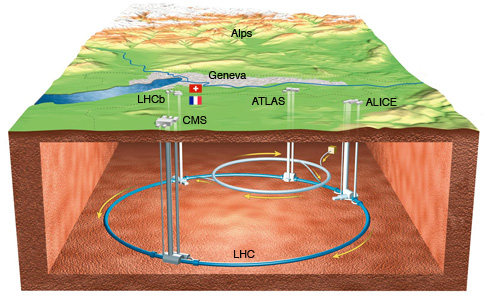
\includegraphics[width=0.7\textwidth]{det/fig/LHC_map}
    \caption{ The LHC tunnel and its four main experiments: ATLAS, ALICE, CMS, and LHCb.}
    \label{fig:det:tunnel}
  \end{center}
\end{figure}

The LHC lies in a 27-km tunnel buried about 170 meters underground (Fig.~\ref{fig:det:tunnel}). Four main experiments are located around the LHC ring. ATLAS and CMS are general-purpose experiments designed to perform precision measurements and discover the Higgs boson and new physics beyond the Standard Model. ALICE studies heavy ion collisions, while LHCb specializes in b-physics and forward measurements.

\subsection{ Beam Structure }
The collider tunnel hosts a super-conducting magnet system that supports two proton beams traveling in opposite directions around the circle. 1232 dipole magnets supply bending power, while 392 quadrupoles keep the beam focused~\cite{Brüning:782076}.

% http://www.lhc-closer.es/1/3/9/0
\begin{figure}[phtb]
  \begin{center}
        \subfigure[Protons colliding in bunches]{%
          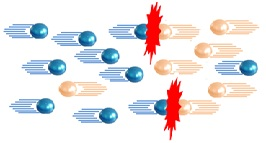
\includegraphics[width=0.44\textwidth]{det/fig/beam}
        } 
        \subfigure[Primary and pile-up interactions]{%
          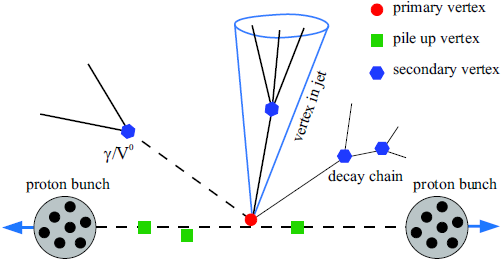
\includegraphics[width=0.44\textwidth]{det/fig/collision}
        }
 \caption{ Diagrams illustrating collision of proton bunches at the LHC.}
 \label{fig:det:bunches}
 \end{center}
\end{figure}

During a ``fill'', which happens approximately once a day, new protons are injected into the beam. They are organized into compact clusters called ``bunches'' that are spread around the circumference of the collider. The exact bunch structure is generally configurable and normally changes throughout the year, but the following are the prevailing conditions during 2011 data-taking~\cite{ATLAS-DAPR-2011-01-002}. The maximum number of bunch pairs in the tunnel at any given time (for clockwise and counterclockwise beams) is 1331. A typical bunch has $1.2 \cdot 10^{11}$ protons, and bunches meet every 50 ns. Despite a huge number of protons in the colliding bunches, each collision produces only about a dozen inelastic interactions. In an overwhelming majority of cases, only one of those interactions, called the ``primary'', produces interesting physics, while the others, called ``pileup'', end up depositing noise in the detector (Fig.~\ref{fig:det:bunches}).

\section{ The ATLAS Detector }

ATLAS (A Toroidal LHC Apparatus) is a complex machine that measures 25 meters in diameter and 46 meters in length, weighing nearly 7000 tonnes~\cite{Aad:2009wy}. It consists of a succession of particle detectors that surround the beam pipe and are centered on the nominal collision point (Fig.~\ref{fig:det:passage}). The innermost layers are instrumented with fine-grained tracking detectors submerged in a two-tesla solenoid field that bends charged particles in the plane transverse to the beam, providing a measurement of their momentum. Next, electromagnetic and hadronic calorimeters measure energy depositions from photons, electrons, and strongly-interacting particles, such as pions, protons and neutrons. Finally, the muon spectrometer, which provides a measurement of muon momentum, contains a variable toroidal magnetic field that bends charged particles in the longitudinal plane.

The detector is largely symmetric around the $\eta=0$ point. By convention, the $\eta<0$ and $\eta>0$ regions are called C-side and A-side, respectively.

\begin{figure}[phtb]
  \begin{center}
    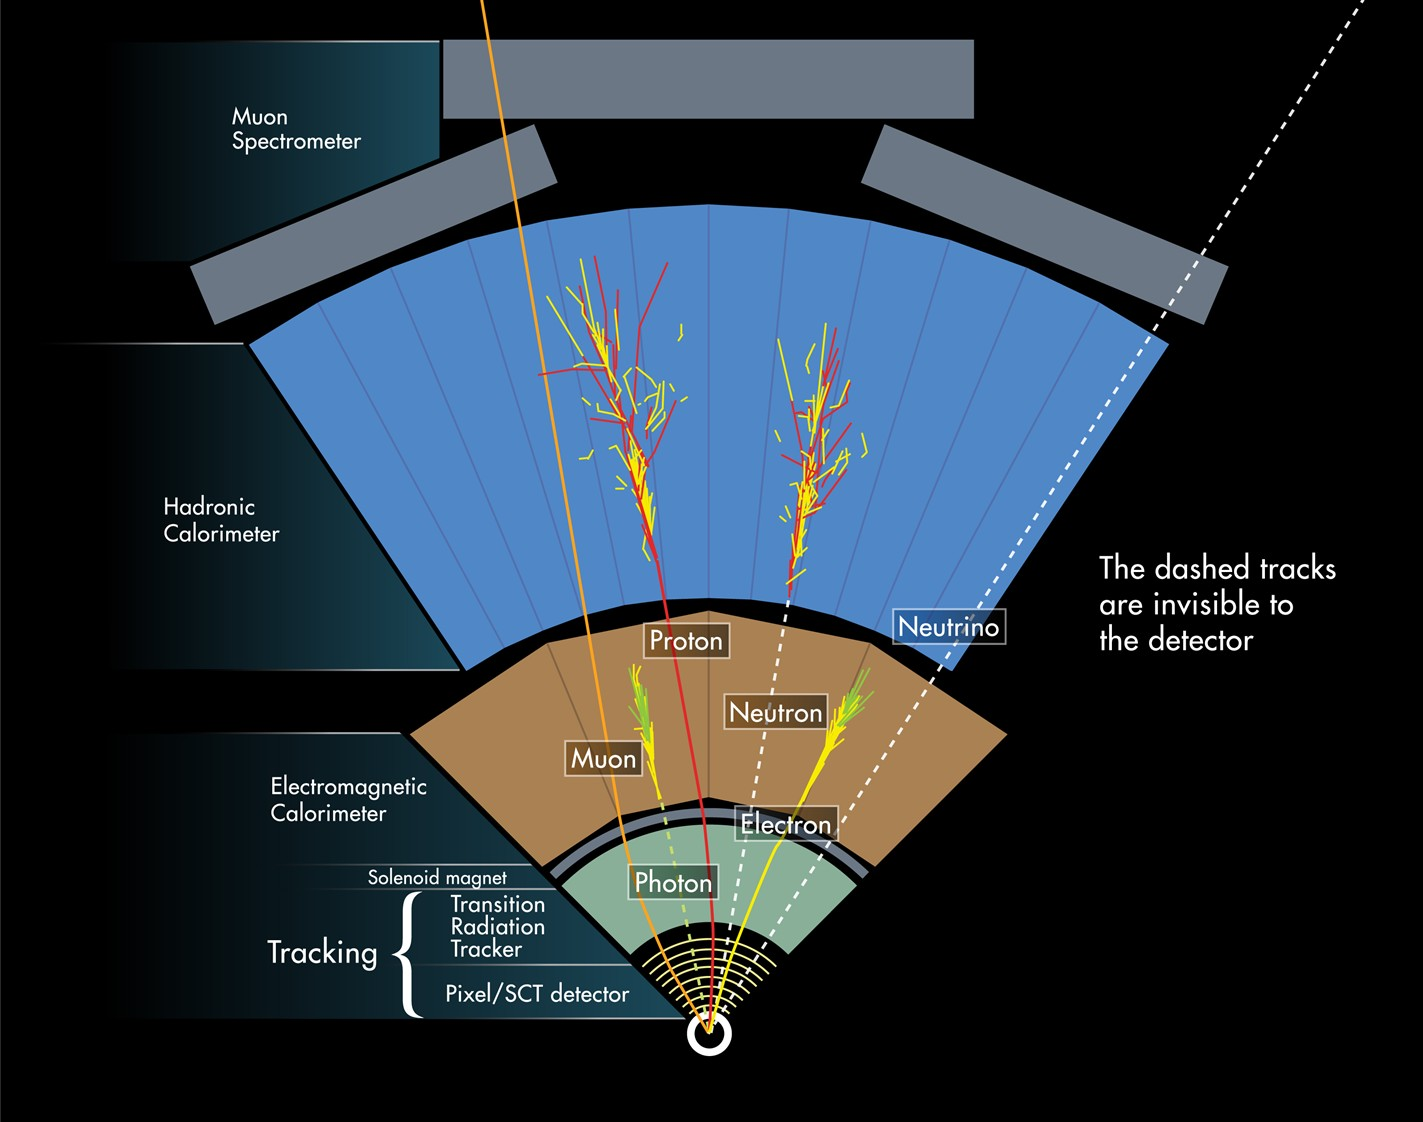
\includegraphics[width=0.80\textwidth]{det/fig/detection}
    \caption{ A diagram showing the ability of different ATLAS components to detect various particles produced in the collisions. }
    \label{fig:det:passage}
  \end{center}
\end{figure}

\subsection{ Inner Detector }
\label{chap:det:id}
The Inner Detector (ID) consists of the Pixel subsystem, Semiconductor Tracker (SCT), and Transition Radiation Tracker (TRT). These detectors play a crucial role in this analysis by measuring $\eta$, $p_{T}$, and other tracking parameters of muons from the \Wmn\ decay.

Fig.~\ref{fig:det:indet_side} shows a side view of the ID subsystems, which altogether span 6.2 meters in length and 2.1 meters in diameter. The region within approximately $|\eta|<1.1$ is called the ``Barrel'', reflecting the fact that the detectors in this region are shaped in barrel-like cylinders concentric around the beam pipe. The more forward region (larger $\eta$) is called the ``Endcap'' and is instrumented with disk-like structures with the sensitive layers positioned radially in the transverse plane.

\begin{figure}[phtb]
  \begin{center}
        \subfigure[Components of the Inner Detector]{%
          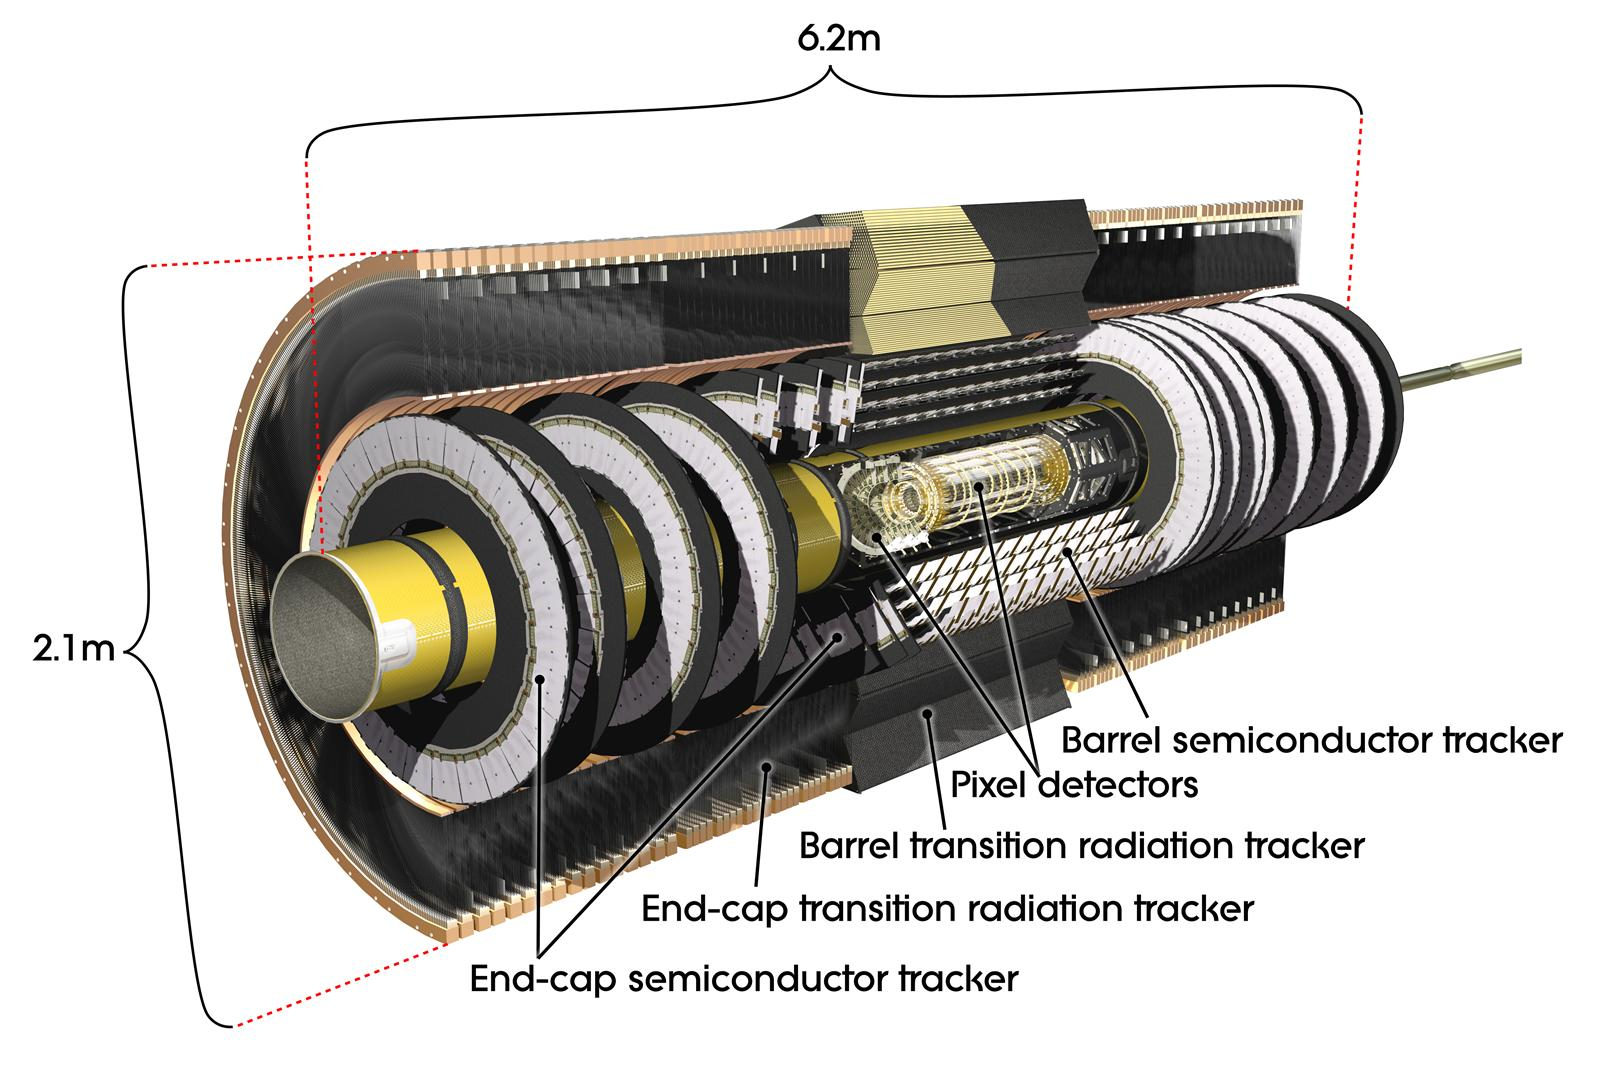
\includegraphics[width=0.8\textwidth]{det/fig/indet_side}
        }  \\
        \subfigure[Side view showing $\eta$ coverage]{%
          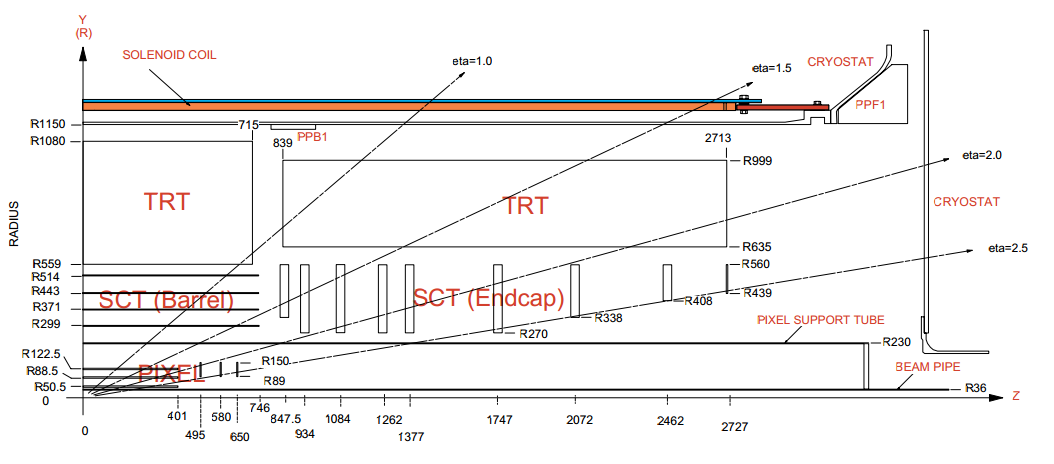
\includegraphics[width=0.8\textwidth]{det/fig/indet_etaview}
        }
 \caption{  Sub-components of the ATLAS Inner Detector and their $\eta$ coverage. }
 \label{fig:det:indet_side}
 \end{center}
\end{figure}

The Pixel detectors provide high-granularity tracking closest to the beam pipe (Fig.~\ref{fig:det:indet_xsec}). Each of the 1744 Pixel modules can be viewed as a two-dimensional sensor grid with $144$ measurement points along the $z$ axis and $328$ along the $R-\phi$ plane. Each sensor is $50$ x $400$ $\mu m^2$ and provides a time-over-threshold measurement of the energy deposited by the particles~\cite{1748-0221-3-07-P07007}. In total, the Pixel detector contains 80.4 million readout channels and is supported by a vast array of readout electronics. Pixel modules are arranged so that a typical track within the fiducial volume ($|\eta|<2.5$) crosses three detection layers.

The SCT detector is located outside of the Pixel system extending up to the radius of 65 centimeters. It consists of 4088 modules instrumented with silicon strips that provide a binary (on-off) readout. SCT modules have two measurement planes with 768 strips each: one plane with strips running parallel to the beam line and measuring hit positions in the $\phi$ direction, and another ``stereo'' plane offset by $40$ $mrad$ and providing information about $\eta$~\cite{1748-0221-3-10-P10006}. The strips are separated by about $80$ $\mu m$. In total, the SCT detector contains 6.3 million readout channels. SCT modules are arranged so that a typical track within the fiducial volume ($|\eta|<2.5$) crosses at least eight detection layers.

% on transition radiation: http://arxiv.org/pdf/hep-ex/0311058v1.pdf
The TRT detector consists of about 350,000 $4$ mm-diameter proportional straw tubes covering the region up to $|\eta|<2.0$. A typical track leaves 30 hits in the detector. The TRT extends to a radius of 1 meter, providing a long lever arm to measure the track parameters. Additionally, the TRT can detect transition radiation (photons emitted when a charged particle moves through an inhomogeneous medium), which is used to distinguish electrons from other minimum-ionizing particles, such as pions~\cite{1748-0221-3-02-P02013}.

\begin{figure}[phtb]
  \begin{center}
    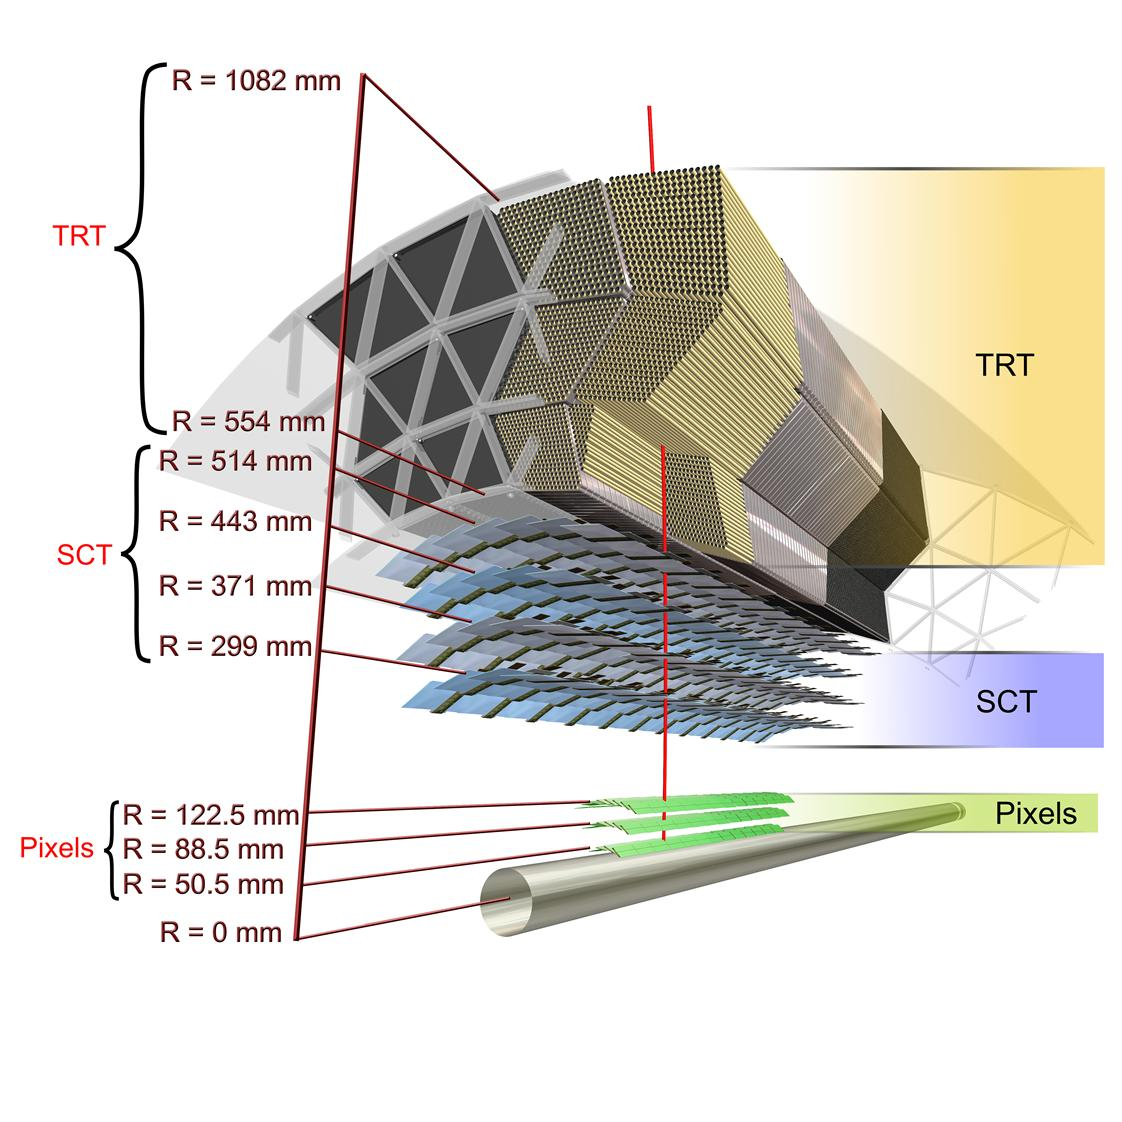
\includegraphics[width=0.70\textwidth]{det/fig/indet_xsec}
    \caption{ Cross-section view of the ATLAS Inner Detector, showing individual Pixel, SCT, and TRT modules. }
    \label{fig:det:indet_xsec}
  \end{center}
\end{figure}

\subsection{ Calorimeters }

Calorimeters are located outside of the Inner Detector solenoid magnet and measure the energy of the particles by absorbing them. The ATLAS calorimetry system consists of two parts: the electromagnetic calorimeter (EM) and the hadronic calorimeter (Fig.~\ref{fig:det:calo}). In the context of this analysis, calorimetry plays a crucial role by measuring the transverse energy imbalance used to identify neutrinos in \Wmn\ decays, which go through the detector unimpeded.

\begin{figure}[phtb]
  \begin{center}
    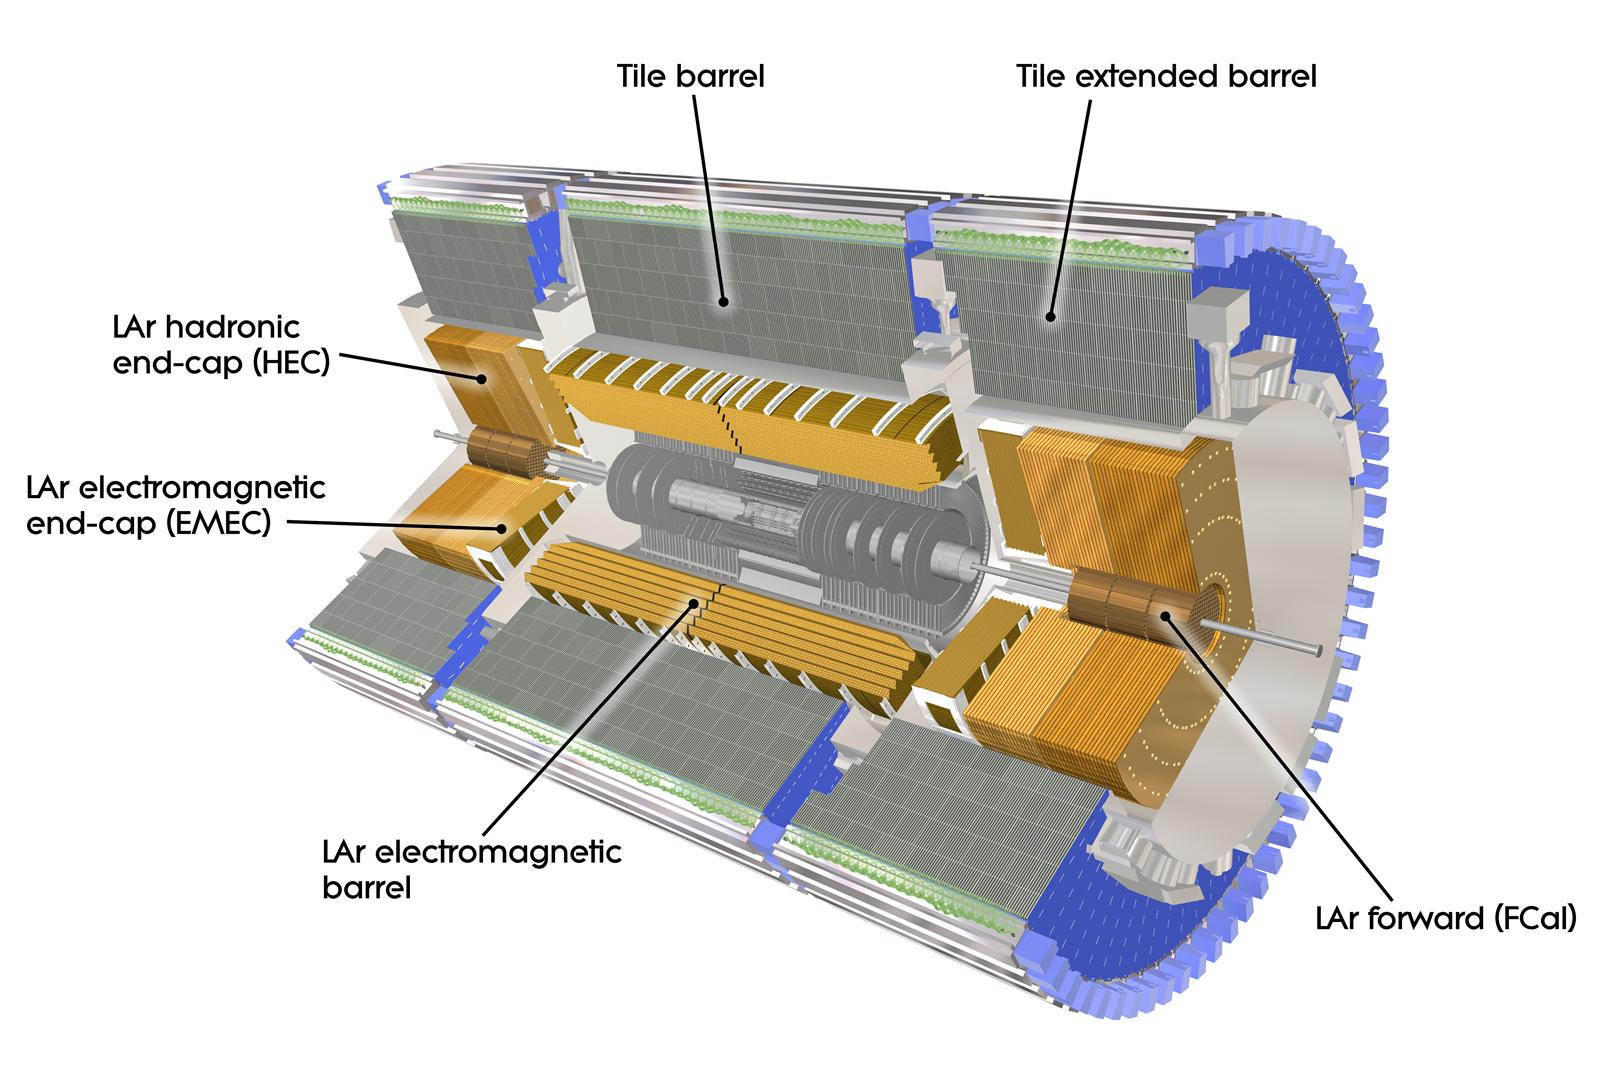
\includegraphics[width=0.80\textwidth]{det/fig/calo}
    \caption{ ATLAS calorimeter system. }
    \label{fig:det:calo}
  \end{center}
\end{figure}

The EM calorimeter, also called a LAr calorimeter, measures the energy of electromagnetically-interacting particles (photons and electrons) up to $|\eta|<3.2$. The active material is liquid argon (LAr), which is interspersed with accordion-shaped absorber plates made of lead or steel (Fig.~\ref{fig:det:accordion}). The total thickness of material is 20-22 radiation lengths, ensuring that the electrons and photos are stopped within the calorimeter~\cite{lar_tdr}. The calorimeter is segmented into 3 sampling layers and has a typical granularity of 0.025 radians in $\Delta\phi$ and $\Delta\eta$.

\begin{figure}[phtb]
  \begin{center}
    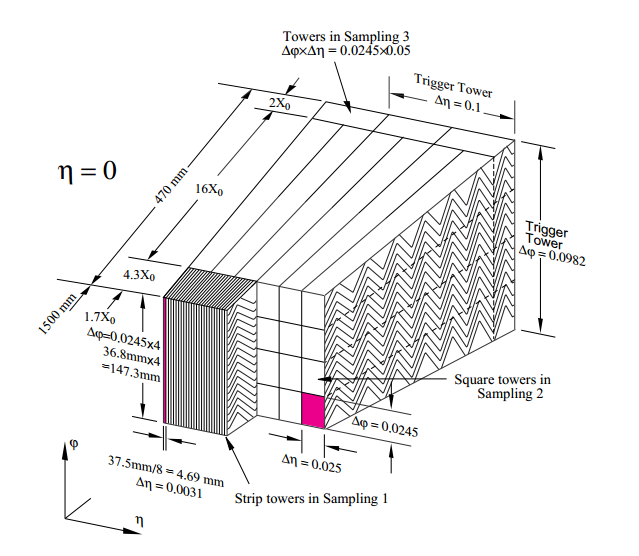
\includegraphics[width=0.70\textwidth]{det/fig/accordion}
    \caption{ Sketch of a section of the barrel EM calorimeter. }
    \label{fig:det:accordion}
  \end{center}
\end{figure}

The hadronic calorimeter measures the energy of strongly-interacting particles, such as pions. Its central portion, called Tile calorimeter, covers up to $|\eta|<1.7$ and uses steel as the absorber and scintillating tiles as the active medium (Fig.~\ref{fig:det:tile}). The tile calorimeter has a typical granularity of 0.1 radians in $\Delta\phi$ and 0.1 in $\Delta\eta$~\cite{tile_tdr} and is instrumental in reconstructing hadronic jets. The total thickness of the material exceeds 10 absorption lengths, which is sufficient to stop most hadrons within the calorimeter. Muons, however, are able to punch through after losing a few GeV in energy. The forward portions of the hadronic calorimeter extend $\eta$ coverage to 4.9 and, like the EM calorimeter, use the LAr technology, but with tungsten-copper absorbers.

\begin{figure}[phtb]
  \begin{center}
    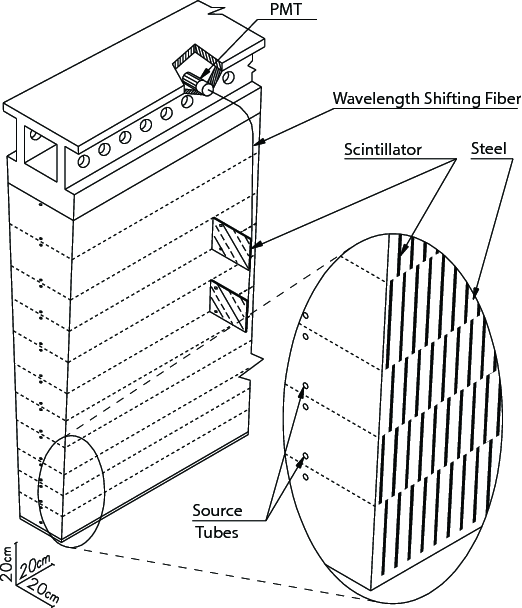
\includegraphics[width=0.50\textwidth]{det/fig/tile}
    \caption{ A wedge of the hadronic Tile calorimeter. }
    \label{fig:det:tile}
  \end{center}
\end{figure}

\subsection{ Muon Spectrometer }
\label{chap:det:ms}
The Inner Detector already measures the momentum of the muons. However, at sufficiently high $p_T$ (above 100 GeV), inner detector tracks look like straight lines, making it difficult to determine the charge (direction of bending) and the precise value of the momentum. The Muon Spectrometer mitigates these deficiencies by providing a much larger lever arm to measure the bending in the toroidal magnetic field. Because the muon spectrometer is placed after the calorimeters, it does not see the electrons or pions and can thus identify the charged particles it sees as muons. To ensure high-quality muon reconstruction, this analysis combines the measurements from the Inner Detector and Muon Spectrometer.

The Muon Spectrometer covers the area up to $|\eta|<2.7$ and consists of about 1300 chambers that go all the way to the outer radius of the ATLAS detector~\cite{muon_tdr}. As seen in Fig.~\ref{fig:det:muons}, a typical muon passes through 3 chambers. Four technologies are used in the muon system. Monitored Drift Tubes (MDT) do tracking in the Barrel while Cathode Strip Chambers (CSC) do the same in the Endcaps. For triggering, Resistive Plate Chambers (RPC) are used in the Barrel and Thin Gap Chambers (TGC) in the endcap. Trigger coverage is generally limited to $|\eta|<2.4$.

\begin{figure}[phtb]
  \begin{center}
        \subfigure[3-dimensional view]{%
          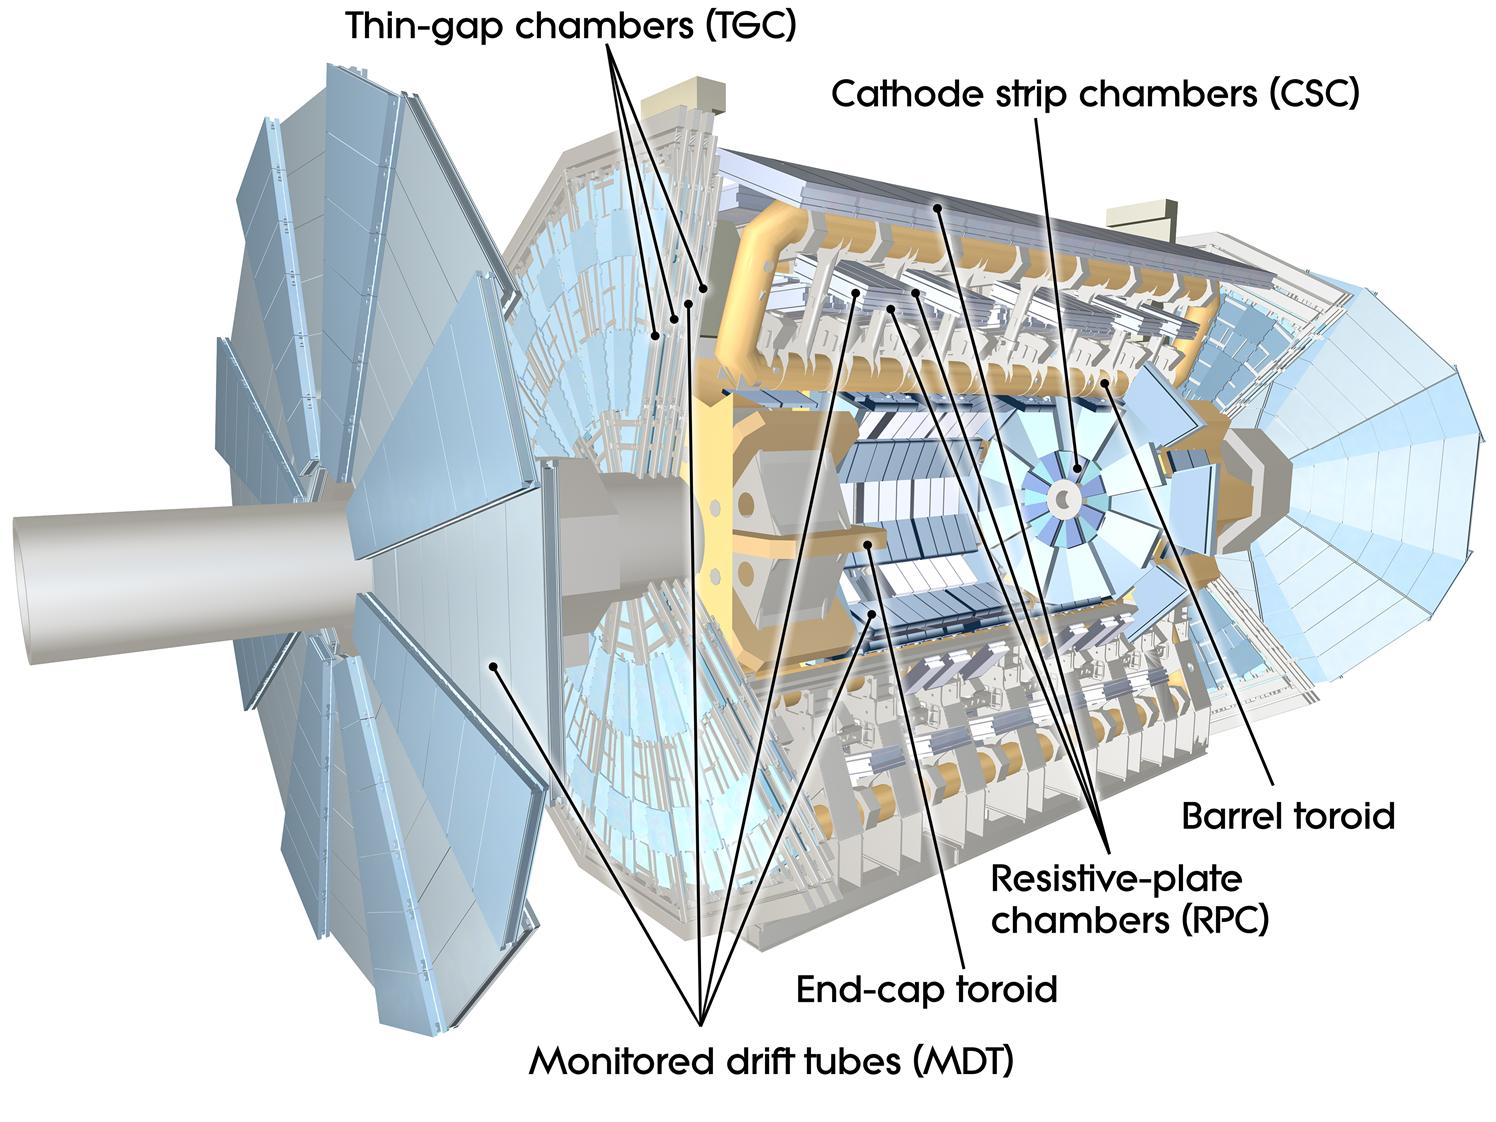
\includegraphics[width=0.7\textwidth]{det/fig/muons}
        }  \\
        \subfigure[Side view]{%
          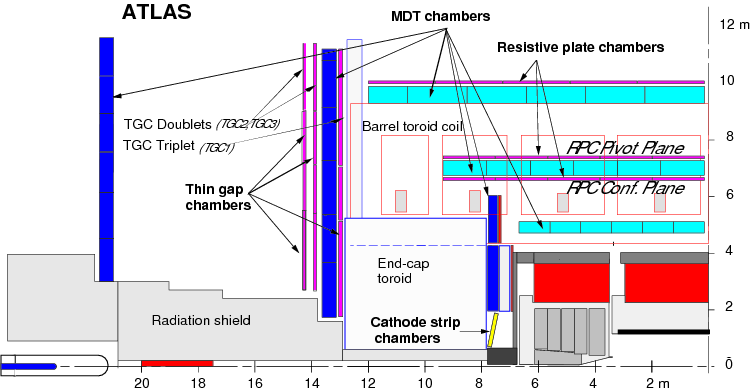
\includegraphics[width=0.8\textwidth]{det/fig/muonside}
        }
 \caption{ A sketch of the main components of the Muon Spectrometer. }
 \label{fig:det:muons}
 \end{center}
\end{figure}

\subsection{ Trigger and Data Acquisition }
\label{sec:det:trigger}
In 2011, the LHC collided proton bunches every 50 ns. Only a tiny fraction of these collisions can be stored for subsequent analysis, and immense real-time data reduction is needed that can select interesting physics while discarding un-eventful collisions. The ATLAS experiment employs a sophisticated three-level trigger system to achieve these goals~\cite{Jenni:616089}. Level-1 selection is performed in dedicated hardware that uses coarse-granularity information from calorimeters and muon spectrometers to apply cuts to a variety of objects, such as jets, muons, electromagnetic clusters, and missing energy. Level-2 and Event Filter, collectively known as High Level Triggers (HLT), are effectively large computer farms designed to refine the selection. Level-2 does limited reconstruction (including tracking) inside Regions of Interest (ROI) identified by the Level-1 trigger. Event Filter performs full-event reconstruction with near-offline quality. The events passing Event Filter are saved on disk.

As Fig.~\ref{fig:det:trigger} shows, the trigger system reduces event rate from 40 MHz down to 200 Hz - a 5-order of magnitude reduction.

\begin{figure}[phtb]
  \begin{center}
    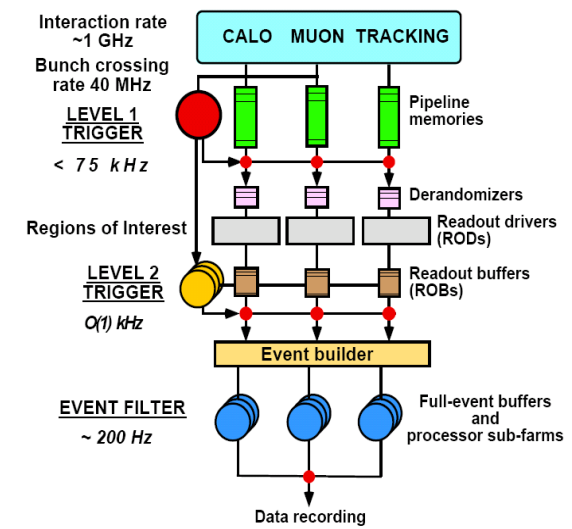
\includegraphics[width=0.60\textwidth]{det/fig/trigger}
    \caption{ The ATLAS trigger system. }
    \label{fig:det:trigger}
  \end{center}
\end{figure}


\subsection{ Computing }
% http://cds.cern.ch/record/840543/files/lhcc-2005-024.pdf

All data collected by ATLAS is initially stored at a central facility at CERN called Tier-0 and subsequently distributed to national Tier-1 centers. The US Tier-1 facility is located at the Brookhaven National Laboratory (BNL). Portions of the data are further replicated to regional Tier-2 facilities, one of which - the Midwest Tier-2 - is located at the University of Chicago. Altogether, the LHC Computing Grid consists of about 170 computing centers around the world, which provide over 200,000 CPUs and hundreds of petabytes of storage for data and Monte-Carlo processing~\cite{Eck:840543,citeulike:8657322}.

All data and Monte-Carlo datasets used in this analysis amount to about 500 terabytes in size. A data reduction algorithm running on the cloud converts these datasets to a more manageable set of ntuples requiring 5 terabytes of storage. These ntuples are stored at the Midwest Tier-2 facility and analyzed with about 1000 CPUs available at the university.



%4
\chapter{Theoretical Overview}
\label{chap:th}
% theoretical overview

\def\sighat{\hat{\sigma}}

\section{Standard Model}
% http://pdg.lbl.gov/2013/reviews/rpp2012-rev-standard-model.pdf

All known interactions can be described by four fundamental forces. Listed in the increasing order of strength, they are: gravity, the weak nuclear force, electromagnetism, and the strong nuclear force. While Albert Einstein's general theory of relativity provides an excellent classical description of gravitational interactions on the macroscopic scales~\cite{GRcite}, a consistent quantum theory of gravity continues to elude theoretical physicists. However, in the domain of physics probed in this thesis, gravity is completely negligible, being 32 orders of magnitude smaller than the weak nuclear force.\footnote{In natural units, the ratio of forces corresponds to the ratio-squared of W boson mass (80 GeV) to Planck mass (1e18 GeV). This large discrepancy is better known as the ``hierarchy problem''.}

The remaining three forces can be interpreted in the quantum-theoretical framework of the Standard Model of particle physics (Fig.~\ref{fig:theory:SM}). A non-abelian gauge theory with the symmetry group $SU(3)$x$SU(2)$x$U(1)$, the Standard Model postulates that all matter is made of fermions (quarks and leptons), which are arranged into three generations separated by different flavor quantum numbers and masses. Interactions between fermions are mediated by the exchange of gauge bosons: $SU(3)$ generates gluons that carry the strong nuclear force, $SU(2)$ generates W bosons responsible for the weak charged currents, while the linear combination of neutral bosons from $SU(2)$ and $U(1)$ produces Z bosons, which mediate weak neutral currents, and photons, which mediate the electromagnetic force. Finally, a complex scalar field generates masses of elementary particles through the Higgs mechanism~\cite{PhysRevLett.13.508}.

This thesis focuses on the measurement of the production cross-section of \Wboson\ gauge bosons at the LHC. The mechanism of \Wboson\ production is explored in the next section.

\begin{figure}[phtb]
  \begin{center}
    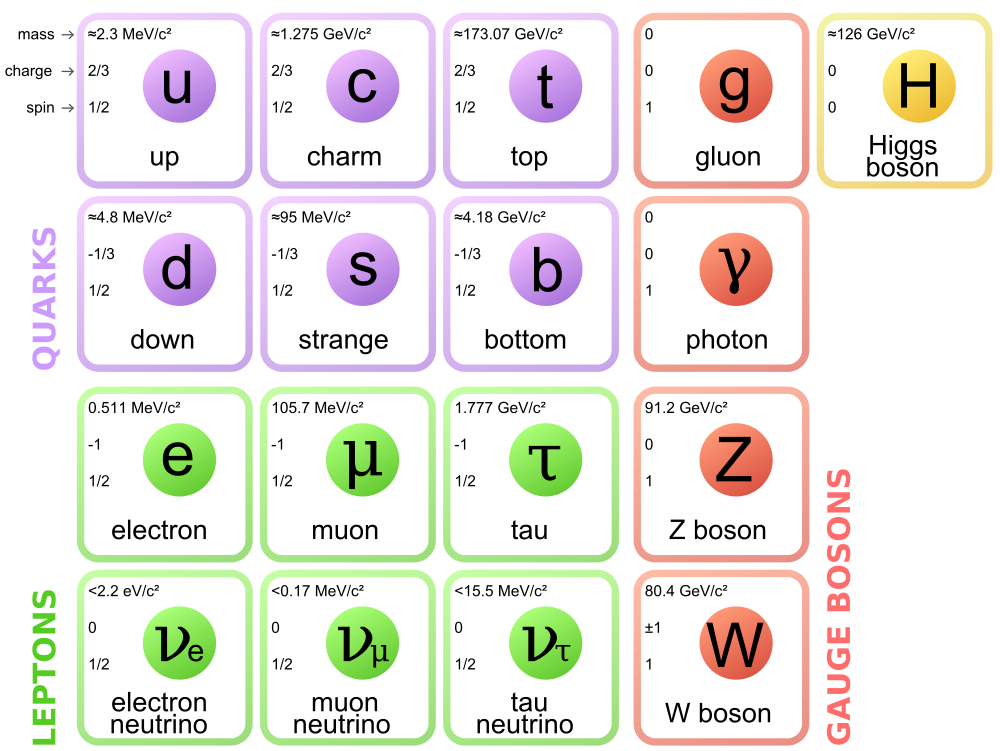
\includegraphics[width=0.7\textwidth]{theory/fig/SM}
    \caption{ The Standard Model of elementary particles.}
    \label{fig:theory:SM}
 \end{center}
\end{figure}

\section{ Hadron Scattering }
\label{chap:qcd_theory}

% Electroweak W gauge bosons are produced through proton-proton scattering at the LHC. 

In the first half of the 20th century, protons were considered to be point particles that, along with neutrons, combined to form the nuclei of all known atoms. Deep inelastic scattering experiments, which involve bombardment of protons by electrons, revealed non-trivial compositeness of the proton and led to the development of the parton model~\cite{PhysRevLett.23.1415}.

Under the parton model, protons consist of three valence quarks: two of up-type and one of down-type. These quarks spontaneously produce gluons, which in turn can split into additional quark-antiquark pairs, known as ``sea quarks''. Collectively, this swarm of constituents inside the proton are called partons. The fraction of the total proton momentum carried by each constituent is conventionally labeled ``x'', which varies from 0 to 1. Parton distribution functions (PDFs) are probability distributions of $x$ for different kinds of partons (see Sec.~\ref{chap:pdf_theory}).

According to the factorization theorem postulated by Drell and Yan~\cite{PhysRevLett.25.316}, a hard scattering collision between protons $A$ and $B$ can be viewed as an interaction between two free partons $a$ and $b$ with respective momentum fractions $x_a$ and $x_b$, weighted by the probability of carrying these momentum fractions (PDFs). The parton-parton interaction can be calculated in the context of perturbative quantum chromodynamics (QCD), amounting to a calculation of the relevant Feynman diagrams to a given order. The PDFs, however, are not calculable from the first principles and have to be determined experimentally. The key statement of the factorization theorem, illustrated in Fig.~\ref{fig:theory:hardscatter}, is that the PDFs are independent of the parton-parton process.

\begin{figure}[phtb]
  \begin{center}
    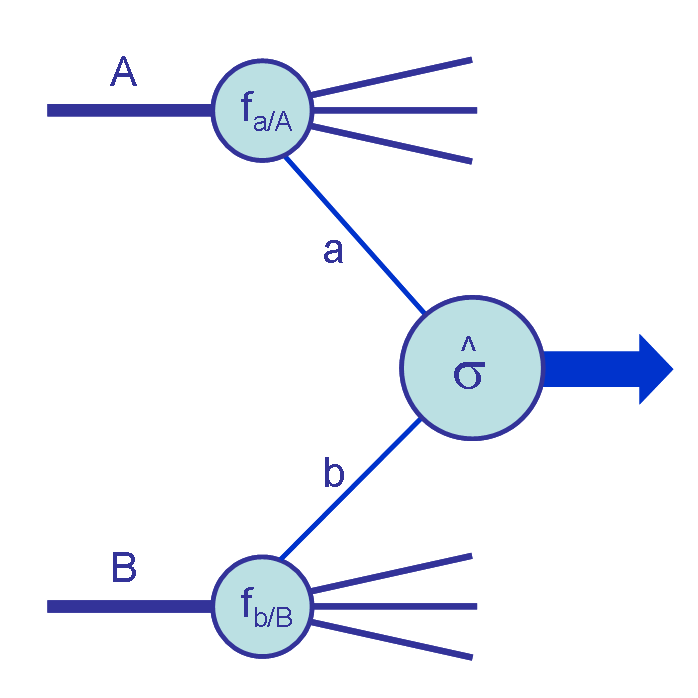
\includegraphics[width=0.4\textwidth]{theory/fig/Hardscattering}
    \caption{ Illustration of the factorization theorem in a hard-scattering process. $\sighat$ is the hard scattering cross-section, while small f's represent PDFs for each incoming proton. }
    \label{fig:theory:hardscatter}
 \end{center}
\end{figure}

Mathematically, the factorization theorem allows the cross-section of $AB\to W$ (where A,B are incoming protons) to be expressed by the following formula:
\begin{equation}
\begin{split}
\sigma_{AB\to W} = \sum\limits_{partons} \int dx_a dx_b\; f_{a/A}(x_a,\mu_{F}^2) f_{b/B}(x_b,\mu_{F}^2) \cdot \\
\left[ \sighat_{LO}(x_{a}x_{b}s) + \alpha_{s}(\mu_{R}^2)\sighat_{NLO}(x_{a}x_{b}s) + \left(\alpha_{s}(\mu_{R}^2)\right)^{2}\sighat{NNLO}(x_{a}x_{b}s) + \ldots \right]
\end{split}
\label{sigll}
\end{equation}
The meaning of all variables is explained below.

The partonic cross-section $\sighat$ is expanded in powers of the strong interaction coupling constant $\alpha_{s}$, where higher-order perturbation terms correspond to Feynman diagrams with additional emissions. The cross-section at each order depends on the energy scale $Q^2 \equiv x_{a}x_{b}s$, where $\sqrt s$ is the center-of-mass energy of proton collisions. $\alpha_{s}$ depends on a non-physical parameter $\mu_{R}$ - the renormalization scale of the QCD running coupling. Intuitively, renormalization avoids ultraviolet infinities in higher-loop diagrams by re-defining the coupling constant when probing the interaction at different energy scales. The PDFs $f_{a/A}(x_a,\mu_{F}^2)$\footnote{$f_{a/A}$ refers to a parton $a$ from the incoming hadron $A$} and $f_{b/B}(x_b,\mu_{F}^2)$ depend on another non-physical parameter $\mu_{F}$, known as the factorization scale. This is the energy scale that separates perturbative and non-perturbative pieces of the calculation, with the latter being absorbed into the definition of the PDF. These non-perturbative elements correspond to soft collinear gluon emissions, which produce infrared singularities in the perturbation theory.

In principle, the numerical cross-section is independent of the renormalization and factorization scales, with all non-physical dependencies canceling out if the series expansion is carried to all orders of $\alpha_{s}$. However, because practical considerations require that the calculation is stopped early (usually at NLO or NNLO), some dependence of the cross-section on these non-physical parameters is retained. The conventional prescription is to choose $\mu_{R}$ and $\mu_{F}$ to be of the same order as the typical momentum transfer in the hard scattering process. More specifically, $\mu_{R}$ and $\mu_{F}$ are both set to the mass of the produced \Wboson\ boson, but are allowed to vary by a factor of 2 of their central values, resulting in additional theoretical uncertainty on the cross-section.

\subsection{W production}

The leading-order diagram for \Wboson\ production is shown in Fig.~\ref{fig:theory:feynlo}.

\begin{figure}[phtb]
  \begin{center}
    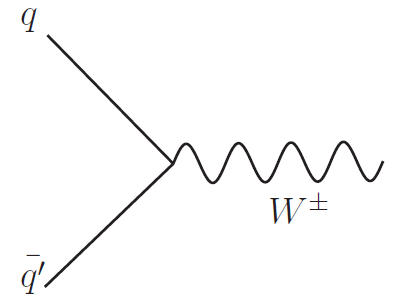
\includegraphics[width=0.3\textwidth]{theory/fig/feynlo}
    \caption{ Leading-order diagram of \Wboson\ production through quark-antiquark annihilation.}
    \label{fig:theory:feynlo}
 \end{center}
\end{figure}

The cross-section $\sighat$ of this diagram can be calculated with standard quantum field theory techniques and yields~\cite{PDG}:
$$ \sighat(q\bar{q'} \rightarrow W) = 2\pi|V_{qq'}|^2 \frac{G_F}{\sqrt{2}} M_{W}^{2} \cdot \delta\left(Q^2 - M_{W}^{2}\right)$$
where $G_F$ is the Fermi coupling constant, $|V_{qq'}|$ is the relevant element from the Cabibbo-Kobayashi-Maskawa (CKM) quark mixing matrix~\cite{Kobayashi01021973}, $M_W$ is the mass of the W boson, and $\delta$ is the Dirac delta function. Beyond leading order, the relationship becomes more complex, and the restriction on $Q^2=M_{W}^{2}$ is relaxed.

Fig.~\ref{fig:theory:Wprod} shows that the dominant production channel for $W^+$ is through $u\bar{d}$, where the up quark is a valence quark while the anti-down comes from the sea (and similarly for $W^-$ with $\bar{u}d$). At 7 TeV, about 10\% of \Wboson\ bosons are produced through strange-charm annihilation, followed by a negligible contribution from CKM-suppressed cross-family processes.

\begin{figure}[phtb]
  \begin{center}
    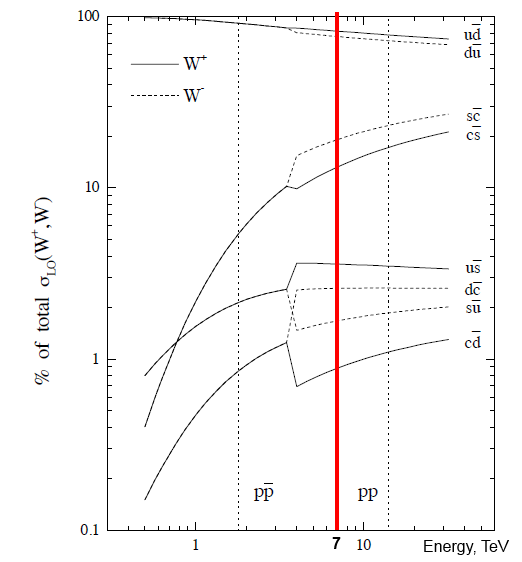
\includegraphics[width=0.55\textwidth]{theory/fig/Wprod}
    \caption{ Contributions of several quark-antiquark processes to \Wboson\ production cross-section. The red line marks the collision energy relevant to this analysis (7 TeV). }
    \label{fig:theory:Wprod}
 \end{center}
\end{figure}

\subsection{Parton Distribution Functions}
\label{chap:pdf_theory}

Parton distribution functions quantify the probability distributions of the momentum fraction $x$ for partons within a hadron. They are not calculable from first principles in perturbation theory and have to be determined experimentally through a global fit to various experimental data~\cite{pdfmaster}. Because experiments may operate at different energy transfer points, the PDFs are extrapolated to a common energy scale $Q^2$ in fits to experimental data, which is accomplished through the so-called DGLAP evolution equations~\cite{Dokshitzer:1977sg,Gribov:1972ri,Altarelli:1977zs}. Similar to scattering amplitude calculations, PDFs can be defined at different orders of perturbation theory.

By way of introduction, suppose $u(x)$ and $d(x)$ are PDFs for up and down quarks, while $\bar{u}(x)$ and $\bar{d}(x)$ are PDFs of the corresponding anti-quarks. In a proton, valence quarks are identified as $u_v=u-{\bar u}$ and $d_v=d-{\bar d}$, which implies the following constraints on the proton PDFs~\cite{0034-4885-76-4-046201}:
\begin{eqnarray}
\int_0^1 \left[u(x)-\bar{u}(x) \right] \, {\rm d}x = 2   \hspace{2cm}  
\int_0^1 \left[d(x)-\bar{d}(x) \right] \, {\rm d}x = 1 \,\,\,   \label{eq:countingrule} \\
{\rm{and}} \hspace{1cm} \int_0^1 \left[q(x)-\bar{q}(x) \right] \, {\rm d}x = 0 \hspace{1cm} {\rm{for }} \quad q=s,c,b,t
\label{eq:countingrule2}
\end{eqnarray}

Fig.~\ref{fig:example_pdfs} shows an example of proton PDFs from the CT10 collaboration~\cite{Lai:2010vv} at two different $Q^2$ scales. From the PDF curves, one sees that (1) valence quarks tend to carry a much higher fraction of proton momentum, and (2) gluon and sea quark distributions increase dramatically at higher energy scales.

\begin{figure}[htb]
\begin{center}
\begin{tabular}{cc}
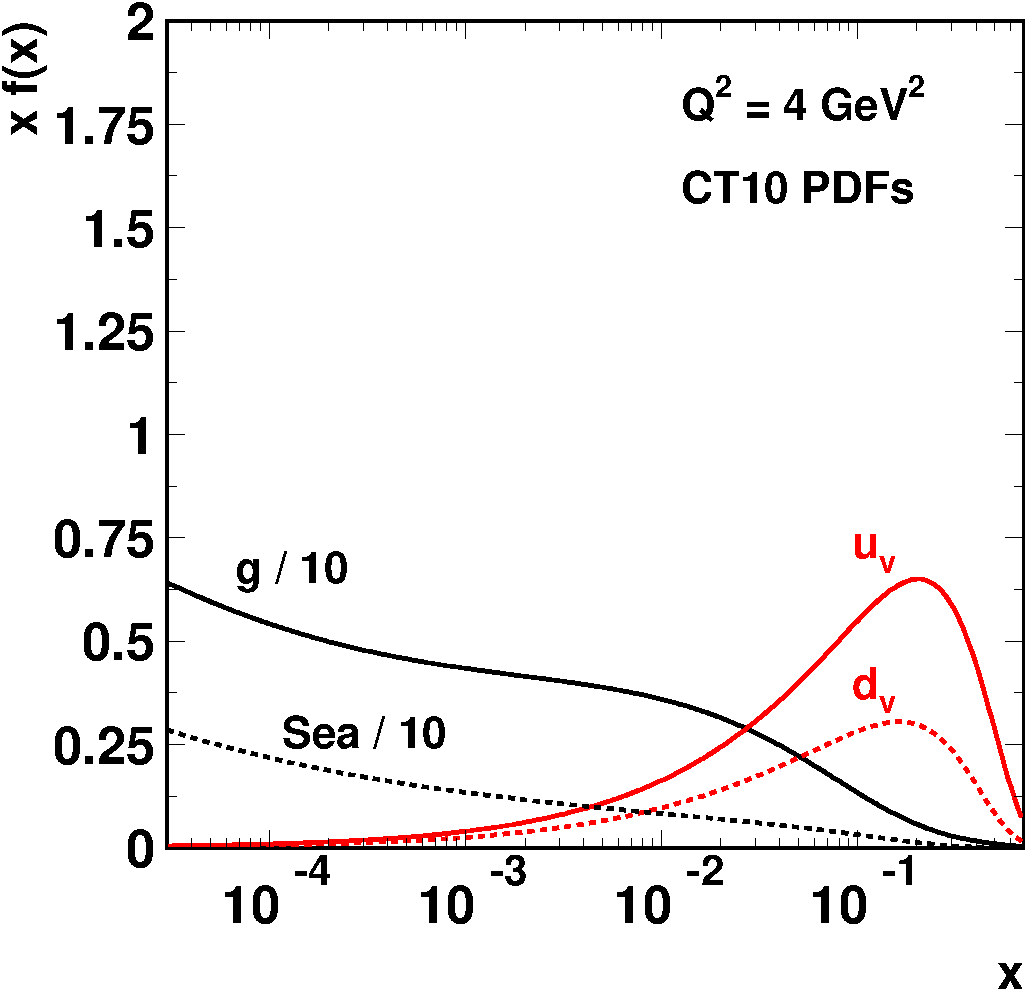
\includegraphics[width=0.45\columnwidth]{theory/fig/examplepdfs_q2} &
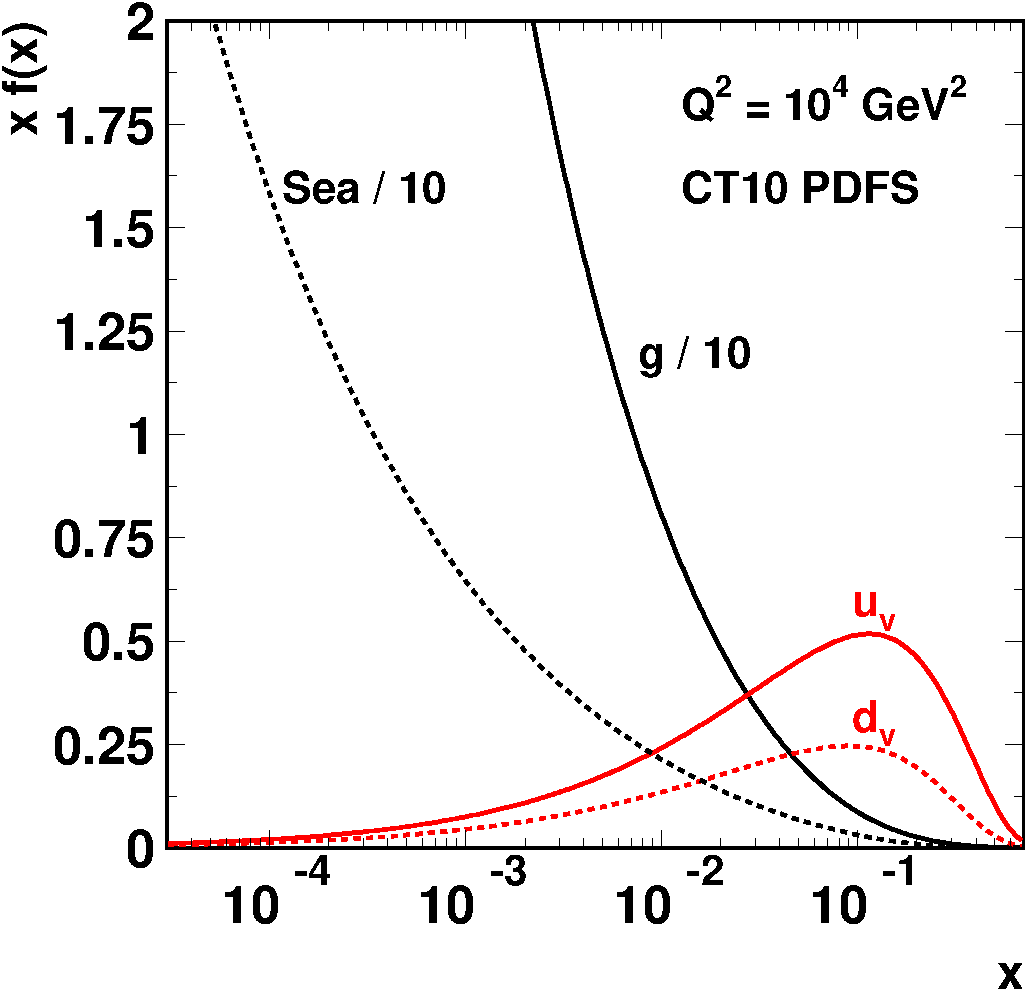
\includegraphics[width=0.45\columnwidth]{theory/fig/examplepdfs_q100}
\end{tabular}
\end{center}
\caption{ Example PDFs at $Q^2 = 4$~GeV$^2$ and $Q^2 = 10^4$~GeV$^2$ (CT10 collaboration). }
\label{fig:example_pdfs}
\end{figure}

PDFs always come with an uncertainty band, which was not shown in Fig.~\ref{fig:example_pdfs}. This uncertainty is driven by experimental uncertainties in the input data and may be amplified by DGLAP evolution to a common energy scale $Q^2$. PDF uncertainties often play an important role in searches for new physics and precision measurements at collider experiments, so a lot of work has gone into developing robust PDF families~\cite{Alekhin:2012ig,Aaron:2009aa,Radescu:2011cn,Martin:2009iq,Ball:2012cx}. Global PDF fits can greatly benefit from new data inputs, particularly in sparsely studied regions of phase space. For example, Fig.~\ref{fig:theory:WZ_str_pdf_ratio} shows the effect of 2010 and 2011 W/Z inclusive cross-section measurements (this thesis is part of the latter) on the strange quark PDF uncertainty bands.

\begin{figure}[phtb]
  \begin{center}
    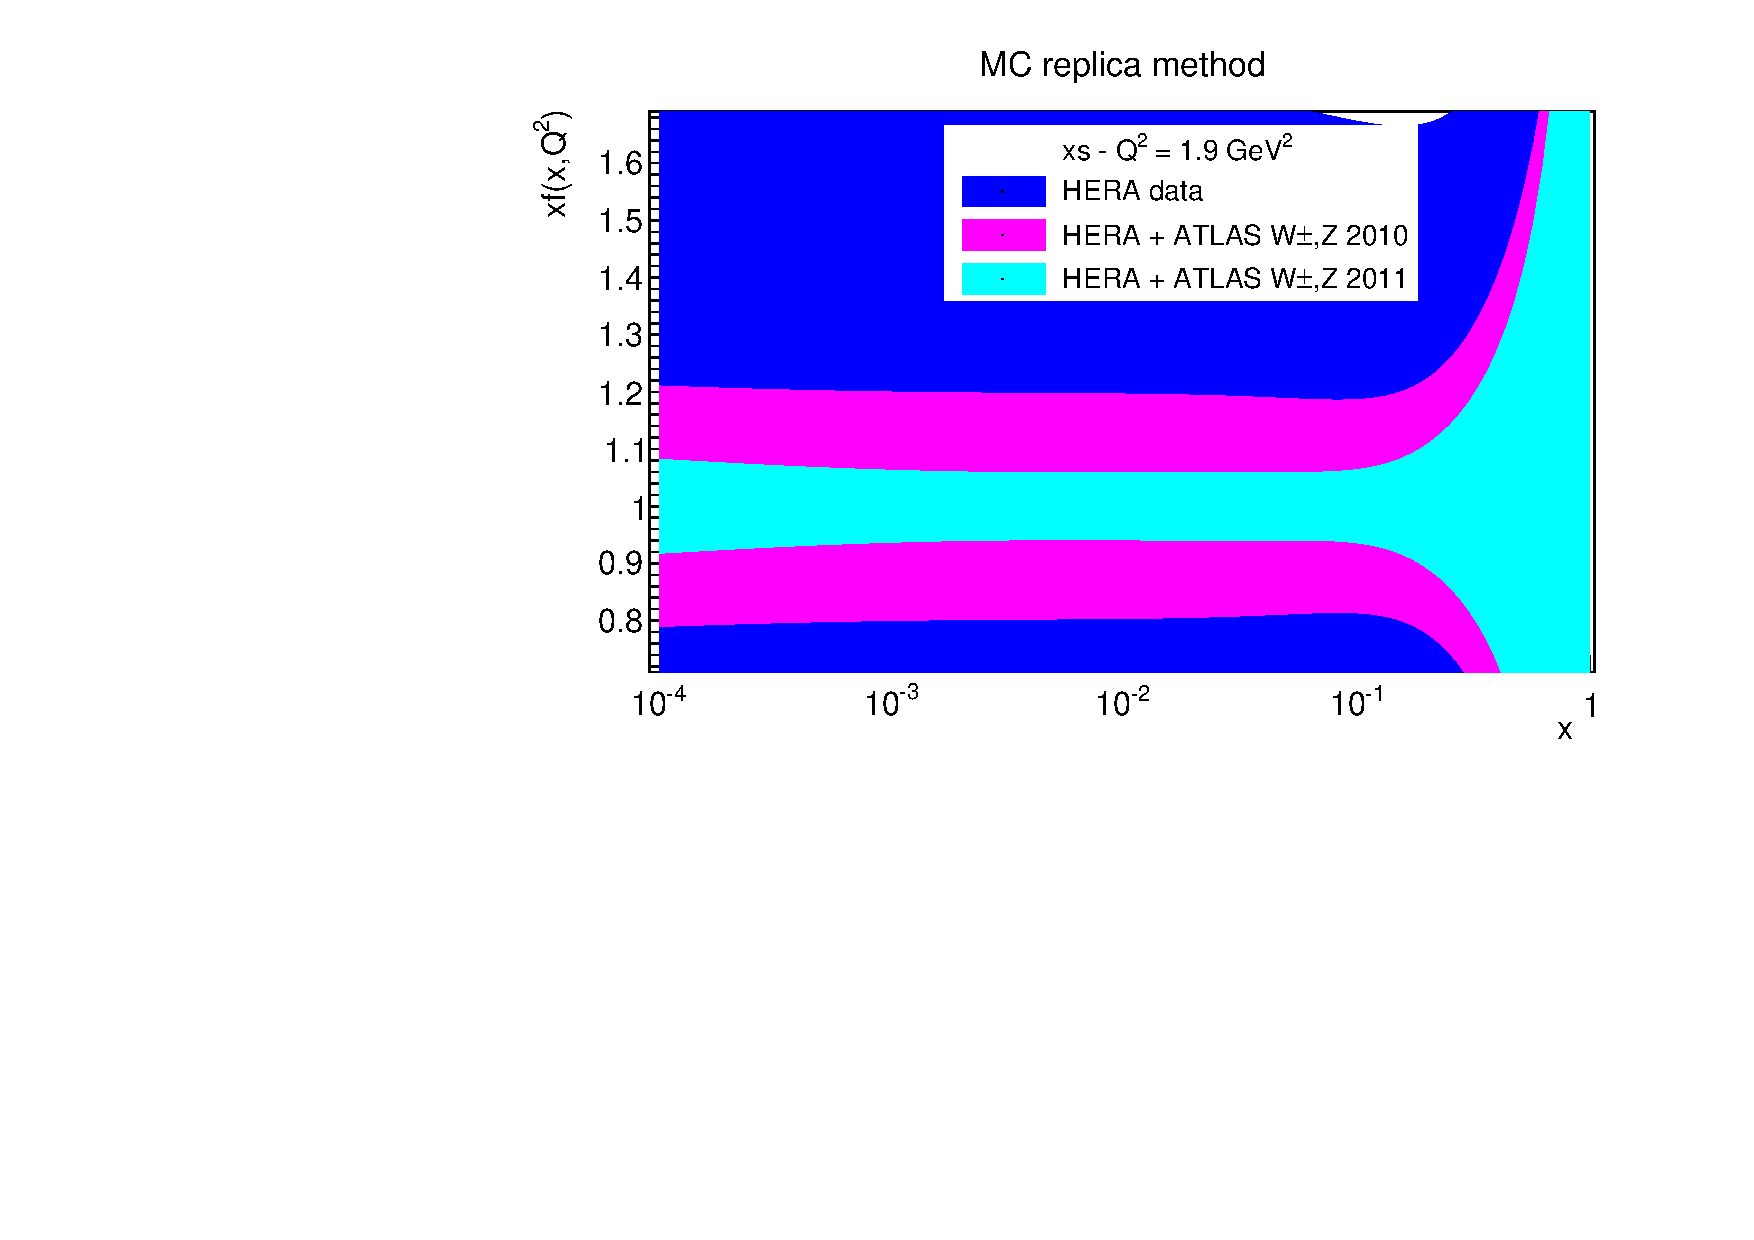
\includegraphics[width=0.7\textwidth]{theory/fig/WZ_str_pdf_ratio}
    \caption{ Strange quark PDFs using deep inelastic scattering data (HERA) alone, with the 2010 W/Z measurement, and with the 2011 W/Z measurement. Shaded regions represent 68\% confidence bands.}
    \label{fig:theory:WZ_str_pdf_ratio}
 \end{center}
\end{figure}

PDF coverage of different experiments is shown in Fig.~\ref{fig:theory:atlas_xq}. The high-$x$, low-$Q^2$ region is dominated by the fixed target experiments. A large region of phase space is covered by deep inelastic scattering data (for example, the solid orange HERA H1 curve). Higher $Q^2$ regions are best constrained by the hadron collider experiments. The measurement performed in this thesis provides the strongest sensitivity at $Q^2=M_{W}^2=80.4^2 GeV^2$ and $0.001<x<0.1$.

\begin{figure}[phtb]
  \begin{center}
    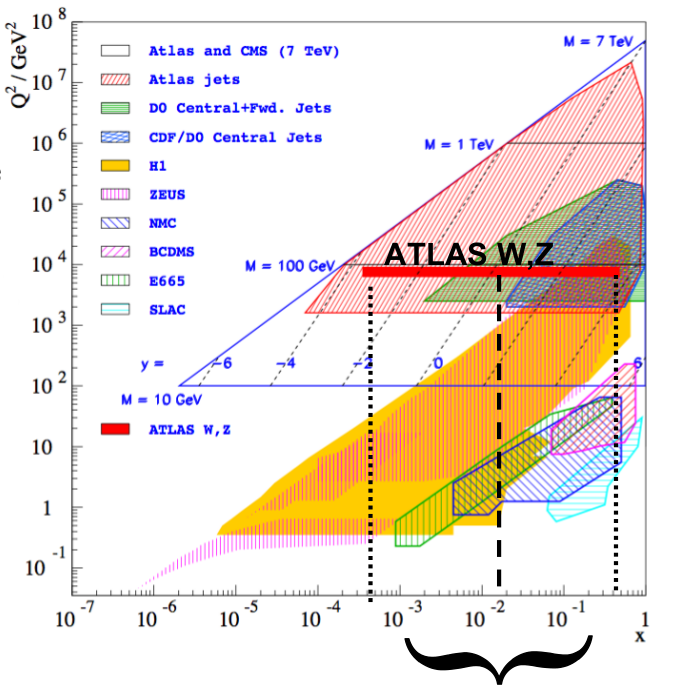
\includegraphics[width=0.5\textwidth]{theory/fig/atlas_xq}
    \caption{ Sensitivity region of various experimental inputs in constraining PDFs.}
    \label{fig:theory:atlas_xq}
 \end{center}
\end{figure}

\subsection{ PDFs and W rapidity }
\label{sec:theory:pdfrap}
Proton structure can be probed in a \Wboson\ cross-section measurement by looking at the boson rapidity $y$, defined as the boost along the beam axis from the lab frame to the frame where the boson moves only perpendicularly to the beam. Note that the pseudorapidity $\eta$ is equal to rapidity $y$ in the limit where $E \gg m$, where $E$ is energy and $m$ is mass.

Boson rapidity is related to parton momentum fractions $x_a$ and $x_b$ through the following relationship:
\begin{equation}
y_W \equiv \frac{1}{2} \cdot ln \left( \frac{E + p_z}{E - p_z} \right) = \frac{1}{2} \cdot ln \left( \frac{x_a}{x_b}\right)
\label{theory:rapidity}
\end{equation}

Setting $Q^2 = m_W^2$ and using the fact that $Q^2 = x_{a}x_{b}s$, we arrive at a direct relationship between the boson rapidity and PDF momentum fractions of the quark-antiquark pair that annihilate to produce the \Wboson\ boson:
$$ x_a = \frac{m_W}{\sqrt s} e^{y_W} $$
$$ x_b = \frac{m_W}{\sqrt s} e^{-y_W} $$

Intuitively, the relationship makes sense: if $x_a$ is substantially higher than $x_b$, the parton coming from proton A will carry a greater momentum and the \Wboson\ boson will be produced moving along the beam axis, which is an intuitive proxy for the boson rapidity.

\section{W Decay and Muon Pseudorapidity}

Fig.~\ref{fig:theory:decay} shows the decay channel studied in this thesis: \Wmn.

\begin{figure}[phtb]
  \begin{center}
    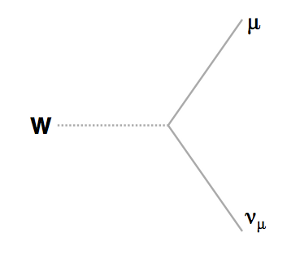
\includegraphics[width=0.25\textwidth]{theory/fig/decay}
    \caption{ Decay of the \Wboson\ boson into a muon and a neutrino.}
    \label{fig:theory:decay}
 \end{center}
\end{figure}

Reconstructing boson rapidity requires information about all three components of the muon and neutrino momenta. However, the $p_z$ component of the neutrino is inaccessible experimentally: only the transverse component $p_T$ is measured through the missing transverse energy. As a result, measurement of the \Wboson\ rapidity requires imposition of a \Wboson\ mass constraint, which produces a quadratic equation for the missing longitudinal component of neutrino momentum. The ambiguity in selecting the correct solution of that quadratic equation renders boson rapidity undesirable in studying the proton structure.

\begin{figure}[phtb]
  \begin{center}
    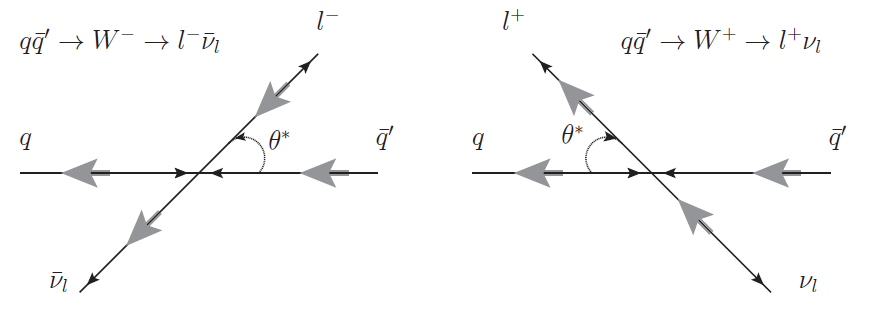
\includegraphics[width=0.7\textwidth]{theory/fig/VA}
    \caption{ Decay diagrams in the rest frame of the \Wboson. Black arrows show the direction of motion; gray arrows indicate the spin. The \Wboson\ spin always points in the direction of the incoming anti-quark.}
    \label{fig:theory:va}
 \end{center}
\end{figure}

A good alternative is to measure the pseudorapidity $\eta$ of the muon, which does not require any knowledge about neutrino $p_z$. The vector minus axial-vector (V-A) nature of the \Wboson\ decay preserves the correlation between boson rapidity $y_W$ and muon pseudorapidity $\eta_\mu$~\cite{MartinezOutschoorn:2011hta}. Fig.~\ref{fig:theory:va} shows preferred decay orientations in terms of $\theta^*$, the angle between the muon in the \Wboson\ rest frame and the direction of the \Wboson, which is distributed according to:
$$ \frac{dN}{d \cos(\theta^*)} = \left(1 \pm \cos(\theta^*) \right)^{2}$$
The sign depends on the product of the W and muon helicities.

As a result, it is possible to deduce information about parton momentum fractions from the pseudorapidity distribution by de-convolving the known V-A correlation between the boson rapidity and the muon pseudorapidity.

\section{Parton Shower and Hadronization}

In addition to the physics of hard collisions outlined above, several additional effects must be considered to fully understand an event at the hadron collider (Fig.~\ref{fig:theory:ps}).

Particles leaving the hard scattering vertex are able to radiate additional particles, which must be taken into account by Monte-Carlo programs. This process is called parton showering (PS), and several variations exist differing in the exact treatment of additional emissions (for example, angular-ordered or virtuality-ordered).

Hadronization is the process by which particles carrying color, which cannot exist in free form, recombine into colorless duplets or triplets. As with parton showering, several implementations are available in Monte-Carlo programs, such as the string or cluster model.

\begin{figure}[phtb]
  \begin{center}
    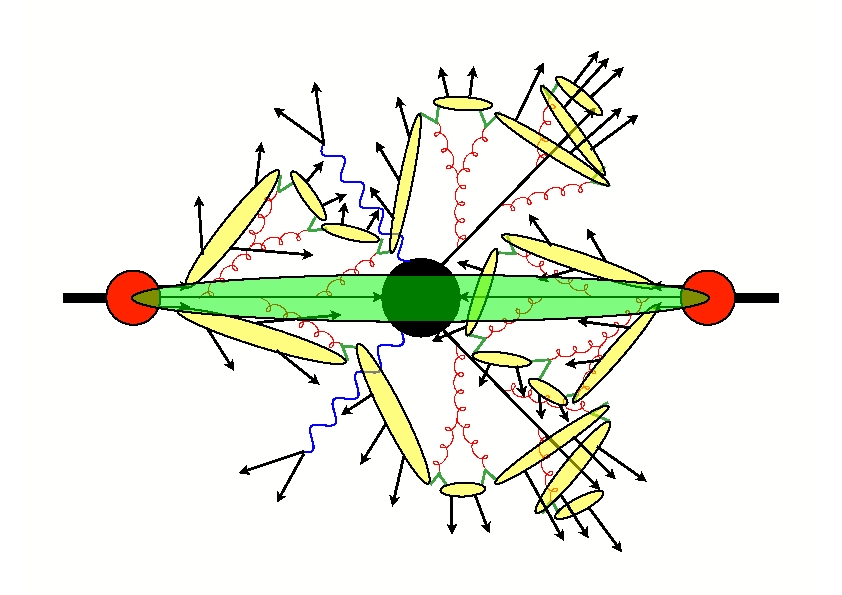
\includegraphics[width=0.55\textwidth]{theory/fig/ps}
    \caption{ A diagram depicting parton showering (additional emissions) and hadronization (formation of colorless hadrons represented as yellow blobs). The original hard process is shown as a black blob in the middle of the picture.}
    \label{fig:theory:ps}
 \end{center}
\end{figure}

\section{Theoretical Predictions}
\label{sec:theory:nnlo}
This section outlines the practical aspects of theoretical predictions used in this analysis. Computationally intensive and requiring careful fine-tuning of the Monte-Carlo programs, these calculations demanded a considerable effort by a dedicated theory team.

Theoretical predictions of hadronic W and Z production cross-sections were calculated to NLO and NNLO QCD using the programs
FEWZ~\cite{Gavin:2010az, Gavin:2012sy, Li:2012wn} and
DYNNLO~\cite{Catani:2007vq,Catani:2009sm}.
These are the only available programs that allow the computation of
NNLO cross-section while applying fiducial kinematic cuts.

The following NNLO PDF families were interfaced with FEWZ and DYNNLO:
\begin{itemize}
\item CT10 NNLO~\cite{Lai:2010vv},
\item ABM11 NNLO~\cite{Alekhin:2012ig},
\item HERAPDF 1.5 NNLO~\cite{Aaron:2009aa,Radescu:2011cn},
\item MSTW2008 NNLO~\cite{Martin:2009iq},
\item NNPDF2.3 NNLO $\alpha_S = 0.118$~\cite{Ball:2012cx}, and
\item JR09 NNLO~\cite{JimenezDelgado:2008hf}.
\end{itemize}

Electroweak parameters were chosen according to the Particle Data Group recommendations~\cite{PDG} and listed in Tab.~\ref{tab:EW parameters}.

\begin{table}[tb]
  \begin{center}
\begin{tabular}{lrlr}
\hline
\hline
    $M_Z$                       & 91.1876 GeV                        & $V_{ud}$      & 0.97427  \\
    $\Gamma_Z$                  & 2.4949 GeV                            & $V_{us}$      & 0.22534  \\
    $\Gamma(Z \rightarrow ll)$  & 0.084 GeV                             & $V_{ub}$      & 0.00351  \\
    $M_W$                       & 80.385 GeV                        & $V_{cd}$      & 0.22520  \\
    $\Gamma_W$                  & 2.0906 GeV                            & $V_{cs}$      & 0.97344  \\
    $\Gamma(W \rightarrow l\nu)$ & 0.22727 GeV                          & $V_{cb}$      & 0.0412   \\
    $M_H$                       & 125     GeV                        & $V_{td}$      & 0.00867  \\
    $m_t$                       & 173.5   GeV                        & $V_{ts}$      & 0.0404   \\
    $G_F$                       & $1.166 \times 10^{-5}$ GeV$^{-2}$ & $V_{tb}$      & 0.999146 \\
    $sin^2\theta_W$             & 0.2229                   &               &       \\
    $\alpha_G$                  & $7.5624 \times 10^{-3}$  &               &       \\
    $vec_{up}$                  & 0.4056                   &               &       \\
    $vec_{dn}$                  & -0.7028                  &               &       \\
    $vec_{le}$                  & -0.1084                  &               &       \\

    \hline
    \hline
    \end{tabular}
    \caption{Electroweak input parameters for evaluation of the $W^-$, $W^+$ and $Z$ cross-sections.}
    \label{tab:EW parameters}
  \end{center}
\end{table}


%5
\chapter{Data and Monte-Carlo Samples}
\label{chap:mc}
% Collision data, MC samples and reweightings
\section{Collision Data}
\label{mc:sec:coldata}

All events that pass the trigger (Sec.~\ref{sec:det:trigger}) are assigned to a data stream, which is saved to disk for further analysis. For example, the ``Egamma'' stream contains events that passed at least one of the electron or photon triggers, while the ``JetEtMiss'' stream contains events with jets or missing transverse energy. An event that contains both a jet and an electron can be saved in both streams. Naturally, this analysis utilizes the ``Muon'' stream, which contains about 440 million events in total.

Data collected throughout 2011 is separated into 11 data periods (B, D-M). A new period is started when significant changes occur in operating conditions (such as the introduction of a new trigger menu), or after a technical shutdown. The transition from period B to period D involved a particularly significant change in conditions: the time spacing between bunch collisions was decreased from 75 ns to 50 ns. Because 50 ns bunch spacing was preserved for the rest of the year, period B with its abnormal bunch spacing was dropped entirely from this analysis, resulting in a small data loss on the order of 0.7\%.

The amount of data collected at collider experiments is described through the concept of luminosity. Instantaneous luminosity measures the flux, which has the units of the number of particles per unit time per unit area: $cm^{-2} s^{-1}$. Integrating the flux over a period of time, we obtain integrated luminosity in units of $cm^{-2}$. However, in order to keep the numbers manageable, high energy physicists use an alternative unit of area: barn. By definition, 1 barn is $10^{-24}~cm^2$, which is approximately equal to the cross-sectional area of uranium. Integrated luminosity is then expressed in units of inverse-barns, usually $fb^{-1}$.

Cross-sections of various processes are expressed in units of area (usually $nb$). Multiplying cross-section by integrated luminosity produces the expected number of process events in a given amount of collected data. 

Fig.~\ref{fig:mc:lumi} shows the total integrated luminosity collected throughout 2011, as a function of the day of the year.

\begin{figure}[phtb]
  \begin{center}
    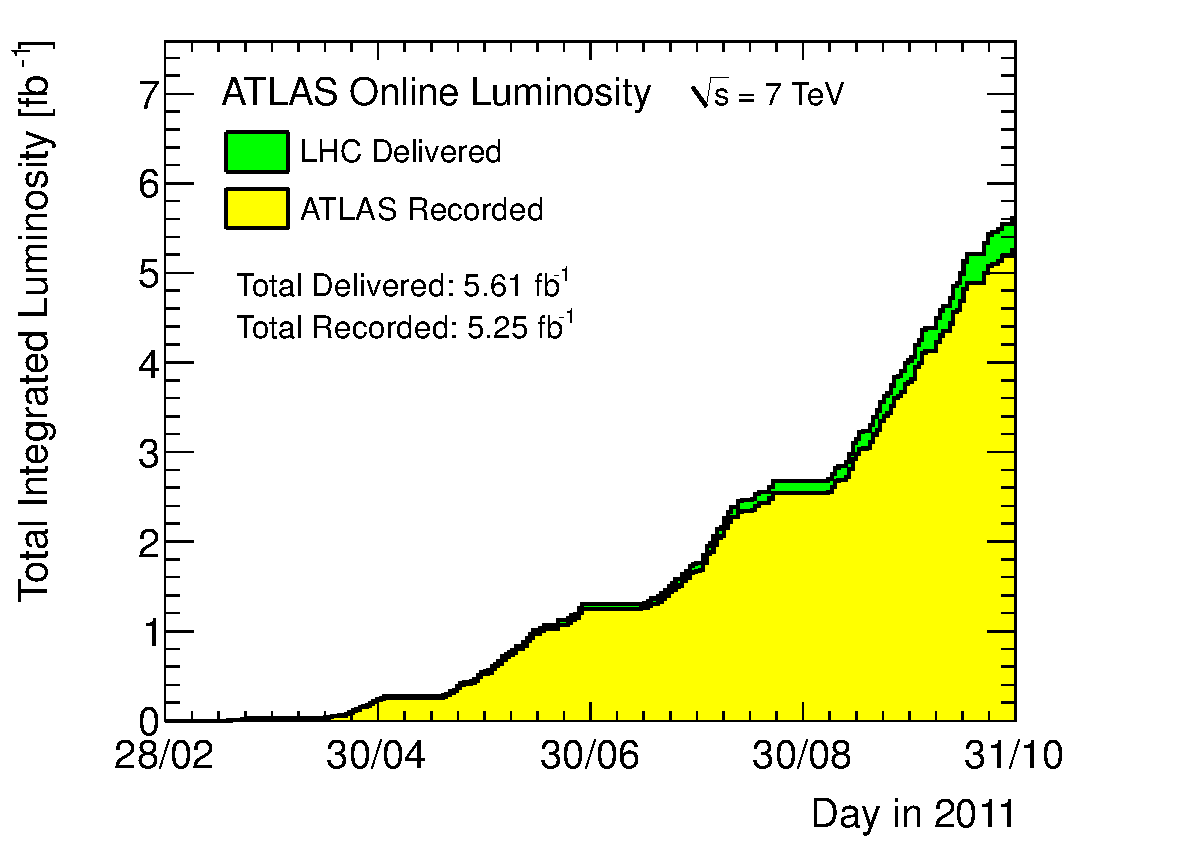
\includegraphics[width=0.7\textwidth]{mc/fig/sumLumiByDay}
    \caption{ Integrated luminosity in 2011 as a function of the day of the year.}
    \label{fig:mc:lumi}
 \end{center}
\end{figure}

The data considered in this analysis has a total integrated luminosity of \lumitr\ with a systematic uncertainty of $1.8\%$~\cite{ATLAS-CONF-2012-080}. The integrated luminosity figure is smaller than the $5.25$ $fb^{-1}$ recorded by ATLAS because data collected in suboptimal conditions was removed from the analysis.

\section{Monte-Carlo Samples}
Monte-Carlo simulation plays a crucial role in this analysis. It serves two purposes: to estimate and subtract the backgrounds to \Wmn\ decay, and to ``unfold'' the measured distributions to a detector-independent cross-section, as outlined in Sec.~\ref{sec:xsec_formula}.

Monte-Carlo events are produced through a series of steps:
\begin{itemize}
\item \textbf{Generation} - creates a list of four-vectors of all stable particles produced in a proton-proton collision. Generators calculate scattering amplitudes, perform parton showering and hadronization, and include the emissions from the underlying event. In the ATLAS simulation framework, the output of all generators is interfaced with two additional programs: \Photos~\cite{Golonka:2005pn}, which simulates the final state QED radiation, and \Tauola~\cite{Jadach:1990mz}, which decays polarized $\tau$ leptons.
\item \textbf{Simulation} - propagates all final state particles through the ATLAS detector using the GEANT4 toolkit~\cite{geant4}, which includes a detailed treatment of the interaction of particles with the material in the detector. GEANT4 relies on a comprehensive model of the detector, which includes everything from bulk material to individual mounting brackets.
\item \textbf{Digitization} - converts the energy depositions left in the detector into digital values seen by the readout electronics. In addition, the effect of multiple proton-proton interactions per bunch crossing (pileup) is simulated by overlaying the so-called minimum bias events on the original hard scattering interaction. Minimum bias events model the average detector response from a typical proton-proton collision, unbiased by resonant processes. LHC run conditions prevalent in 2011 produced around 10 additional pileup interactions per bunch crossing.
\item \textbf{Reconstruction} - takes digitized event data and identifies and reconstructs all particles (muons, jets, et cetera) in the event. Reconstruction software at ATLAS consists of a large collection of packages fine-tuned over the years using test beam studies and the LHC data. The same reconstruction algorithms run on Monte-Carlo simulation and real detector data.
\end{itemize}

Generation is the most interesting step because it is closely related to theory and depends on the modeling of non-perturbative parts of QCD calculations, such as PDFs or parton showers. In this analysis, the following generator programs are used for signal and background samples:

\begin{itemize}
\item \Powheg~(Positive Weight Hardest Emission Generator)~\cite{Nason:2004rx,Frixione:2007vw,Alioli:2008gx,Alioli:2010xd} - an NLO generator used for \Wmn\ and \Zmm\ samples. For parton showering, \Powheg\ can be interfaced with \Pythia~\cite{pythia} or \Herwig~\cite{Corcella:2000bw} programs. \Pythia\ showering is used by default, while \Herwig\ provides a systematic variation.
\item \Mcatnlo~\cite{mcatnlo} - an alternative NLO generator used to produce systematic variations of \Wmn\ and \Zmm\, as well as $t\bar{t}$ and single top samples. Unlike \Powheg, \Mcatnlo\ generates a subset of events with negative weights (about 10\% of the total) that combine with positive-weight events to enforce NLO accuracy. \Mcatnlo\ can be interfaced only with \Herwig\ for showering.
\item \Herwig~\cite{Corcella:2000bw} - a general-purpose generator used both for matrix element calculations and parton showering in diboson samples.
\item \Alpgen~\cite{Mangano:2002ea} - a generator that specializes in multi-parton processes by computing the full matrix element of configurations with additional emissions. It was used for $W\to\tau\nu$ and $\Zg \to \tau\tau$ samples because the more traditional \Pythia-based $\tau$ samples have limited statistics and suffer from incorrect treatment of $\tau$ polarization.
\end{itemize}

All NLO Monte-Carlo samples are interfaced with the \pdfCteq\ PDF set.

\subsection{List of Samples and their Cross-Sections}

Table~\ref{tab:samples} contains a full list of Monte-Carlo samples used in this analysis. For each sample, the table provides its cross-section times the branching ratio times the filter efficiency (pre-selection efficiency at the generator level), and the total number of simulated events.

Electroweak processes are normalized to the NNLO cross-sections computed with the FEWZ program~\cite{Gavin:2010az, Gavin:2012sy, Li:2012wn}. The uncertainty on these cross-sections arises from the choice of PDF (3\%) and factorization and renormalization scales.

\begin{table}[p]
  \small
  \begin{center}
    \begin{tabular}{l|l|r|r}
      \hline
      \hline
      \raisebox{-0.4ex}{Process} & Generator & $\sigma{\cdot}
      \text{BR}{\cdot}\epsilon_{filter}$ [nb] & $N_{evt}\,[10^6]$\\
      \hline\hline

      \multicolumn{3}{c}{Signal samples for \Wln}\\\hline
      \Wplusmunu     &  \Powheg\Pythia  & 6.16 (5\%) & 23 \\
      \Wminusmunu    &  \Powheg\Pythia  & 4.30 (5\%) & 17 \\
      \Wplusmunu     & \Powheg\Herwig   & 6.16 (5\%) & 16 \\
      \Wminusmunu    & \Powheg\Herwig   & 4.30 (5\%) & 12 \\
      \Wplusmunu     & \Mcatnlo & 6.16 (5\%) & 16 \\
      \Wminusmunu    & \Mcatnlo & 4.30 (5\%) & 12 \\

      \hline \multicolumn{3}{c}{\Zgll\ samples}\\\hline
      \Zgll ~~($\mll > 53.8\gev$) &   \Powheg\Pythia   &  1.01 (5\%) & 20\\
      \Zgll ~~($\mll < 53.8\gev$)  &  \Powheg\Pythia   &  0.088 (5\%) & 3\\

      \hline \multicolumn{3}{c}{\Alpgen\Herwig\  and \Sherpa\ \Wln\ and \Zgll\ samples}\\\hline
      \Wtau\ Np0   &   \Alpgen\Herwig\ & 8.29 (5\%) & 3.4 \\
      \Wtau\ Np1   &   \Alpgen\Herwig\ & 1.56 (5\%) & 2.5 \\
      \Wtau\ Np2   &   \Alpgen\Herwig\ & 0.45 (5\%) & 3.8 \\
      \Wtau\ Np3   &   \Alpgen\Herwig\ & 0.12 (5\%) & 1 \\
      \Wtau\ Np4   &   \Alpgen\Herwig\ & 0.03 (5\%) & 0.25 \\
      \Wtau\ Np5   &   \Alpgen\Herwig\ & 0.008 (5\%) & 0.07 \\

      \Ztau\ Np0  &  \Alpgen\Herwig\  & 0.83 (5\%) & 6.6 \\
      \Ztau\ Np1  &  \Alpgen\Herwig\  & 0.17 (5\%) & 1.3 \\
      \Ztau\ Np2  &  \Alpgen\Herwig\  & 0.051 (5\%) & 0.81 \\
      \Ztau\ Np3  &  \Alpgen\Herwig\  & 0.014 (5\%) & 0.22 \\
      \Ztau\ Np4  &  \Alpgen\Herwig\  & 0.004 (5\%) & 0.06 \\
      \Ztau\ Np5  &  \Alpgen\Herwig\  & 0.0009 (5\%) & 0.02 \\

      \hline \multicolumn{3}{c}{$t\bar{t}$ and single top samples}\\\hline
      $t\bar{t}$   & \Mcatnlo & 0.098 (6.2\%) & 1.5\\
      single top, $t$ chan  & \Mcatnlo & $7.12\cdot 10^{-3}$ (12\%) & 0.3\\
      single top, $s$ chan & \Mcatnlo & $0.47\cdot 10^{-3}$ (12\%) & 0.3\\
      single top, $Wt$ chan & \Mcatnlo & $14.59\cdot 10^{-3}$ (12\%) & 0.9\\

      \hline \multicolumn{3}{c}{Diboson samples}\\\hline
      $WW$ & \Herwig & 17.5 $\cdot 10^{-3}$ (7\%) & 1.5 \\
      $WZ$ & \Herwig & 5.7 $\cdot 10^{-3}$ (7\%) & 1 \\
      $ZZ$ & \Herwig & 1.3 $\cdot 10^{-3}$ (7\%) & 0.25 \\

      \hline \multicolumn{3}{c}{QCD samples (for cross-checks only)}\\\hline
      $b\overline{b}$ ($p_{T, \mu} > 15\gev$) & \Pythia & $73.9$ & 4.5\\
      $c\overline{c}$ ($p_{T, \mu} > 15\gev$) & \Pythia & $28.4$ & 1.5\\

      \hline\hline
    \end{tabular}
    \caption{ Monte-Carlo samples used in the analysis. The numbers in the parentheses next to cross-section values indicate the uncertainty on these cross-sections. The quoted cross-sections are the ones used to normalize the estimates of expected Monte-Carlo event counts. }
    \label{tab:samples}
  \end{center}
\end{table}

\section{Theoretical Extrapolation Tables}
\label{sec:mc:extraptables}
The extrapolation (\E) and acceptance (\A) factors (defined in Sec.~\ref{sec:xsec_formula}) are derived from \Wmn\ Monte-Carlo. Four sources of systematic uncertainty are considered when assigning errors to \E\ and \A\ factors:
\begin{itemize}
\item The uncertainty envelope of the default CT10 parton distribution function (PDF) family. PDF's assign a fraction of the total proton momentum to the quarks or gluons that interact to produce a \Wboson\ boson. These distributions are not calculable from first principles and are measured experimentally, mostly from proton-electron scattering experiments. A more detailed discussion is available in the theory section~\ref{chap:pdf_theory}.
\item Variations arising from using alternative NLO (next-to-leading order) PDF families. There are several NLO PDF families maintained by various research groups, each emphasizing different experimental inputs or fitting techniques to derive parton distributions. The maximum deviation between the default CT10 family and one of the following PDF families is taken as the uncertainty:
\begin{itemize}
\item ABM11 NLO~\cite{Alekhin:2012ig}
\item HERAPDF 1.5 NLO~\cite{Aaron:2009aa,Radescu:2011cn}
\item MSTW2008 NLO~\cite{Martin:2009iq}
\item NNPDF2.3~\cite{Ball:2012cx}
\end{itemize}
\item Variations arising from using an alternative Matrix Element (ME) Monte-Carlo generator. Matrix elements involve the ``hard'' (high-$p_{T}$) part of the interaction that can be calculated in perturbative QCD through Feynman diagrams. Differences between Monte-Carlo generators arise in the specific implementation, particularly once these calculations go beyond the leading order. Further details are available in Sec.~\ref{chap:qcd_theory}. The ME uncertainty is taken as the difference between the \Mcatnlo\ and \Powheg\ generators.
\item Variations arising from using alternative Parton Shower (PS) mechanisms in the Monte-Carlo. Parton showering simulates additional emissions from particles produced in the hard scattering, including soft gluon emissions. The PS uncertainty is taken as the difference between \Herwig\ and \Pythia\ showering.
\end{itemize}

Central values and uncertainties on \E\ and \A\ factors and shown in Tables~\ref{tab:ae_w_int}~-~\ref{tab:ae_w_etaptdiff}. These numbers were derived by the inclusive W/Z analysis group.

\begin{table}
  \footnotesize
  \centering
  \begin{tabular}{|c|r|r|r|r|r|r|}
    \hline
    & ~~Value~~
    & ~~$\Delta_\mathrm{CT10} [\%]$~~
    & $\Delta_\mathrm{PDFmax} [\%]$
    & ~~$\Delta_\mathrm{ME} [\%]$~~
    & ~~$\Delta_\mathrm{PS} [\%]$~~
    & ~~$\Delta_\mathrm{tot} [\%]$~~ \\\hline
    \multicolumn{7}{|l|}{\EW\ \Wmn\ fiducial ($|\eta|<2.4$) to fiducial/extrapolated ($|\eta|<2.5$) } \\
    \hline
    $\Wminus$ & $0.9682$ & $0.07$ & $-0.14$ & $-0.01$ & $-0.03$ & $0.16$\\
    $\Wplus$ & $0.9628$ & $0.06$ & $0.06$ & $-0.00$ & $-0.05$ & $0.09$\\
    \hline
    \multicolumn{7}{|l|}{\AW\ \Wmn\ fiducial/extrapolated to total} \\
    \hline
    $\Wminus$ & $0.4488$ & $0.80$ & $-1.60$ & $-0.62$ & $-0.83$ & $2.07$\\
    $\Wplus$ & $0.4645$ & $0.51$ & $1.11$ & $-0.39$ & $-0.80$ & $1.51$\\
    \hline
  \end{tabular}
  \caption{\AW\ and \EW\ factors and their relative uncertainties for the integrated \Wmn\ measurement.}
  \label{tab:ae_w_int}
\end{table}

\begin{table}
  \footnotesize
  \centering
  \begin{tabular}{|c|c|r|r|r|r|r|r|}
    \hline
    $|\eta|_\mathrm{min}$
    & $|\eta|_\mathrm{max}$
    & ~~Value~~
    & ~~$\Delta_\mathrm{CT10} [\%]$~~
    & $\Delta_\mathrm{PDFmax} [\%]$
    & ~~$\Delta_\mathrm{ME} [\%]$~~
    & ~~$\Delta_\mathrm{PS} [\%]$~~
    & ~~$\Delta_\mathrm{tot} [\%]$~~ \\\hline
    \multicolumn{8}{|l|}{\EW\ \Wminusmunu\ fiducial ($|\eta|<2.4$)
      to fiducial/extrapolated ($|\eta|<2.5$)} \\\hline
    $2.18$ & $2.50$ & $0.6982$ & $0.11$ & $-0.29$ & $0.01$ & $-0.00$ & $0.31$\\
    \hline
    \multicolumn{8}{|l|}{\EW\ \Wplusmunu\ fiducial ($|\eta|<2.4$)
      to fiducial/extrapolated ($|\eta|<2.5$)} \\\hline
    $2.18$ & $2.50$ & $0.6976$ & $0.08$ & $0.24$ & $0.07$ & $-0.11$ & $0.29$\\
  \hline
  \end{tabular}
  \caption{\EW\ factors and their relative uncertainties for the 1D $\eta$ differential \Wmn\ measurements. Because \EW\ factors merely extrapolate the measurement from $|\eta|<2.4$ to $|\eta|<2.5$, they are only needed for the most forward measurement bin. }
  \label{tab:ae_w_etadiff2}
\end{table}

\begin{table}
  \footnotesize
  \centering
  \begin{tabular}{|c|c|c|c|r|r|r|r|r|r|}
    \hline
    $|\eta|_\mathrm{min}$
    & $|\eta|_\mathrm{max}$
    & $p_{T, \mathrm{min}}$
    & $p_{T, \mathrm{max}}$
    & ~~Value~~
    & $\Delta_\mathrm{CT10} [\%]$
    & $\Delta_\mathrm{PDFmax} [\%]$
    & $\Delta_\mathrm{ME} [\%]$
    & $\Delta_\mathrm{PS} [\%]$
    & $\Delta_\mathrm{tot} [\%]$ \\\hline
    \multicolumn{10}{|l|}{\EW\ \Wminusmunu\ fiducial ($|\eta|<2.4$)
      to fiducial/extrapolated ($|\eta|<2.5$)} \\\hline
$2.18$ & $2.50$ & $20.0$ & $25.0$ & $0.6929$ & $0.10$ & $0.40$ & $0.30$ & $0.08$ & $0.51$\\
$2.18$ & $2.50$ & $25.0$ & $30.0$ & $0.6946$ & $0.10$ & $0.15$ & $0.13$ & $-0.01$ & $0.23$\\
$2.18$ & $2.50$ & $30.0$ & $35.0$ & $0.6964$ & $0.11$ & $-0.25$ & $-0.18$ & $-0.04$ & $0.33$\\
$2.18$ & $2.50$ & $35.0$ & $40.0$ & $0.6973$ & $0.12$ & $-0.35$ & $-0.07$ & $-0.03$ & $0.37$\\
$2.18$ & $2.50$ & $40.0$ & $45.0$ & $0.6993$ & $0.13$ & $-0.37$ & $0.04$ & $-0.14$ & $0.42$\\
$2.18$ & $2.50$ & $45.0$ & $50.0$ & $0.7041$ & $0.12$ & $-0.37$ & $0.58$ & $0.55$ & $0.89$\\
$2.18$ & $2.50$ & $50.0$ & $120.0$ & $0.7097$ & $0.13$ & $-0.36$ & $0.31$ & $0.25$ & $0.55$\\
  \hline
    \multicolumn{10}{|l|}{\EW\ \Wplusmunu\ fiducial ($|\eta|<2.4$)
      to fiducial/extrapolated ($|\eta|<2.5$)} \\\hline
$2.18$ & $2.50$ & $20.0$ & $25.0$ & $0.7172$ & $0.09$ & $0.36$ & $0.19$ & $-0.04$ & $0.42$\\
$2.18$ & $2.50$ & $25.0$ & $30.0$ & $0.7057$ & $0.09$ & $0.24$ & $0.22$ & $-0.19$ & $0.39$\\
$2.18$ & $2.50$ & $30.0$ & $35.0$ & $0.6971$ & $0.09$ & $0.20$ & $0.09$ & $-0.08$ & $0.25$\\
$2.18$ & $2.50$ & $35.0$ & $40.0$ & $0.6939$ & $0.09$ & $0.26$ & $0.19$ & $-0.03$ & $0.33$\\
$2.18$ & $2.50$ & $40.0$ & $45.0$ & $0.6925$ & $0.09$ & $-0.28$ & $0.04$ & $-0.38$ & $0.48$\\
$2.18$ & $2.50$ & $45.0$ & $50.0$ & $0.7000$ & $0.09$ & $1.08$ & $-0.92$ & $0.25$ & $1.44$\\
$2.18$ & $2.50$ & $50.0$ & $120.0$ & $0.7097$ & $0.09$ & $0.22$ & $-0.64$ & $-0.06$ & $0.68$\\
  \hline
  \end{tabular}
  \caption{\EW\ factors and their relative uncertainties for the 2D $\eta - p_T$ differential \Wmn\ measurement. Because \EW\ factors merely extrapolate the measurement from $|\eta|<2.4$ to $|\eta|<2.5$, they are only needed for the most forward measurement bin. }
  \label{tab:ae_w_etaptdiff}
\end{table}


\section{Monte-Carlo Corrections}
Several corrections are applied to Monte-Carlo samples to improve the modeling of relevant physics processes and detector conditions. Note that the data-driven corrections to muon momentum and reconstruction efficiency are described separately in the section on muon performance (Sec.~\ref{sec:event:muonperf}).

\subsection{Pile-up Reweighting }
% https://twiki.cern.ch/twiki/bin/view/AtlasPublic/LuminosityPublicResults#2011_pp_Collisions
The effect of multiple proton-proton interactions per bunch crossing (pileup) is accounted for in Monte-Carlo at the digitization step. However, the number of minimum-bias events overlaid in digitization does not exactly match the actual data taking conditions. Consequently, a pileup reweighting is applied as a function of $<\mu>$, the mean number of interactions per bunch crossing.
Fig.~\ref{fig:mc:nvtx} shows a comparison of the number of vertices with at least three tracks before and after pileup reweighting. The number of vertices acts as a proxy for the number of interactions because each $pp$ interaction produces a separate vertex that can normally be identified by looking at vertex positions along the $z$ axis. Pileup reweighting markedly improves the data/MC agreement.

\begin{figure}[phtb]
  \begin{center}
        \subfigure[Before pileup reweighting]{%
          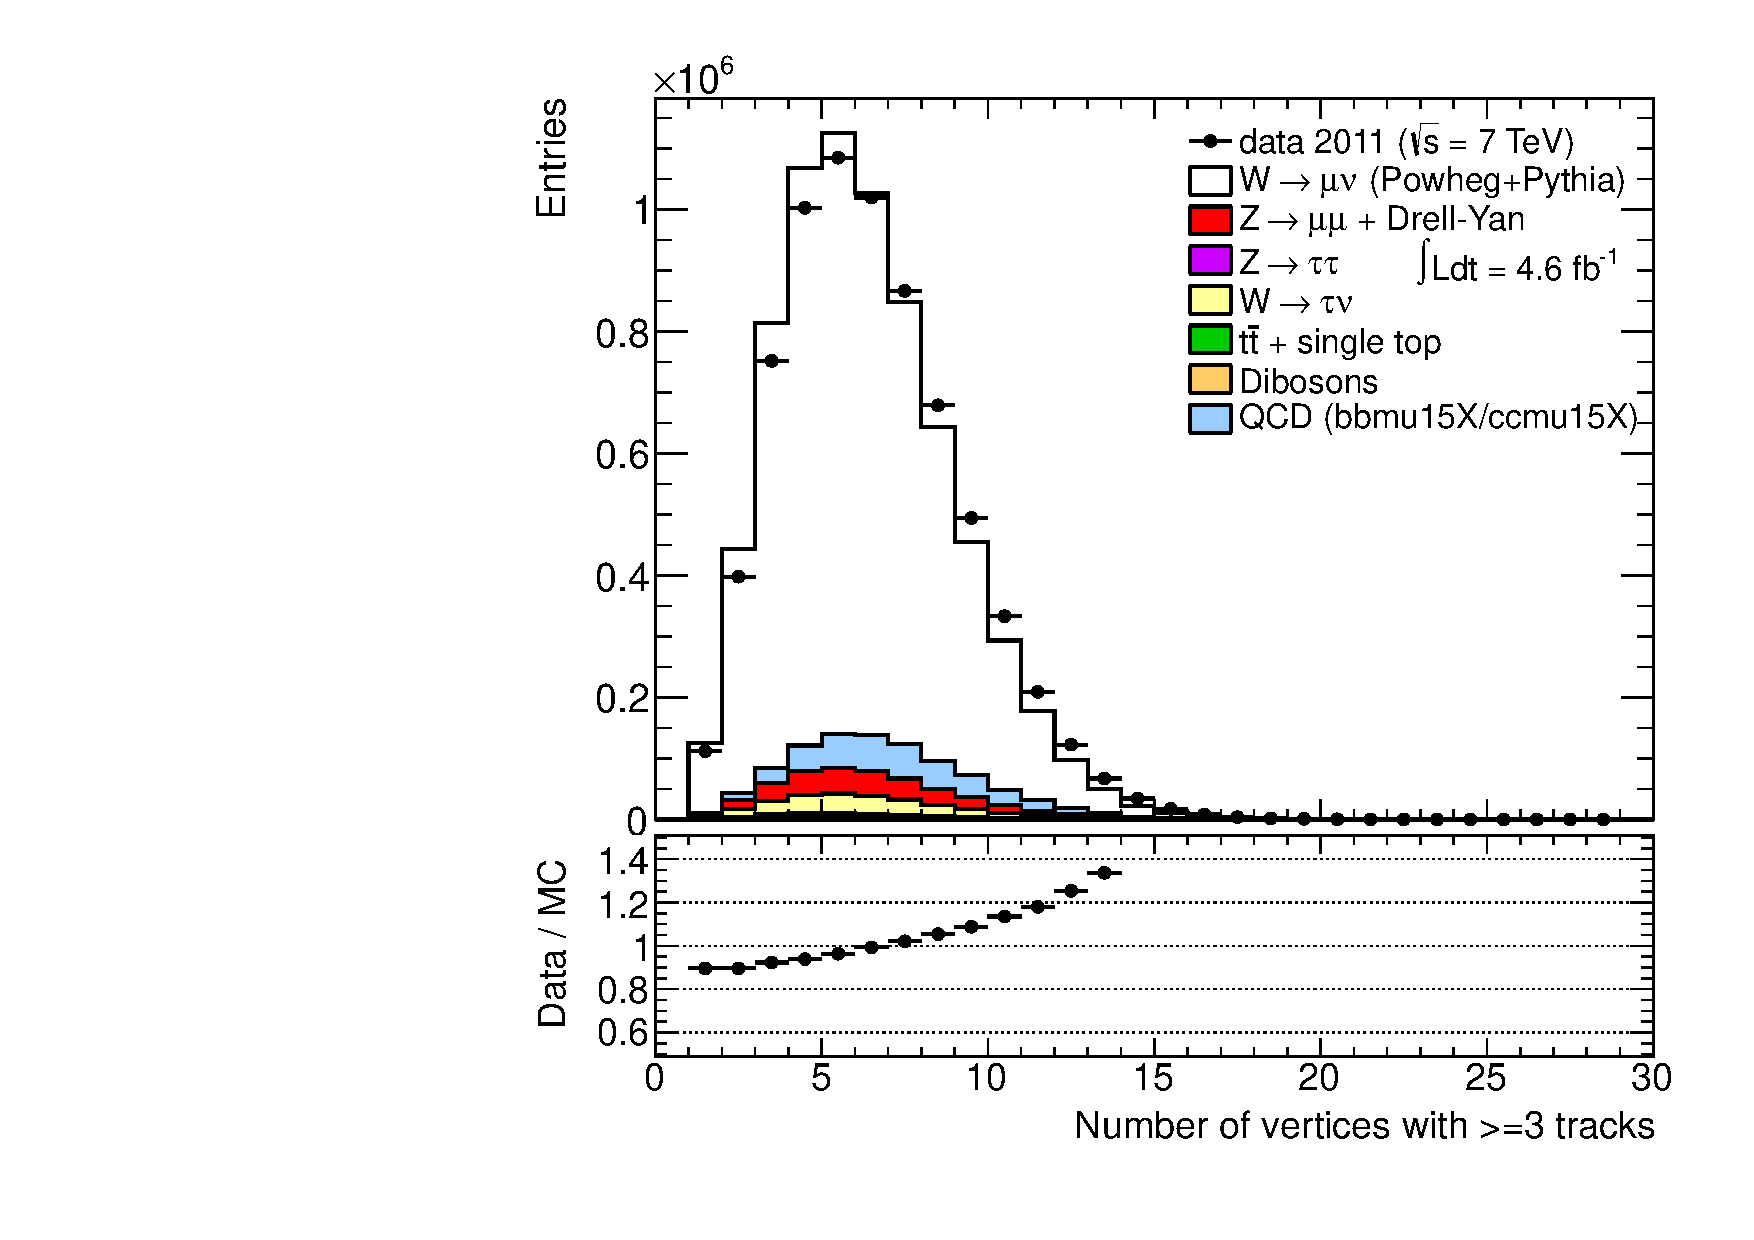
\includegraphics[width=0.44\textwidth]{mc/fig/rw_nvtx_pre}
        } 
        \subfigure[After pileup reweighting]{%
          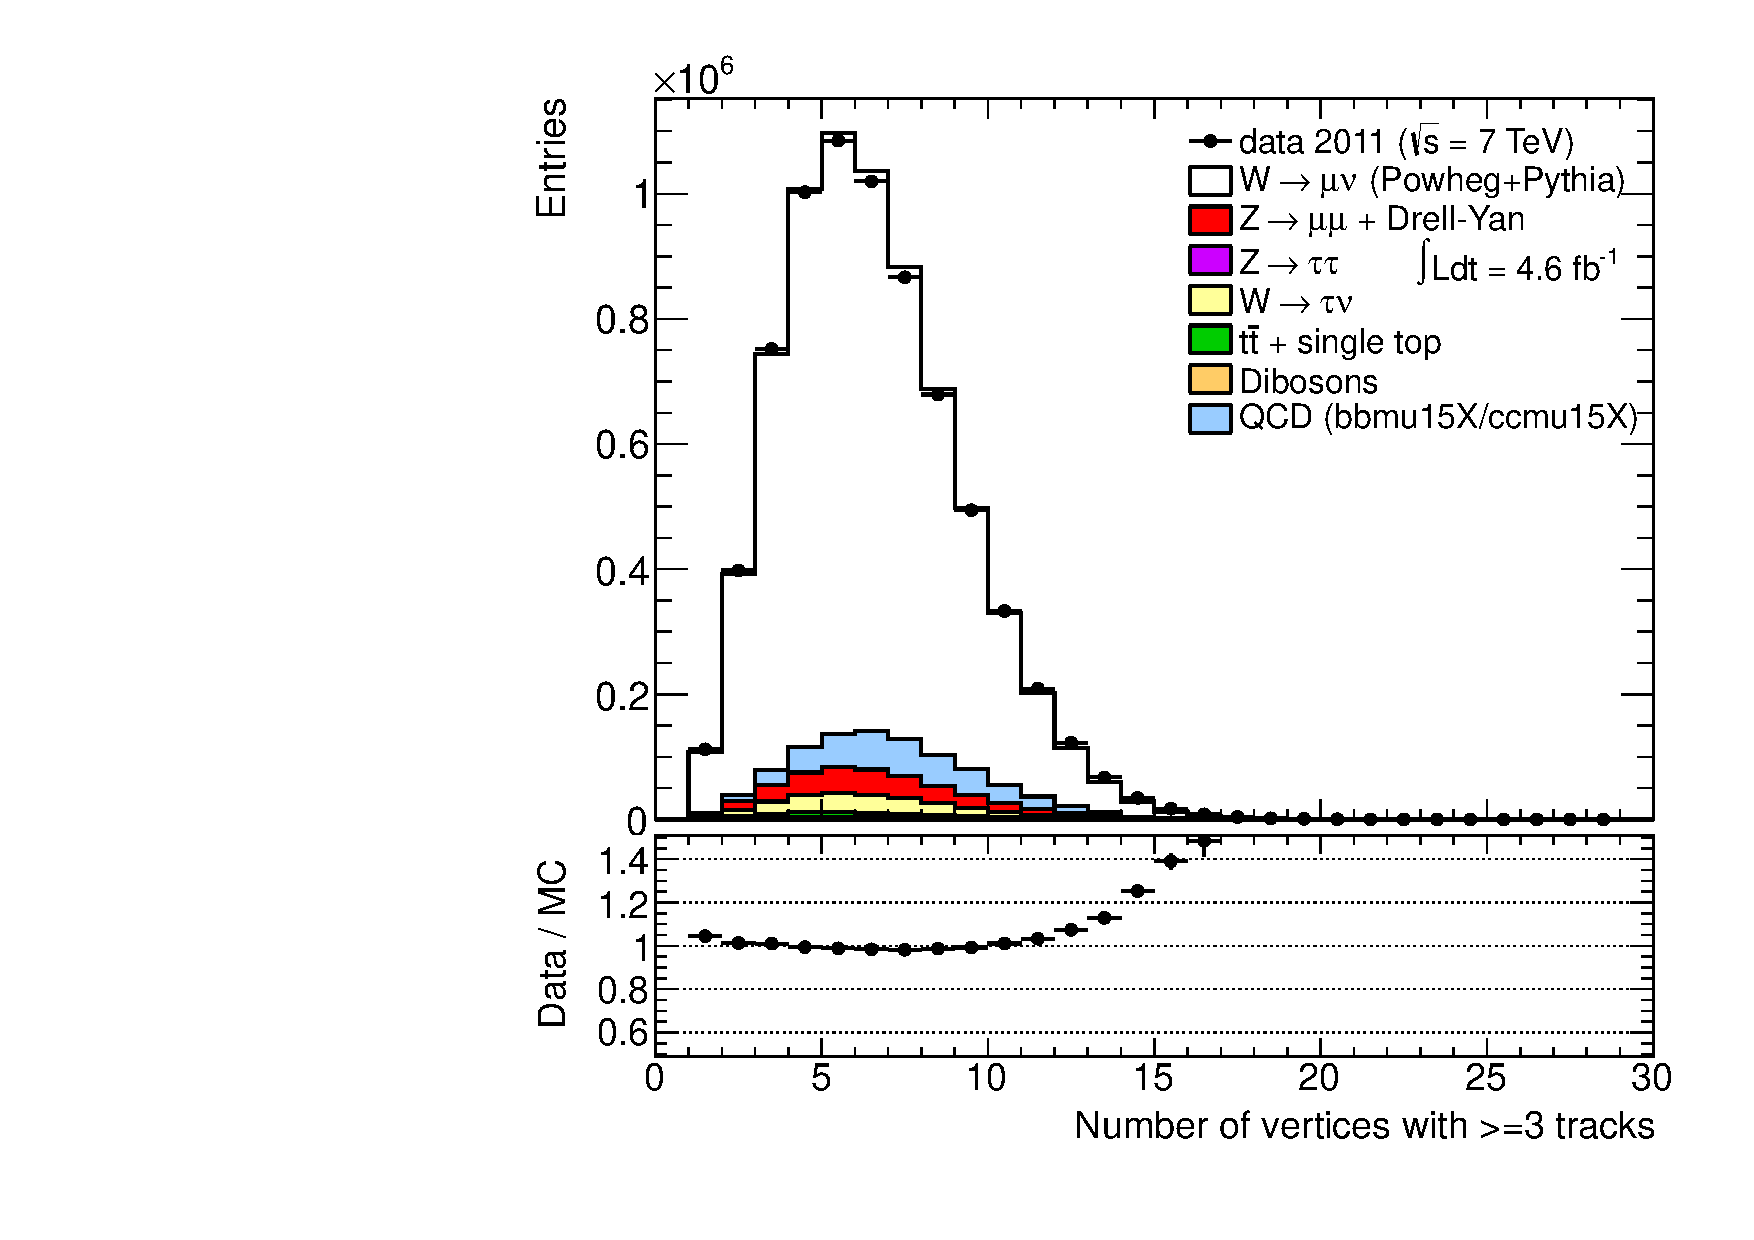
\includegraphics[width=0.44\textwidth]{mc/fig/rw_nvtx_aft}
        }
 \caption{ Distribution of the number of vertices with 3 tracks or more with and without pileup reweighting. Because of residual disagreement even after reweighting, an additional systematic on pileup modeling is introduced in the analysis by scaling the $<\mu>$ distribution by 3\%.}
 \label{fig:mc:nvtx}
 \end{center}
\end{figure}

\subsection{Vertex z Reweighting }
The spread of the beam spot along the $z$ direction is not well modeled in Monte-Carlo. This is corrected by applying a weight to Monte-Carlo at the truth level. Fig.~\ref{fig:mc:vxz0} shows the primary vertex $z_0$ distribution before and after reweighting.

\begin{figure}[phtb]
  \begin{center}
        \subfigure[Before vertex reweighting]{%
          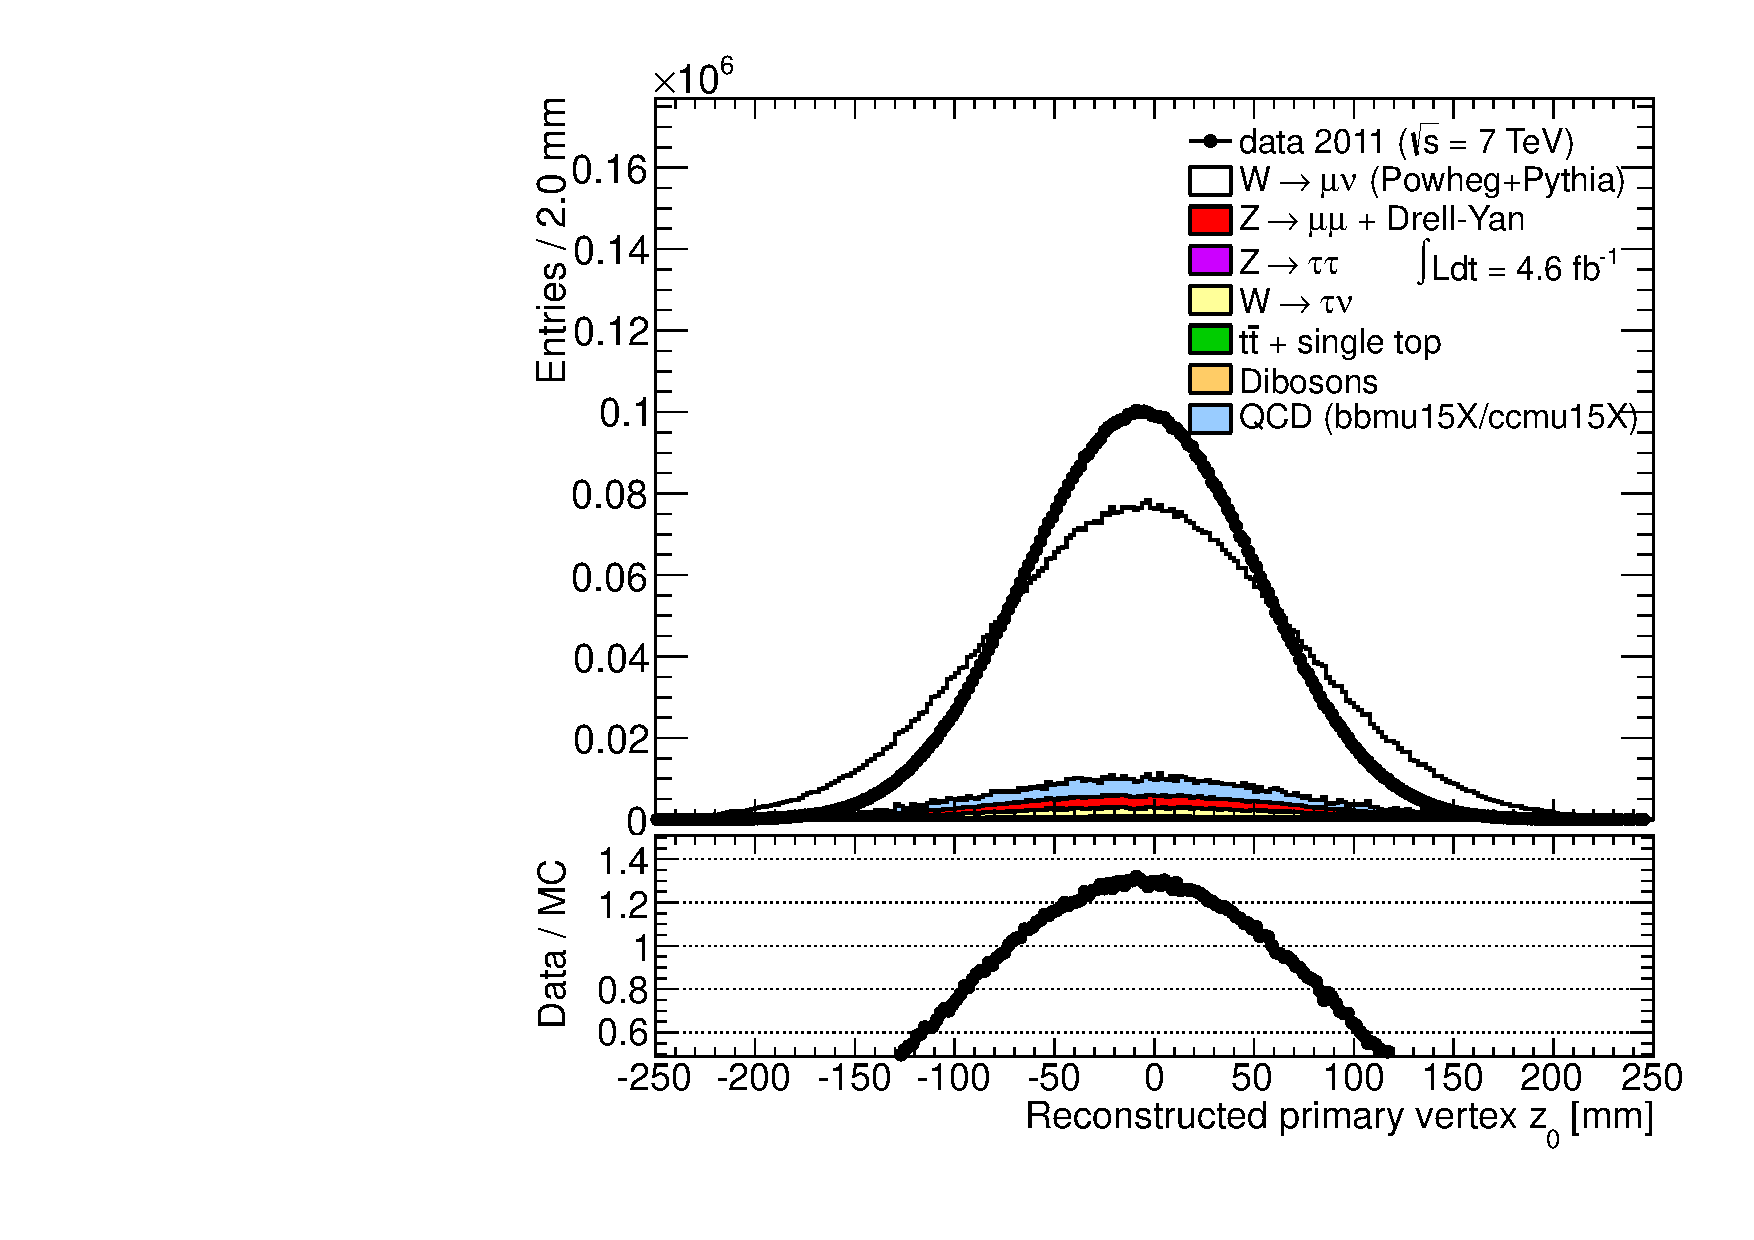
\includegraphics[width=0.44\textwidth]{mc/fig/rw_vxz0_pre}
        } 
        \subfigure[After vertex reweighting]{%
          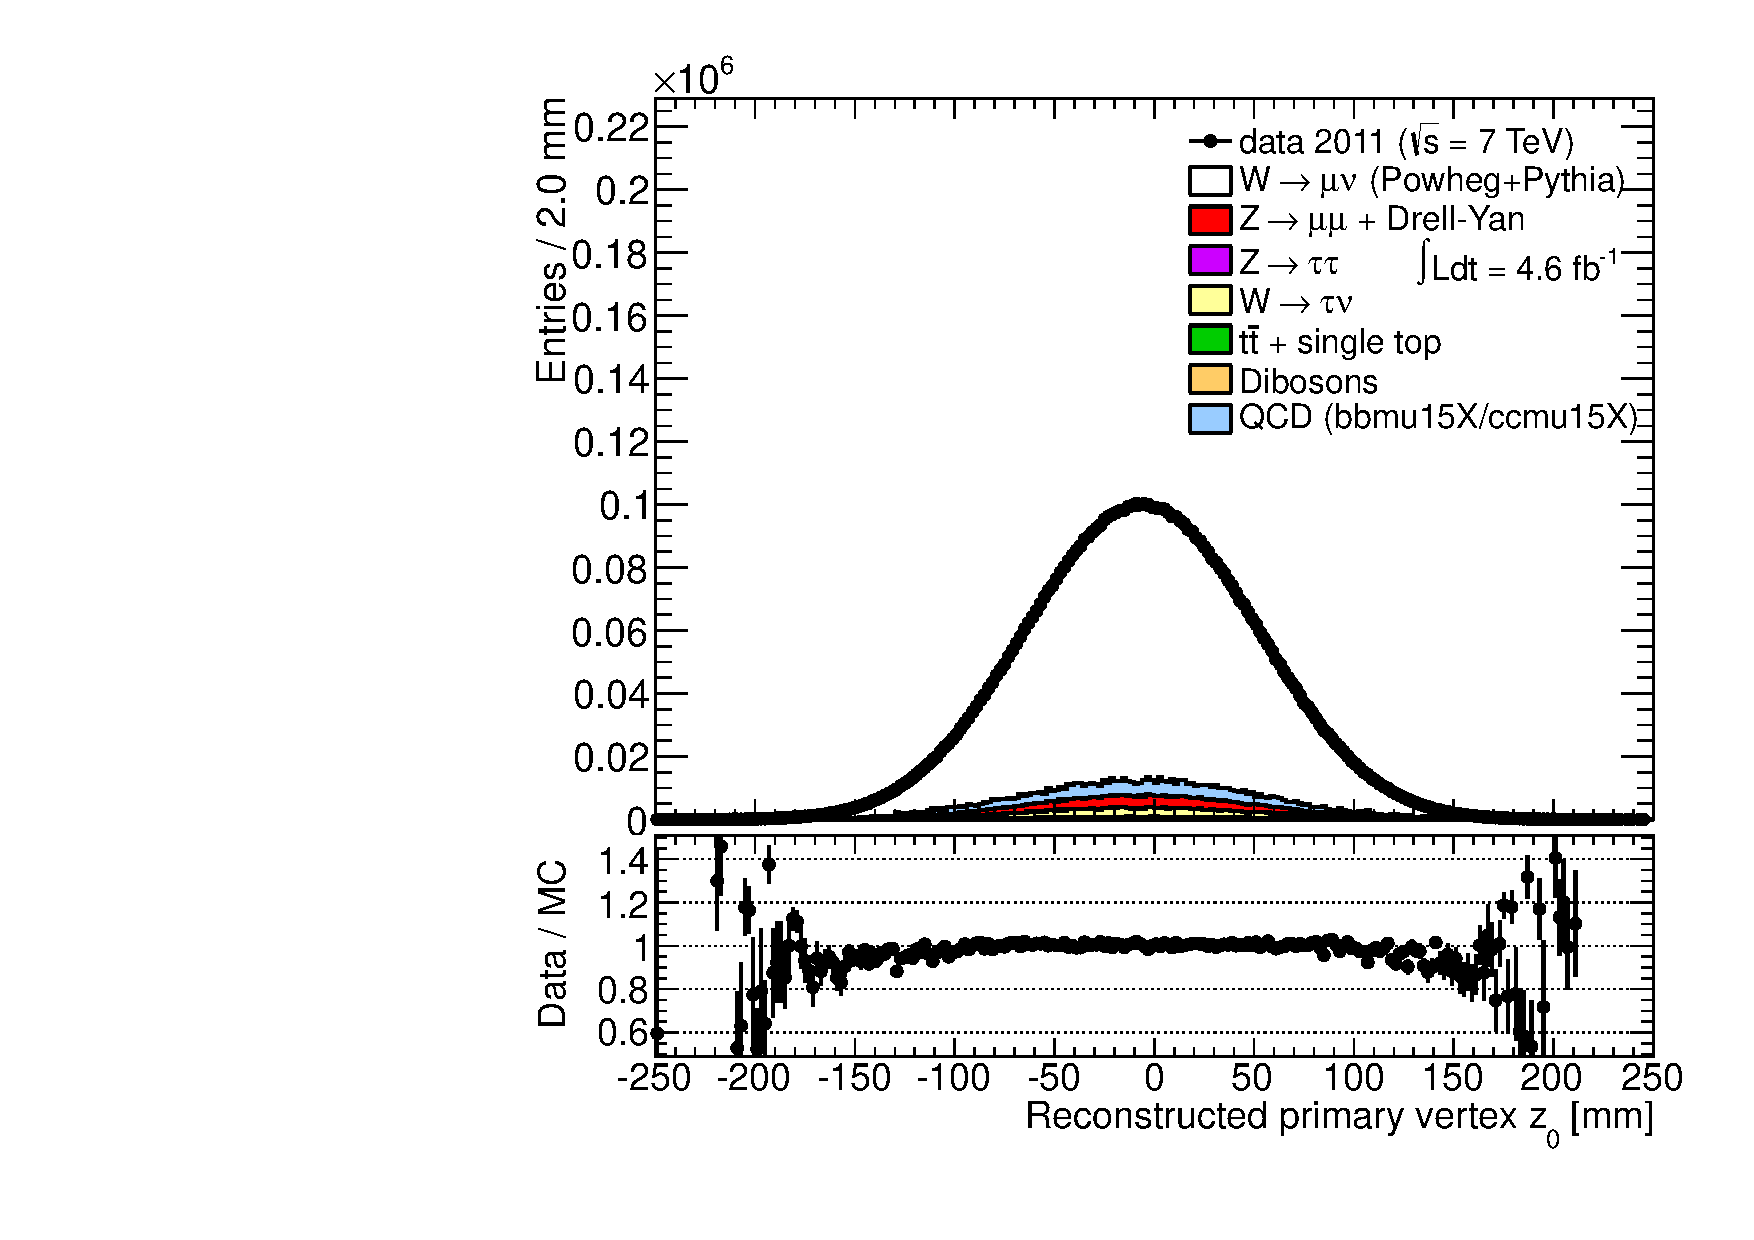
\includegraphics[width=0.44\textwidth]{mc/fig/rw_vxz0_aft}
        }
 \caption{ Primary vertex $z_0$ with and without vertex reweighting. }
 \label{fig:mc:vxz0}
 \end{center}
\end{figure}


\subsection{W and Z $p_T$ Reweighting }
\label{sec:bosonptreweight}
Published ATLAS $Z$ $\phi^*$ and $\pt$ analyses~\cite{Aad:2011fp} suggest that the boson $p_T$ spectrum is not correctly modeled by existing NLO generators. For example, \Fig~\ref{fig:zphistar_mcplot} from~\cite{zphistar} shows that none of the generators attain good data/MC agreement in the $Z$ $\phi^*$ variable, which is highly correlated to boson $p_T$ via $\phi^* \sim p_{T,\ell\ell}/\mll \approx p_{T,\ell\ell}/100\gev$. Therefore, for the nominal measurement, W and Z boson $p_T$ is reweighted in \Powheg\Pythia, \Powheg\Herwig, and \Mcatnlo\ samples to the published Z $p_T$ spectrum~\cite{Aad:2011gj}. The reweighting is based on the measured Z $p_T$ (rather than W $p_T$) because of concerns about hadronic recoil in the W case. Reweighting to \Sherpa\ and \Powheg\Pythiaeight\ is used to assess the systematic uncertainty.

\begin{figure}[htb]
  \begin{center}
    \includegraphics[width=0.9\textwidth]{MCReweights/zphistar_fig_03}
    \caption{Comparison of different MC generators to the $Z$ $\phi^*$ measurement using 2011 ATLAS data.}
    \label{fig:zphistar_mcplot}
  \end{center}
\end{figure}

\subsection{W and Z Lineshape Reweighting }
Generators used to produce \Wln\ and \Zgll\ samples differ in some of their settings, such as the mass and width of the gauge bosons, the form of the resonance parametrization, and the choice of couplings. A set of weights was developed~\cite{iba_maarten_vicini} to reweight each generator to a more optimal ``Improved Born Approximation''. For example, Fig.~\ref{fig:bosonm_reweight} demonstrates that the Z lineshapes of two different Monte-Carlo generators can be brought to a good agreement following the reweighting.

\begin{figure}[htb]
  \begin{center}
    \subfigure[Before \Zgll\ LineShape Reweight]{%
      \includegraphics[width=0.45\textwidth]{MCReweights/zgamma_pythia_powheg_std}
    }%
    \subfigure[After \Zgll\ LineShape Reweight]{%
      \includegraphics[width=0.45\textwidth]{MCReweights/zgamma_pythia_powheg_rew}
    } \\
    \caption{Effect of lineshape reweighting on the ratio of \Pythia\ and \Powheg\Pythia. Agreement is achieved following reweighting to the ``Improved Born Approximation'' set of parameters. In this particular case, most of the improvement comes from the \Powheg\Pythia\ side.}
    \label{fig:bosonm_reweight}
  \end{center}
\end{figure}

%% \subsection{Alpgen Angular Reweighting }
%% \Alpgen\Herwig\ $W\to\tau\nu$ and $\Zg\to\tau\tau$ samples do not model boson rapidity $y$ well due to the fact that they rely on a sub-optimal leading-order PDF (\pdfCteql). The weights are derived by comparing the nominal samples with samples reweighted to \pdfCteq.

\subsection{PDF reweighting}

The authors of PDF families provide uncertainties on the fitted momentum fractions through a set of PDF ``members'' that deviate from the nominal PDF by moving along error eigenvectors. For example, the CT10 family contains 52 members, making it impractical to re-run the full Monte-Carlo chain for each member.
As an alternative, PDF reweighting is applied to the nominal Monte-Carlo samples. For each event, the information stored in the truth record is used to calculate the weight via:
\begin{equation}
  w = \frac{xf_1^\mathrm{new}(x_1, Q^2_1) xf_2^\mathrm{new}(x_2, Q^2_2) }{xf_1^\mathrm{old}(x_1, Q^2_1) xf_2^\mathrm{old}(x_2, Q^2_2)}\,
\end{equation}
where $xf_i^\mathrm{new(old)}(x,Q^2)$ are the PDFs of the incoming
parton $i$ evaluated at a given Bjorken $x$ and scale $Q^2$ of the new
(old) PDF set~\cite{Bourilkov:2006cj}.
PDF reweighting is facilitated through the LHAPDF package~\cite{Whalley:2005nh}.


%6
\chapter{Object Reconstruction}
\label{chap:perf}
% performance

This chapter outlines the algorithms that reconstruct muons and evaluate the missing transverse energy. Furthermore, it describes the data-driven corrections that were applied to muons in Monte-Carlo to correct for defects that are not modeled in the simulation. These corrections are derived from \Zmm\ events, which serve as a standard candle in the tag-and-probe procedure.

\section{Muon Reconstruction}
\label{sec:event:muonperf}

\subsection{Trigger}
\label{sec:event:trig}
In order to select events with muons, ATLAS deploys several muon triggers that differ in the $p_T$ threshold, muon multiplicity in the final state, and underlying implementation. Muon candidates are first defined in the hardware-based Level-1 (L1) trigger, where coincidental hits within narrow Regions of Interest (ROI) are detected in RPC and TGC chambers (see Sec.~\ref{chap:det:id}). The L2 trigger refines these muon candidates by adding fine-grained information from MDT and CSC chambers, as well as the hits from the Inner Detector, that are contained within the ROI's. These refinements allow muons from cosmic rays and in-flight meson decays to be rejected. Finally, the Event Filter (EF) trigger has access to the full event data and performs nearly offline-quality reconstruction.

This analysis uses the lowest-$p_T$ unprescaled single-muon triggers. An unprescaled trigger is a trigger with a sufficiently high $p_T$ threshold (and therefore, low firing rate) that it is possible to save every event candidate that fires the trigger. For 2011 data, EF\_mu18 and EF\_mu18\_MG triggers were considered for data taking periods D-I, while EF\_mu18\_medium and EF\_mu18\_MG\_medium were considered for periods J-M. EF\_mu18 and EF\_mu18\_MG trigger chains are seeded by L1\_MU10 ROI's, which require coincidence in two muon spectrometer stations in detecting a $p_T>10$ GeV muon. The ``medium'' chains, owing to increased instantaneous luminosity, are seeded by L1\_MU11, which requires coincidence in three stations for $p_T>11$ GeV muons. Other than the L1 seed, the default and ``medium'' chains are exactly the same at the L2 and EF. ``MG'' stands for MuGirl - one of two muon reconstructions algorithms in ATLAS; triggers without ``MG'' in their name utilize the alternative Muid algorithm. Studies summarized in Appendix~\ref{appendix:ac} motivate the choice of the Muid version of the triggers in the nominal analysis.

All of EF\_mu18 triggers are designed to efficiently detect muons with $p_T >$ 18 GeV, leaving a $2$ GeV buffer zone before the lowest muon $p_T$ cut used in the analysis ($20$ GeV).

%% Fig.~\ref{fig:perf:plato} shows a typical trigger turn-on curve 

%% \begin{figure}[phtb]
%%   \begin{center}
%%     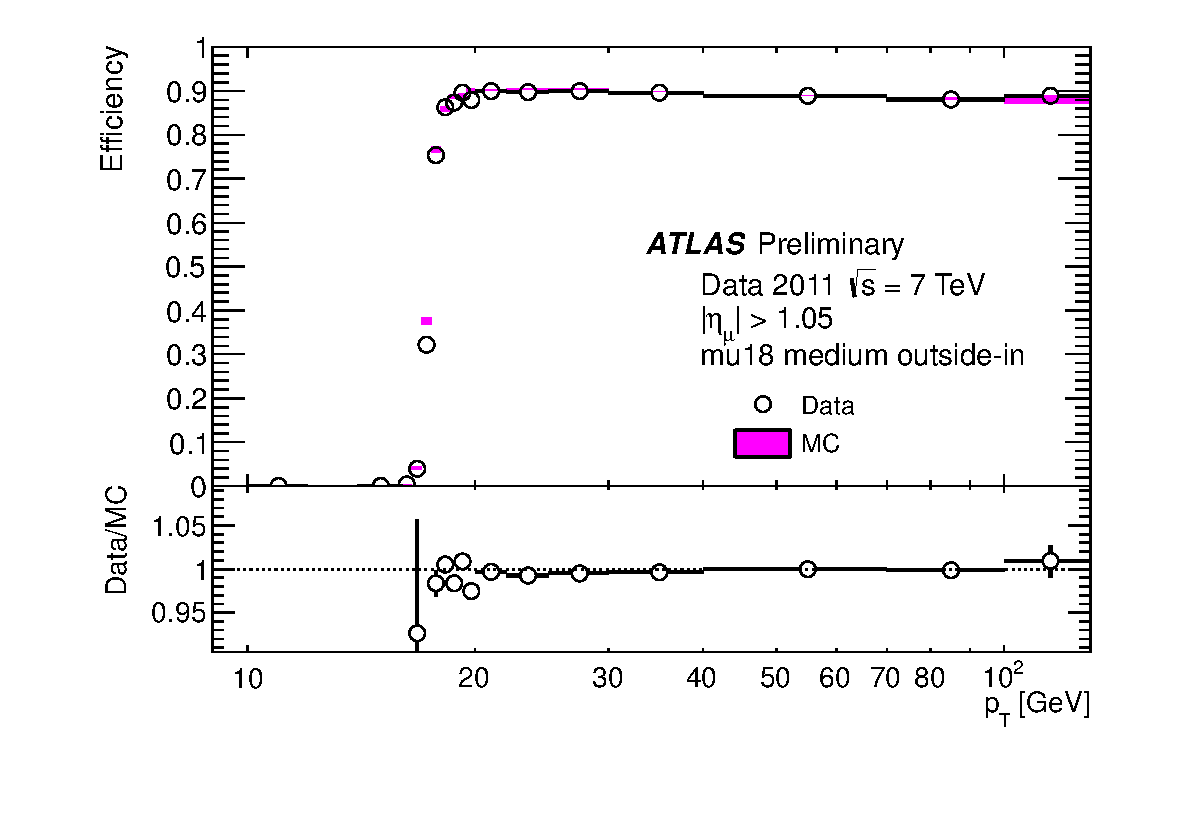
\includegraphics[width=0.70\textwidth]{perf/fig/mu18_turnon}
%%     \caption{ Trigger efficiency of mu18 triggers as a function of muon $p_T$. The trigger reaches its plateau before $p_T = 20~GeV$. }
%%     \label{fig:perf:plato}
%%   \end{center}
%% \end{figure}

\subsection{Muon Types}
Muons are reconstructed as tracks in the Inner Detector (Chap.~\ref{chap:det:id}) and ``Standalone'' muon candidates in the Muon Spectrometer (Chap.~\ref{chap:det:ms}). For high-precision analyses, such as the \Wmn\ cross-section measurement, the two measurements are combined to achieve the highest-quality of muon reconstruction and the best fake-muon rejection.

\paragraph{Inner Detector Tracks}
A typical inner detector track is reconstructed from 3 pixel hits, 8 SCT hits, and 30 TRT hits. The default reconstruction strategy is the ``inside-out'' strategy, which consists of the following steps~\cite{ATLAS-CONF-2012-042}:
\begin{itemize}
\item Three-dimensional spacepoints are formed from pixel and SCT hits.
\item Using pattern recognition, track seeds made of at least three spacepoints are formed.
\item A statistical algorithm called Kalman filter iteratively adds additional hits to the tracks while working outwards.
\item Track candidates are assigned a score based on the number of hits and holes. Low-quality and duplicate candidates are removed.
\item Surviving candidates are extrapolated into TRT. Tracks are re-fitted including TRT hits in the extrapolation region.
\item If the addition of TRT hits results in a lower track score, or if the extrapolation region is not instrumented with TRT modules, the original pixel+SCT track is retained.
\end{itemize}

\paragraph{Standalone Muons}
Standalone muons are constructed by recognizing consistent straight segments within at least two muon chambers that point to the center of the ATLAS detector. Two alternative algorithms are available: Muonboy and MOORE. Muonboy combines track segments through an iterative fitting procedure working outside-in, while MOORE is based on the Hough transform~\cite{leroy2010astroparticle}. Both algorithms extrapolate reconstructed muons to the Inner Detector, with Muonboy parametrizing calorimeter losses as a function of $\eta$ and $p_T$. MOORE supplements the parametrization with actual calorimeter measurements.

\paragraph{Combined Muons}
Standalone muons extrapolated to the Inner Detector are matched to ID tracks through a statistical combination of track parameters and covariances. Those candidates that pass the combination $\chi^2$ cuts are saved in the list of combined muons. Typically, the ID measurement dominates for muons with $p_T<40$ GeV, while more energetic muons are better constrained by the spectrometer.

As in the case of standalone muons, two algorithms exist for muon combination~\cite{muon_tdr}. The STACO algorithm uses MuonBoy candidates and obtains the helix parameters of a combined muon through a statistical combination with the ID track candidate, using the full correlation matrix. The MuId algorithm relies on MOORE standalone candidates and performs a full re-fit of the track including the inner detector hits.

The overall performance of the two algorithms is comparable, and both remain in use. This analysis relies on the STACO reconstruction chain and utilizes isolated STACO muons with additional track quality criteria to reconstruct \Wboson\ bosons (see Sec.~\ref{sec:event:fullsel}).

\section{Muon Corrections}
\label{sec:perf:muoncorr}

Simulating the passage of muons through the ATLAS detector is a complex task. Although test beam studies, cosmic ray calibrations, and studies of earlier collisions have produced an excellent detector model, the Monte-Carlo still suffers from a number of subleading effects, such as unaccounted inhomogeneities in the magnetic field, incorrect material distributions, subtle misalignments, or improperly modeled detector response. For a precision analysis, such as this one, these defects can doom the entire measurement.

Thankfully, nature provides a standard candle - the Z boson - that can be exploited to derive data-driven corrections that bring the efficiency of various cuts in data and Monte-Carlo into agreement. The procedure is commonly known as tag-and-probe, and relies on the correlation between the two muons in \Zmm\ decays. One muon is ``tagged'' with tight requirements, while the second one, called the ``probe'', is initially selected with all cuts minus the one that's under study - such as the requirement that the probe fired a trigger. Z selection is then applied to strongly correlate the two muons. This includes a tight cut on the invariant mass of the muon pair, as well as the requirement that the muons carry opposite charges. This ensures that even the loosely selected probes represent actual muons, as opposed to other objects mis-identified as muons. As the final step, the cut under study (e.g., trigger match) is applied to the probe. Distributions of kinematic variables ($\eta$, $p_T$, etc) of the probe before and after the final cut serve as the denominator and numerator of the efficiency ratio for that cut.

The procedure is separately repeated for data and uncorrected Monte-Carlo. The ratio of their respective efficiencies is a multiplicative scale factor. This scale factor is computed on a per-muon basis and applied to the Monte-Carlo event weight in the nominal analysis.

\subsection{Reconstruction Efficiency}
Reconstruction efficiency scale factors are derived from a standard tag-and-probe procedure, where the probe is either an Inner Detector (ID) track or a so-called CaloTag muon (an ID track with muon-like depositions in the calorimeter). These scale factors correct the combined efficiency of finding a muon candidate in the spectrometer and successfully matching it to the ID track.

Reconstruction scale factors are binned in ($q,\eta,\phi$). $\eta$ binning is chosen to match cross-section binning in the single and double-differential measurements. The scale factors generally stay within 1-2\% of 1, except for narrow $\eta$ regions at the interface between the Barrel and the Endcap, as illustrated in Fig.~\ref{fig:perf:recosf_sf}.

Systematic uncertainty is driven by two sources: choice of the probe, shown in Fig.~\ref{fig:perf:recosf_caloid}, and missing $p_T$-dependence (typically 0.1-0.2\%).

\begin{figure}[phtb]
  \begin{center}
  \includegraphics[width=1.0\textwidth]{MuonPerformance/figures/NewRecoSF/SF_etaPhi_negq}
 \caption{ Reconstruction scale factors for combined STACO muons, which are derived from Z tag-and-probe using ID tracks as probes.}
 \label{fig:perf:recosf_sf}
 \end{center}
\end{figure}

\begin{figure}[phtb]
  \begin{center}
 \includegraphics[width=1.0\textwidth]{MuonPerformance/figures/NewRecoSF/CaloDeviation_etaPhi_negq}
 \caption{ The difference in reconstruction scale factors when using CaloTag vs ID track probes, which contributes to the systematic uncertainty. }
 \label{fig:perf:recosf_caloid}
 \end{center}
\end{figure}

%% \begin{figure}[phtb]
%%   \begin{center}
%%         \subfigure[Reco. SF (nominal)]{%
%%           \includegraphics[width=0.85\textwidth]{MuonPerformance/figures/NewRecoSF/SF_etaPhi_negq}
%%         }
%%         \subfigure[ID track vs CaloTag as probe]{%
%%           \includegraphics[width=0.85\textwidth]{MuonPerformance/figures/NewRecoSF/CaloDeviation_etaPhi_negq}
%%         }
%%  \caption{ Top: reconstruction scale factors for combined STACO muons derived from Z tag-and-probe using ID tracks as probes. Bottom: difference in reconstruction scale factors when using CaloTag vs ID track probes, which contributes to the systematic uncertainty.}
%%  \label{fig:perf:recosf_sum}
%%  \end{center}
%% \end{figure}

%% \begin{figure}[phtb]
%%   \begin{center}
%%         \subfigure[Reco. SF: $\mu^-$]{%
%%           \includegraphics[width=0.44\textwidth]{MuonPerformance/figures/NewRecoSF/SF_etaPhi_negq}
%%         } 
%%         \subfigure[Reco. SF: $\mu^+$]{%
%%           \includegraphics[width=0.44\textwidth]{MuonPerformance/figures/NewRecoSF/SF_etaPhi_posq}
%%         }
%%  \caption{ Reconstruction scale factors for combined STACO muons. These scale factors were derived from Z tag-and-probe using ID tracks as probes.}
%%  \label{fig:perf:recosf}
%%  \end{center}
%% \end{figure}

%% \begin{figure}[phtb]
%%   \begin{center}
%%         \subfigure[ $\mu^-$]{%
%%           \includegraphics[width=0.44\textwidth]{MuonPerformance/figures/NewRecoSF/CaloDeviation_etaPhi_negq}
%%         } 
%%         \subfigure[ $\mu^+$]{%
%%           \includegraphics[width=0.44\textwidth]{MuonPerformance/figures/NewRecoSF/CaloDeviation_etaPhi_posq}
%%         }
%%  \caption{ Difference in reconstruction scale factors when using CaloTag vs ID track probes. This difference contributes to the systematic uncertainty.}
%%  \label{fig:perf:recosf_caloid}
%%  \end{center}
%% \end{figure}

\subsection{Isolation Efficiency}

The definition and motivation behind the muon isolation cut is described in Sec.~\ref{subsec:MuonIsolation}.

Isolation scale factors are derived from Z tag-and-probe events and correct the efficiency of the isolation cut in Monte-Carlo. Isolation scale factors are binned in $p_T$ only, since they were found to be flat in other variables (Fig.~\ref{fig:perf:isosf}). Systematic uncertainty is derived by varying Z tag-and-probe selection cuts by $\pm 10\%$ and adding significant variations in quadrature. The typical uncertainty is 0.1\%.

\begin{figure}[phtb]
  \begin{center}
        \subfigure[Isolation SF: $\eta$]{%
          \includegraphics[width=0.44\textwidth]{MuonPerformance/figures/eff_cb_isoid40rel01_mu_probe_eta}
        } 
        \subfigure[Isolation SF: $p_T$]{%
          \includegraphics[width=0.44\textwidth]{MuonPerformance/figures/eff_cb_isoid40rel01_mu_probe_pt}
        }
 \caption{ Isolation scale factors for the $\frac{p_T^\mathrm{cone40}}{p_T^{\mu}} < 0.1$ cut used in the analysis.}
 \label{fig:perf:isosf}
 \end{center}
\end{figure}

\subsection{Trigger Efficiency}
Trigger scale factors are derived from Z tag-and-probe events, where the probe is required to explicitly match to one of Event Filter trigger objects in a $\Delta R < 0.1$ cone.

Trigger scale factors are binned in ($\eta,p_T,q$), where both $\eta$ and $p_T$ match the binning used in the single and double-differential measurements. The scale factors are computed separately for several data period sub-ranges in order to account for different runtime trigger configurations throughout 2011. Trigger scale factors generally stay within 5\% of 1, but in some pathological cases (Fig.~\ref{fig:perf:trigsf}) may reach 30\%.

Systematic uncertainty is driven by the the lack of $\phi$ parametrization, which could not be added due to insufficient tag-and-probe statistics in the period sub-ranges. This systematic is typically 0.1-0.3\%.

\begin{figure}[phtb]
  \begin{center}
        \subfigure[Trigger SF: $\mu^-$, periods G-I]{%
          \includegraphics[width=0.85\textwidth]{MuonPerformance/figures/scaleFactors/mu18_neg_SF_eta_pt}
        }
        \subfigure[Reco SF: $\mu^+$, periods L3-L4]{%
          \includegraphics[width=0.85\textwidth]{MuonPerformance/figures/scaleFactors/rpc_pos_SF_eta_pt}
        }
 \caption{ Trigger scale factors for mu18 Muid triggers, derived from Z tag-and-probe events. The plot on the right shows the effect of a known RPC misconfiguration in periods L3 and L4, which resulted in large trigger inefficiency in data. }
 \label{fig:perf:trigsf}
 \end{center}
\end{figure}

\subsection{Momentum Resolution and Scale}
\label{perf:muon:scale}
In addition to scale factors to correct Monte-Carlo efficiency of various cuts, a separate correction is needed for the muon momentum.

Muon momentum resolution corrections are derived from \Zmm\ events and curvature differences between ID and spectrometer muons, using the fitting procedure described in~\cite{Cerutti:1322424}. The corrections are derived separately for ID and standalone muon and then propagated to combined muons.

In addition to these resolution terms, corrections are applied to the transverse momentum of the muons
in Monte-Carlo events to improve their agreement with the data. This is necessary to correct the bias
in muon momentum in 2011 Monte-Carlo due to an incorrect multiple scattering model (``Wentzel'') in the Geant4 simulation.
Additionally, these corrections take into account any remaining muon momentum mismodeling due to
detector and magnetic field effects that are not already covered by the resolution corrections.

First, the overall momentum scale (``K'') is set based on the location of the \Zmm\ peak in data and Monte-Carlo.
The uncertainty on the overall momentum scale is derived by varying the cuts used in the \Zmm\ selection, 
and by considering either a full analytic lineshape fit or an iterative Gaussian fit in the core of the invariant mass spectrum~\cite{Kapliy:1358186}.
Second, the component of muon momentum that's anti-correlated between charges (curvature ``C'') is corrected by balancing
positive and negative muons against each other in \Zmm\ events in data. The uncertainty on the curvature correction is
similarly derived by varying the cuts used in the \Zmm\ selection, and by employing two different methods to compute
the corrections (one based on a binned $\chi^{2}$ fit, and another based on unbinned Kolmogorov-Smirnov statistic).

The precise definition of these muon momentum correction parameters is shown below, where it is assumed that all momenta are given in GeV:
$$K \equiv \frac{M_{Z}^{data}}{M_{Z}^{MC}} \approx \frac{p_{T}^{measured}}{p_{T}^{corrected}}$$
$$\frac{1}{p_{T}^{corrected}} \equiv \frac{1}{p_{T}^{measured}} + (charge \cdot C)$$

The effect of muon momentum scale corrections on the reconstructed \Zmm\ peak in Monte-Carlo is illustrated in Fig.~\ref{fig:perf:mcpcorr}.

\begin{figure}[phtb]
  \begin{center}
        \subfigure[Before scale corrections]{%
          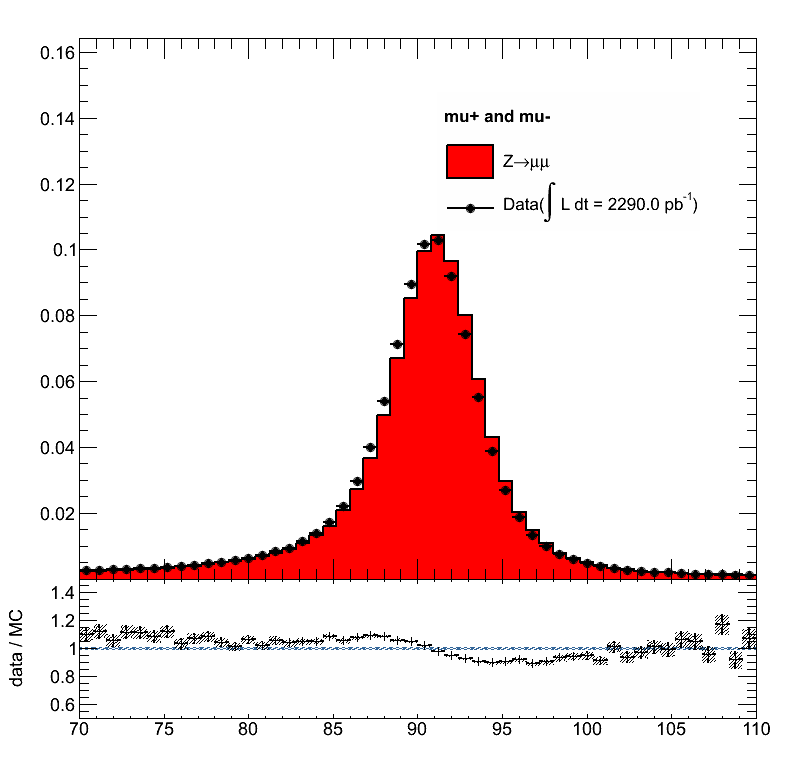
\includegraphics[width=0.44\textwidth]{perf/fig/KC_old}
        } 
        \subfigure[After scale corrections]{%
          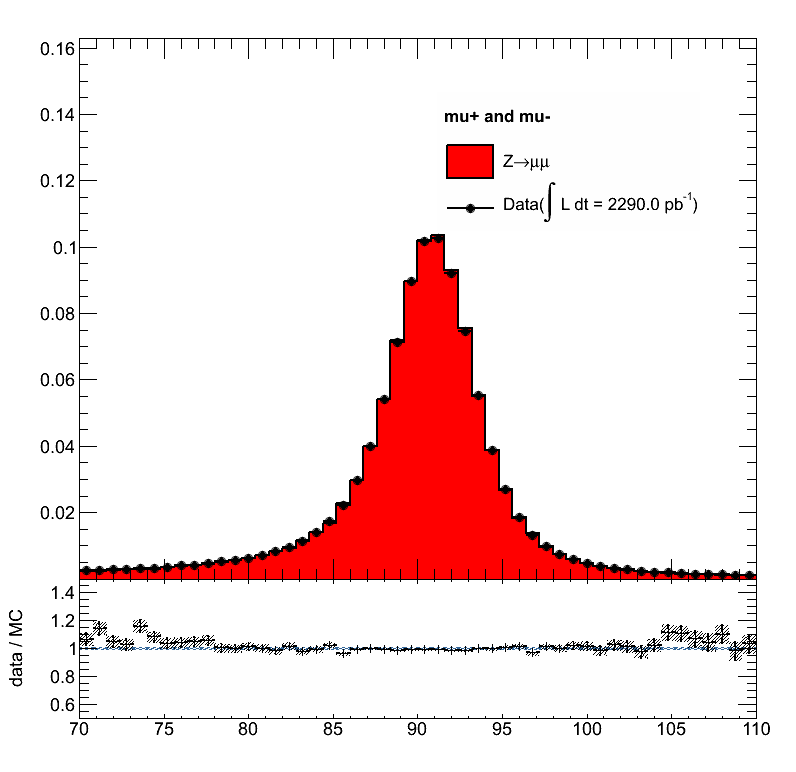
\includegraphics[width=0.44\textwidth]{perf/fig/KC_new}
        }
 \caption{ Effect of muon momentum scale corrections on the reconstructed \Zmm\ mass peak.}
 \label{fig:perf:mcpcorr}
 \end{center}
\end{figure}

\section{Missing Transverse Energy}
\label{perf:met:scale}
% https://cds.cern.ch/record/1548310/files/CERN-THESIS-2013-037.pdf
% https://indico.cern.ch/getFile.py/access?contribId=1&resId=0&materialId=slides&confId=161247

Missing transverse energy (\met) is used as a proxy for neutrino $p_T$ in \Wmn\ decays. Neutrinos interact with material so weakly that they always escape the detector, leaving an energy imbalance in the calorimeter. \met\ is defined as the transverse portion of this imbalance.

This analysis relies on the MET\_RefFinal algorithm to calculate \met~\cite{ATLAS-CONF-2012-101, Aad:2012re}. Calorimeter cells are first associated with the physics objects (muons, electrons, ...) and calibrated according to the object type, and then added vectorially. An additional adjustment is made for the muon momentum.

Because a calorimeter cell can be associated with multiple reconstructed objects, care must be taken to ensure that each cell contributes to \met\ calculation only once. This is accomplished by choosing the calibration for each cell in the following order of priority:
\begin{itemize}
\item MET\_RefEle - electrons
\item MET\_RefGamma - photons
\item MET\_RefTau - $\tau$ leptons that decayed hadronically
\item MET\_RefJet - jets with $p_T>20\ GeV$
\item MET\_RefMuon - energy deposited by muons in the calorimeter (usually a few GeV)
\item MET\_SoftJet - jets with $p_T<20\ GeV$
\item MET\_CellOutEflow - calorimeter cells not associated with any object
\end{itemize}

Additionally, a MET\_MuonBoy term, representing muon $p_T$, is added to the \met\ calculation because muons deposit only a small amount of their energy in the calorimeter

All analysis-level corrections to various event objects, such as corrections of the muon momentum or jet energy, are propagated to \met. The \MET\ uncertainty due to soft terms (cells that are not associated to any physics object) is evaluated by studying fake \MET\ in Z events and by comparing tracker and calorimeter measurements of electron momentum (E/p). The soft terms uncertainty is provided separately for \MET\ resolution and scale, and includes the effects of pileup on the calorimeters.

\subsection{Jet Reconstruction}
Although jets are not used explicitly in this analysis, they must be measured well to ensure a reliable estimation of missing transverse energy.

Jets are reconstructed from calorimeter topo-clusters (topologically connected groups of cells with energy deposition) using the anti-kT algorithm with cone size 0.4~\cite{Cacciari:2008gp}. They are subsequently calibrated using a four-step procedure illustrated in Fig.~\ref{fig:perf:jetcalib}. Further details are available in reference~\cite{ATLAS-CONF-2013-004}.

\begin{figure}[phtb]
  \begin{center}
    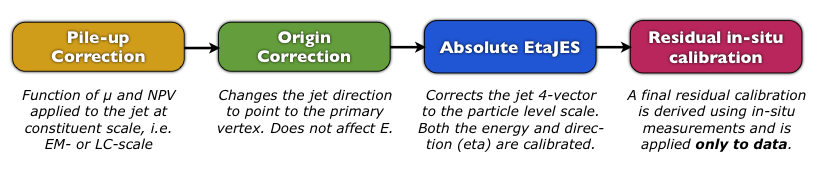
\includegraphics[width=0.99\textwidth]{perf/fig/calib}
 \caption{ An overview of the jet calibration scheme in ATLAS. A series of corrections are derived and applied to jet energy and direction.}
 \label{fig:perf:jetcalib}
 \end{center}
\end{figure}


%7
\chapter{Event Selection}
\label{chap:evt}
% event stuff

A series of selection cuts are applied to data and Monte-Carlo samples to obtain a high-purity sample of \Wboson\ event candidates. Following a summary table, this chapter explains the motivation behind some of the cuts, describes the selection efficiency in data and Monte-Carlo, and shows the kinematic distributions of selected events.

\section{Summary of Selection}
\label{sec:event:fullsel}

\begin{itemize}
\item Veto events not in the Good Run List (data only).
\item Reject events suffering from noise burst with \verb|larError| $> 1$.
\item Require the first reconstructed primary vertex in the collection to have $\ge 3$ associated tracks.
\item Events must be triggered by the single muon trigger.
\item Events are required to have one reconstructed muon, passing the following cuts:
  \begin{itemize}
  \item Combined STACO muon
  \item Track quality criteria
  \item $\abseta < 2.4$
  \item $\pt > 25\gev$ ($\pt > 20\gev$ for double-differential measurement)
  \item Track isolation
  \end{itemize}
\item Reject events with $> 1$ muon passing the above cuts.
\item The recommended \MET\ cleaning cuts are applied.
\item Veto events with a jet in a LAr hole.
\item $\met > 25\gev$.
\item $\mt = \sqrt{2 p_{T,\ell} \met \cdot (1 - \cos{\Delta\phi (\ell,
      \met) )}}> 40\gev$.
\end{itemize}

\subsection{Good Run List}
Events in luminosity blocks that suffered from severe detector defects (such as a non-operating calorimeter) are excluded from the very beginning. This cut is only applied in data because Monte-Carlo does not simulate these defects.

%https://twiki.cern.ch/twiki/bin/viewauth/AtlasProtected/LArCleaningAndObjectQuality
\subsection{LAr Error}
The liquid argon calorimeter suffers from rare noise bursts and data integrity problems during readout. These conditions may bias the \met\ estimation, so the affected events are flagged and removed from the data.
 
\subsection{Primary Vertex}
The primary vertex with the highest scalar sum-$p_T$ of the tracks pointing to the vertex is required to have at least 3 tracks to ensure that it is reconstructed correctly. Good knowledge of the primary vertex is necessary for muon and jet reconstruction algorithms.

\subsection{Trigger}
The event is required to satisfy the EF\_mu18 or EF\_mu18\_medium triggers, as described in Sec.~\ref{sec:event:trig}. The Muid family of trigger was chosen over the alternative MuGirl chains due to $\eta$-asymmetric problems in the MuGirl trigger (see Appendix~\ref{appendix:ac}).

\subsection{Track Quality Criteria}
\label{subsec:TrackQuality}
Inner detector tracks associated with combined muons are required to satisfy a series of hit-level requirements to ensure good quality of the helix parameters and reduce fakes:

\begin{itemize}
\item If hits in the inner pixel layer are geometrically expected, then the muon track must have at least 
one inner pixel layer hit;
\item $N_{PIX}+N_{DEAD-PIX} >$ 1, where $N_{PIX}$ is the number of pixel hits and $N_{DEAD-PIX}$
      is the number of crossed dead pixel sensors;
\item $N_{SCT}+N_{DEAD-SCT} \ge$ 6, where $N_{SCT}$ is the number of SCT hits and $N_{DEAD-SCT}$
      is the number of crossed dead SCT sensors;
\item $N_{DEAD-PIX}+N_{DEAD-SCT} <$ 2;
\item A successful TRT extension is required in the eta acceptance of the TRT. 
If $N_{TRT-HITS}$ denote the number of TRT hits on the muon track, $N_{TRT-OUTLIERS}$ the number of 
TRT outliers on the muon track (hits that are away from any nearby tracks, or those that failed to form a smooth trajectory with a nearby Pixel+SCT track), and $N_{TRT} = N_{TRT-HITS}+N_{TRT-OUTLIERS}$, then
\begin{itemize}
\item in the interval $|\eta| <$ 1.9: $N_{TRT} >$ 5 and $N_{TRT-OUTLIERS}$/$N_{TRT} <$ 0.9 are required;
\item in the interval $|\eta| >$ 1.9: if $N_{TRT} >$ 5 then $N_{TRT-OUTLIERS}$/$N_{TRT} <$ 0.9 is 
required; if $N_{TRT} \le$ 5, the muon is accepted regardless of the number of outliers.
\end{itemize}
\end{itemize}

In addition, the muon track must point to within 10 mm of the primary vertex ($|z_{\mu}-z_{PV}| <$ 10 mm) to suppress cosmic rays.

\subsection{Muon Isolation}
\label{subsec:MuonIsolation}
Muons produced in \Wmn\ decays are expected to be isolated from nearby tracks, in contrast to muons produced in heavy-flavor decays and in-flight decays of kaons. This difference is exploited through a relative tracking isolation cut: the $p_T$-sum of all tracks within a cone of $\Delta R = 0.4$ around the muon (excluding the muon itself) is divided by the muon $p_T$, resulting in a dimensionless quantity that peaks at 0 for well-isolated muons.
\begin{equation}
I_\mu = \frac{p_T^\mathrm{cone40}}{p_T^{\mu}} < 0.1
\end{equation}\label{eq:isolation}

The difference in the relative isolation distributions for heavy-flavor QCD Monte-Carlo and \Wmn\ Monte-Carlo is illustrated in Fig.~\ref{fig:event:isoplot}.

\begin{figure}[htb]
  \begin{center}
    \includegraphics[width=0.7\textwidth]{event/fig/TEST_ISOPLOT_NEG_lepton_ptiso40r}
    \caption{Relative isolation $p_T^{cone40}/{p_T}$ for the signal (\Wmn) and heavy-flavor QCD Monte-Carlo ($b\overline{b} \rightarrow \mu$). The distributions are normalized to the same area}
    \label{fig:event:isoplot}
  \end{center}
\end{figure}

\subsection{Second Muon Veto}
Events with additional muons are rejected to minimize the \Zmm\ background.

\subsection{\met\ Cleaning}
Events containing a jet pointing to misbehaving section of the calorimeter are vetoed to avoid biasing \met\ reconstruction.

\subsection{LAr Hole Veto}
In late April of 2011, 6 front-end boards of the liquid argon calorimeter failed, resulting in a well-defined acceptance hole. Events with jets pointing in the overall direction of the LAr hole are rejected to avoid biasing \met.

\subsection{\met\ and $m_T$ cuts}
Missing transverse energy and W transverse mass cuts consistent with a \Wmn\ decay are applied to reject background events and make the experimental measurement in a phase space similar to that used at the generator level (Sec.~\ref{method:fid:space}).

\section{Selected Events in Data and MC}

\subsection{Cutflows}

\paragraph{Data}

The numbers of candidate events after the different selection cuts are given in Table \ref{tab:Wmunu:cutflow_data_pt25}.

\paragraph{Simulation}

The numbers of selected events after the different selection cuts are given in Tables \ref{tab:Wmunu:cutflow_mc_POS_pt25} ($W^{+} \rightarrow \mu^{+} \nu$) and \ref{tab:Wmunu:cutflow_mc_NEG_pt25} ($W^{-} \rightarrow \mu^{-} \nu$), using the nominal signal Monte-Carlo and applying all re-weightings and scale-factors. These tables reflect the actual Monte-Carlo statistics - in other words, the numbers have not been scaled to the integrated luminosity in the data.

\begin{table}
\begin{center}
\input{Wmunu/figures/cutflow/data_pt25}
\caption{ Cutflow for \Wmn\ candidate events in data ($p_T~>~25~\GeV$). Data events that don't have at least one 8 \GeV muon (of any kind) were dropped at the ntuple creation stage.}
\label{tab:Wmunu:cutflow_data_pt25}
\end{center}
\end{table}


\begin{table}
\begin{center}
\input{Wmunu/figures/cutflow/mc_POS_pt25}
\caption{ Cutflow for $W^{+} \rightarrow \mu^{+} \nu$ events in the nominal Monte Carlo signal sample~(Powheg+Pythia). Pileup, vertex position, and $p_T^{W}$  weights are applied, but the counts are not scaled to the integrated luminosity in the data. The number of selected events after the application of efficiency scale factors is shown in the last row. Note that the Monte-Carlo events are not restricted to a fiducial region at truth level, so the reported efficiencies are a mixture of acceptance and reconstruction efficiency factors. }
\label{tab:Wmunu:cutflow_mc_POS_pt25}
\end{center}
\end{table}


\begin{table}
\begin{center}
\input{Wmunu/figures/cutflow/mc_NEG_pt25}
\caption{ Cutflow for $W^{-} \rightarrow \mu^{-} \nu$ events in the nominal Monte Carlo signal sample~(Powheg+Pythia). Pileup, vertex position, and $p_T^{W}$  weights are applied, but the counts are not scaled to the integrated luminosity in the data. The number of selected events after the application of efficiency scale factors is shown in the last row. Note that the Monte-Carlo events are not restricted to a fiducial region at truth level, so the reported efficiencies are a mixture of acceptance and reconstruction efficiency factors.}
\label{tab:Wmunu:cutflow_mc_NEG_pt25}
\end{center}
\end{table}

\subsection{Kinematic distributions}
Kinematic distributions of the selected \Wmn\ candidate events are shown in Figs.~\ref{fig:Wmunu:mu_angle25}, \ref{fig:Wmunu:mu_kine25} and~\ref{fig:Wmunu:mt_pt25}. The muon $p_{T}$ cut is set to 25 \GeV. The normalizations for QCD predictions are obtained from a template fit to the $E_T^{Miss}$ distribution in the inclusive $\eta - p_{T}$ region, repeated separately for each systematic variation. The fits are performed as described in Sec.~\ref{sec:wmnu:qcdbkg}. The final Monte-Carlo histograms are normalized to data. This is also done separately for each systematic in order to accentuate the differences in shapes introduced by the systematic variations, rather than differences in overall normalization, which are dominated by the cross-section and PDF uncertainties.

For all plotted distributions, Monte-Carlo predictions agree with the data within their uncertainty bands. The large systematic uncertainty in the tails of \MET\ (Fig.~\ref{fig:Wmunu:mu_kine25}), \Wboson\ $m_T$ and \Wboson\ $p_T$ (Fig.~\ref{fig:Wmunu:mt_pt25}) distributions are largely correlated and are driven by the use of alternative Monte-Carlo generators, as described in Sec.~\ref{sec:sys:theoryunc}.

% Selected control plots in slices of muon $p_{T}$ are available in Appendix~\ref{sec:Wmunu:AppendixControlPtBins}
\begin{figure}[phtb]
  \begin{center}
        \subfigure[$\eta$ : $\mu^+$]{%
          \includegraphics[width=0.45\textwidth]{Wmunu/figures/control_plots/inclusive25/P_stack_d3_eta_lpt_met_y_2__1_z_0__1_POS}
        } 
       \subfigure[$\eta$ : $\mu^-$]{%
         \includegraphics[width=0.45\textwidth]{Wmunu/figures/control_plots/inclusive25/P_stack_d3_eta_lpt_met_y_2__1_z_0__1_NEG}
        } \\
 \caption{ Distributions of the muon $\eta$ for selected \Wmunup~(left) and \Wmunum~(right) events. }
 \label{fig:Wmunu:mu_angle25}
 \end{center}
\end{figure}

\begin{figure}[phtb]
  \begin{center}
        \subfigure[$p_T$ : $\mu^+$]{%
          \includegraphics[width=0.45\textwidth]{Wmunu/figures/control_plots/inclusive25/P_stack_lpt_POS}
        } 
       \subfigure[$p_T$ : $\mu^-$]{%
         \includegraphics[width=0.45\textwidth]{Wmunu/figures/control_plots/inclusive25/P_stack_lpt_NEG}
        } \\
        \subfigure[$E_T^{Miss}$ : $W^{+}$]{%
          \includegraphics[width=0.45\textwidth]{Wmunu/figures/control_plots/inclusive25/P_stack_d3_abseta_lpt_met_x_0__1_y_2__1_POS}
        } 
       \subfigure[$E_T^{Miss}$ : $W^-$]{%
         \includegraphics[width=0.45\textwidth]{Wmunu/figures/control_plots/inclusive25/P_stack_d3_abseta_lpt_met_x_0__1_y_2__1_NEG}
        } \\
 \caption{ Distributions of the muon $p_{T}$ (top) and missing transverse energy (bottom) for selected \Wmunup~(left) and \Wmunum~(right) events ($p_{T}~>~25~\GeV$). The high-\MET\ region suffers from a large shape uncertainty due to the choice of signal Monte-Carlo,specifically the parton shower and hadronization model (see \Fig~\ref{fig:Wmunu:qcd_val_generators}). This shape uncertainty is included in the systematic band. }
 \label{fig:Wmunu:mu_kine25}
 \end{center}
\end{figure}


\begin{figure}[phtb]
  \begin{center}
        \subfigure[$m_T$ : $W^{+}$]{%
          \includegraphics[width=0.45\textwidth]{Wmunu/figures/control_plots/inclusive25/P_stack_d3_abseta_lpt_wmt_x_0__1_y_2__1_POS}
        } 
       \subfigure[$m_T$ : $W^-$]{%
         \includegraphics[width=0.45\textwidth]{Wmunu/figures/control_plots/inclusive25/P_stack_d3_abseta_lpt_wmt_x_0__1_y_2__1_NEG}
        } \\
        \subfigure[$p_T$ : $W^{+}$]{%
          \includegraphics[width=0.45\textwidth]{Wmunu/figures/control_plots/inclusive25/P_stack_d3_abseta_lpt_wpt_x_0__1_y_2__1_POS}
        } 
       \subfigure[$p_T$ : $W^-$]{%
         \includegraphics[width=0.45\textwidth]{Wmunu/figures/control_plots/inclusive25/P_stack_d3_abseta_lpt_wpt_x_0__1_y_2__1_NEG}
        } \\
 \caption{ Distributions of transverse mass (top) and reconstructed boson $p_T$ (bottom) for selected \Wmunup~(left) and \Wmunum~(right) events ($p_{T}~>~25~\GeV$)}
 \label{fig:Wmunu:mt_pt25}
 \end{center}
\end{figure}


\subsection{Purity and stability}
\label{sec:appmigrations}
The purity (fraction of reconstructed events generated in the same bin) 
and the stability (fraction of generated events reconstructed in the same bin), 
as defined in \ref{sec:puritystability}, provide a measurement of the migrations in and out of a given bin, due to resolution effects.
These quantities are then used to guide the choice of the unfolding method used for the single and double-differential measurements.
The two methods considered are the bin-by-bin and the iterative Bayesian unfolding. An iterative correction
is preferred when sizable bin migrations are present, to correct for biases due to possible differences between data and simulation
in the shape of the measured spectrum. The number of iterations is always a compromise between
the reduction of the bias and the increase in the statistical uncertainty, due to bin correlations introduced by multiple iterations.

The purity and the stability for the single-differential measurement as a function of $\eta$
are reported in \Fig~\ref{fig:Wmunu:PurityStability1D}. Very low migrations are observed between bins and therefore small differences
are expected between the two unfolding methods. The percent difference in the unfolded spectrum for different numbers
of iterations relative to the result obtained with bin-by-bin corrections is shown in \Fig~\ref{fig:Wmunu:unftest1D} (left), together
with the statistical uncertainty of the measurement in the different cases (right). As expected, negligible bin migrations lead to small differences between the two approaches. The bin-by-bin correction is therefore chosen for the final measurement of the single-differential cross-section.

\begin{figure}[phtb]
  \begin{center}
        \subfigure[Purity : \Wmunup]{%
          \includegraphics[width=0.45\textwidth]{Wmunu/figures/res/Wmn_PURITY_1D_PT25_POS_Purity_1d_proj}
        } 
       \subfigure[Purity : \Wmunum]{%
         \includegraphics[width=0.45\textwidth]{Wmunu/figures/res/Wmn_PURITY_1D_PT25_NEG_Purity_1d_proj}
        } \\
        \subfigure[Stability : \Wmunup]{%
          \includegraphics[width=0.45\textwidth]{Wmunu/figures/res/Wmn_STABIL_1D_PT25_POS_Stability_1d_proj}
        } 
       \subfigure[Stability : \Wmunum]{%
         \includegraphics[width=0.45\textwidth]{Wmunu/figures/res/Wmn_STABIL_1D_PT25_NEG_Stability_1d_proj}
        } \\
 \caption{Purity (top) and stability (bottom) for the single-differential binning for the \Wmunup~(left) and \Wmunum~(right) measurements.}
 \label{fig:Wmunu:PurityStability1D}
 \end{center}
\end{figure}

\begin{figure}[phtb]
  \begin{center}
        \subfigure[Percent deviations : \Wmunup]{%
          \includegraphics[width=0.45\textwidth]{Wmunu/figures/res/Wmn_UNFTST_1D_PT25_POS_unfIte_proj}
        } 
       \subfigure[Percent deviations : \Wmunum]{%
         \includegraphics[width=0.45\textwidth]{Wmunu/figures/res/Wmn_UNFTST_1D_PT25_NEG_unfIte_proj}
        } \\
        \subfigure[Statistical uncertainty : \Wmunup]{%
          \includegraphics[width=0.45\textwidth]{Wmunu/figures/res/Wmn_UNCTST_1D_PT25_POS_statUnfIte_proj}
        } 
       \subfigure[Statistical uncertainty : \Wmunum]{%
         \includegraphics[width=0.45\textwidth]{Wmunu/figures/res/Wmn_UNCTST_1D_PT25_NEG_statUnfIte_proj}
        } \\
    \caption{Percent deviation of the Bayesian-unfolded distribution for different numbers of iterations relative to the value obtained with bin-by-bin corrections (top) and statistical uncertainty for different unfolding options (bottom). These figures refer to the single-differential \Wmunup~(left) and \Wmunum~(right) cross-section measurements. For the percent-deviation plots, the Bayesian curves between 2 and 10 iterations appear on top of each other because the differences are smaller than the plotted marker size.}
 \label{fig:Wmunu:unftest1D}
 \end{center}
\end{figure}

The double-differential measurement in $\eta$ and $p_T$ bins is expected to suffer
from larger bin migrations due to the worse resolution on muon momentum and much steeper shape of the $p_T$
spectrum, as compared to pseudorapidity. The purity and stability in double-differential bins
are reported in \Fig~\ref{fig:Wmunu:PurityStability2D}. In some regions on the phase space, such as forward $\eta$ 
and moderate $p_T$, up to 35\% of events are reconstructed or generated in a wrong bin. Virtually all migrations
happen across $p_T$ (as opposed to $\eta$) bins. Therefore, the double-differential measurement is unfolded as a function
of $p_T$ inside each $\eta$ slice.

\begin{figure}[phtb]
  \begin{center}
        \subfigure[Purity : \Wmunup]{%
          \includegraphics[width=0.45\textwidth]{Wmunu/figures/purity/purity_2D_pos}
        } 
       \subfigure[Purity : \Wmunum]{%
         \includegraphics[width=0.45\textwidth]{Wmunu/figures/purity/purity_2D_neg}
        } \\
        \subfigure[Stability : \Wmunup]{%
          \includegraphics[width=0.45\textwidth]{Wmunu/figures/purity/stability_2D_pos}
        } 
       \subfigure[Stability : \Wmunum]{%
         \includegraphics[width=0.45\textwidth]{Wmunu/figures/purity/stability_2D_neg}
        } \\
 \caption{Purity (top) and stability (bottom) in percent for the double differential binning for the \Wmunup~(left) and \Wmunum~(right) measurements.}
 \label{fig:Wmunu:PurityStability2D}
 \end{center}
\end{figure}

Bin-by-bin and iterative Bayesian unfolding methods in the context of the double-differential measurement are compared in Fig.~\ref{fig:Wmunu:unftest_2D_POS}~-~\ref{fig:Wmunu:unctest_2D_NEG} for a few representative bins. The difference between these unfolding methods results in small uncertainties compared to other sources of systematic uncertainty. The more robust bin-by-bin correction is therefore chosen for the final measurement of the double-differential cross-section.

%% Unftest

\begin{figure}[phtb]
  \begin{center}
        \subfigure[\etaOne]{%
          \includegraphics[width=0.45\textwidth]{Wmunu/figures/res/Wmn_UNFTST_2D_PT20_POS_unfIte_2d_Slice_1_proj}
        } 
        \subfigure[\etaFive]{%
          \includegraphics[width=0.45\textwidth]{Wmunu/figures/res/Wmn_UNFTST_2D_PT20_POS_unfIte_2d_Slice_5_proj}
        } \\ 
       \subfigure[\etaEight]{%
         \includegraphics[width=0.45\textwidth]{Wmunu/figures/res/Wmn_UNFTST_2D_PT20_POS_unfIte_2d_Slice_9_proj}
       }
       \subfigure[\etaTenMu]{%
         \includegraphics[width=0.45\textwidth]{Wmunu/figures/res/Wmn_UNFTST_2D_PT20_POS_unfIte_2d_Slice_11_proj}
        } \\
    \caption{Percent deviations of the Bayesian-unfolded distributions for different numbers of iterations 
      relative to the value obtained with bin-by-bin corrections. These figures refer to the double-differential
      \Wmunup\ cross-section measurement unfolded as a function of muon $p_T$ inside four representative $\eta$ slices. }
 \label{fig:Wmunu:unftest_2D_POS}
 \end{center}
\end{figure}

\newpage
\begin{figure}[phtb]
  \begin{center}
        \subfigure[\etaOne]{%
          \includegraphics[width=0.45\textwidth]{Wmunu/figures/res/Wmn_UNFTST_2D_PT20_NEG_unfIte_2d_Slice_1_proj}
        } 
        \subfigure[\etaFive]{%
          \includegraphics[width=0.45\textwidth]{Wmunu/figures/res/Wmn_UNFTST_2D_PT20_NEG_unfIte_2d_Slice_5_proj}
        } \\ 
       \subfigure[\etaEight]{%
         \includegraphics[width=0.45\textwidth]{Wmunu/figures/res/Wmn_UNFTST_2D_PT20_NEG_unfIte_2d_Slice_9_proj}
       }
       \subfigure[\etaTenMu]{%
         \includegraphics[width=0.45\textwidth]{Wmunu/figures/res/Wmn_UNFTST_2D_PT20_NEG_unfIte_2d_Slice_11_proj}
        } \\
    \caption{Percent deviations of the Bayesian-unfolded distributions for different number of iterations 
      relative to the value obtained with bin-by-bin corrections. These figures refer to the double-differential
      \Wmunum\ cross-section measurement unfolded as a function of muon $p_T$ inside four representative $\eta$ slices. }
 \label{fig:Wmunu:unftest_2D_NEG}
 \end{center}
\end{figure}


%%%%%%%%%%%%%%%%%%%%%%%%%%%%%%%%%%%%
%% Unctest
%%%%%%%%%%%%%%%%%%%%%%%%%%%%%%%%%%%%

\newpage
\begin{figure}[phtb]
  \begin{center}
        \subfigure[\etaOne]{%
          \includegraphics[width=0.45\textwidth]{Wmunu/figures/res/Wmn_UNCTST_2D_PT20_POS_statUnfIte_2d_Slice_1_proj}
        } 
        \subfigure[\etaFive]{%
          \includegraphics[width=0.45\textwidth]{Wmunu/figures/res/Wmn_UNCTST_2D_PT20_POS_statUnfIte_2d_Slice_5_proj}
        } \\ 
       \subfigure[\etaEight]{%
         \includegraphics[width=0.45\textwidth]{Wmunu/figures/res/Wmn_UNCTST_2D_PT20_POS_statUnfIte_2d_Slice_9_proj}
       }
       \subfigure[\etaTenMu]{%
         \includegraphics[width=0.45\textwidth]{Wmunu/figures/res/Wmn_UNCTST_2D_PT20_POS_statUnfIte_2d_Slice_11_proj}
        } \\
    \caption{Statistical uncertainty for different unfolding options. These figures refer to the double-differential
      \Wmunup\ cross-section measurement unfolded as a function of muon $p_T$ inside four representative $\eta$ slices. }
 \label{fig:Wmunu:unctest_2D_POS}
 \end{center}
\end{figure}

\newpage
\begin{figure}[phtb]
  \begin{center}
        \subfigure[\etaOne]{%
          \includegraphics[width=0.45\textwidth]{Wmunu/figures/res/Wmn_UNCTST_2D_PT20_NEG_statUnfIte_2d_Slice_1_proj}
        } 
        \subfigure[\etaFive]{%
          \includegraphics[width=0.45\textwidth]{Wmunu/figures/res/Wmn_UNCTST_2D_PT20_NEG_statUnfIte_2d_Slice_5_proj}
        } \\ 
       \subfigure[\etaEight]{%
         \includegraphics[width=0.45\textwidth]{Wmunu/figures/res/Wmn_UNCTST_2D_PT20_NEG_statUnfIte_2d_Slice_9_proj}
       }
       \subfigure[\etaTenMu]{%
         \includegraphics[width=0.45\textwidth]{Wmunu/figures/res/Wmn_UNCTST_2D_PT20_NEG_statUnfIte_2d_Slice_11_proj}
        } \\
    \caption{Statistical uncertainty for different unfolding options. These figures refer to the double-differential
      \Wmunum\ cross-section measurement unfolded as a function of muon $p_T$ inside four representative $\eta$ slices. }
 \label{fig:Wmunu:unctest_2D_NEG}
 \end{center}
\end{figure}



%8
\chapter{Backgrounds}
\label{chap:bg}
% backgrounds

\section{Electroweak and Top Backgrounds}
\label{sec:Wmunu:EWKbackground}
Electroweak and top quark backgrounds are estimated using Monte Carlo. A systematic uncertainty is assigned by varying the normalizations according to the sample's cross section uncertainty. The normalizations of the W/Z, diboson, $t\bar{t}$ and single top are varied according to the cross-section Table~\ref{tab:samples}.

\section{QCD Background}
\label{sec:wmnu:qcdbkg}

The QCD background in the $W \rightarrow \mu \nu$ channel, also known as the multi-jet background, consists mainly of real muons produced in decays of heavy-flavor mesons.
The \MET\ distribution in such events is peaked at lower values than in real \Wmn\ events (Fig.~\ref{fig:Wmunu:qcd_met_shape_ewk}) and can be used as a discriminating variable in the QCD background determination.

\begin{figure}[phtb]
  \begin{center}
    \includegraphics[width=0.8\textwidth]{Wmunu/figures/met_shape/P_metshape_POS}
    \caption{Comparison of the shape of the \MET\ distribution between the signal + EWK + tops template and the QCD control sample for \Wmunup\ selection.}
    \label{fig:Wmunu:qcd_met_shape_ewk}
  \end{center}
\end{figure}

The QCD background is estimated using a partially data-driven technique. A two component binned maximum likelihood template fit using
Poisson statistics~\cite{Barlow:1993dm} is performed on \MET.

The signal + non-QCD background template is constructed from Monte-Carlo by applying the full signal selection, except the \MET\ cut. The
normalization of the various background components is obtained by
scaling the individual samples to a common luminosity using the cross
sections in Table~\ref{tab:samples}.
The relative normalization between the different Monte Carlo samples is then held fixed during the fit.
However, the normalization of the overall (signal + non-QCD) template is allowed to float to avoid biasing
the fit.

The template shape for the QCD background is obtained from data. The selection of this control sample follows the regular \Wmn\ selection, except for the following cuts, which are chosen in order to obtain a QCD-enriched and largely signal-free sample.

\begin{itemize}
\item The isolation requirement is dropped. Instead, one of the following isolation window requirements is applied:
\begin{itemize}
\item $p_T^{\mbox{cone20}} / p_T > 0.1$ and $p_T^{\mbox{cone20}} / p_T < 0.2$ (nominal)
\item $p_T^{\mbox{cone20}} / p_T > 0.12$ and $p_T^{\mbox{cone20}} / p_T < 0.25$ (systematic variation)
\item $p_T^{\mbox{cone40}} / p_T > 0.1$ and $p_T^{\mbox{cone40}} / p_T < 0.2$ (systematic variation)
\end{itemize}
\item The muon charge requirement is dropped to increase the statistics in the QCD template. The same QCD template is used for $W^+$ and $W^-$.
\end{itemize}

\Fig~\ref{fig:Wmunu:qcd_val_shape} validates the \MET\ shape in the QCD control region using the heavy-flavor Monte-Carlo. In \Fig~\ref{fig:Wmunu:qcd_val_shape}(a), the two charges are shown to have compatible shapes, justifying the summation of $\mu^{+}$ and $\mu^{-}$ templates in order to enhance available statistics. In \Fig~\ref{fig:Wmunu:qcd_val_shape}(b), the \MET\ shapes in the signal region and several anti-isolation regions are also shown to be compatible.

\begin{figure}[phtb]
  \begin{center}
        \subfigure[Charge dependence]{%
          \includegraphics[width=0.60\textwidth]{Wmunu/figures/met_shape/qcd_charge_MET_SHAPE}
        } 
        \subfigure[Choice of anti-isolation]{%
          \includegraphics[width=0.60\textwidth]{Wmunu/figures/met_shape/qcd_isolation_MET_SHAPE}
        }
 \caption{ Validation of \MET\ shapes in heavy-flavor Monte-Carlo:
 (a) events satisfying \Wmunup\ and \Wmunum\ selection
 (b) different anti-isolation windows.
 The transverse mass cut was relaxed to enhance the number of events available for comparison. }
 \label{fig:Wmunu:qcd_val_shape}
 \end{center}
\end{figure}

Electroweak and top contamination is subtracted from the QCD template using the nominal cross sections from table~\ref{tab:samples}.

The template fits are performed separately for $W^+$ and $W^-$, integrated over the entire fiducial volume, as well as for each $\eta$ and $\eta \times p_T$ bin of the single and double differential measurement respectively. The nominal fit range is chosen to between 0 and 60 GeV to avoid the high-\MET\ region that suffers from large shape differences depending on a choice of Monte-Carlo (see \Fig~\ref{fig:Wmunu:qcd_val_generators}). The bin size of the templates is motivated by the limited statistics in the QCD control sample and is chosen to be 2 GeV.

\begin{figure}[phtb]
  \begin{center}
        \subfigure[\Powheg\Pythia]{%
          \includegraphics[width=0.3\textwidth]{Wmunu/figures/met_shape/Q1_powheg_pythia}
        } 
        \subfigure[\Powheg\Herwig]{%
          \includegraphics[width=0.3\textwidth]{Wmunu/figures/met_shape/Q1_powheg_herwig}
        }
        \subfigure[\Mcatnlo]{%
          \includegraphics[width=0.3\textwidth]{Wmunu/figures/met_shape/Q1_mcnlo}
        }
 \caption{ Fitted \MET\ distributions for the three generators used in the analysis, showing different modeling of the high-\MET\ tail. }
 \label{fig:Wmunu:qcd_val_generators}
 \end{center}
\end{figure}

\subsection{Template Fits}
% The full set of fitted distributions in each bin in the single and double differential measurements can be found in the Appendix~\ref{sec:Wmunu:AppendixFitResults}. 
The fitted \MET\ distributions for the integrated measurement are shown in \Fig~\ref{fig:Wmunu:qcd_met_fits_int}.
\Fig~\ref{fig:Wmunu:qcd_met_fits_sample_bins} shows the fitted distributions for \Wmunup\ in four representative bins of $\eta$ and $p_T$. After the normalization for the QCD template is determined from the fit, a scale factor is computed as the ratio of the original and fitted integrals of the QCD template in the control region. This scale factor is used to properly scale the number of QCD background events in the signal region.

%%%%%%%%%%%%%%%%%%%%%%%%%%%%%%%%%%%%%%%%%%%%%%%%%%%%%%%%%%%%%%%%%%%%%%%%%%%%%%%%
%% Inclusive
%%%%%%%%%%%%%%%%%%%%%%%%%%%%%%%%%%%%%%%%%%%%%%%%%%%%%%%%%%%%%%%%%%%%%%%%%%%%%%%%

\begin{figure}[phtb]
  \begin{center}
        \subfigure[$W^+ \rightarrow \mu^+ \nu$]{%
          \includegraphics[width=0.4\textwidth]{Wmunu/figures/met_shape/Q0_powheg_pythia}
        } 
        \subfigure[$W^- \rightarrow \mu^- \nu$]{%
	  \includegraphics[width=0.4\textwidth]{Wmunu/figures/met_shape/Q1_powheg_pythia}
        }
	 \caption{Nominal QCD \MET\ fits for the integrated measurement for \Wmunup~(left) and \Wmunum~(right). Note that although \MET\ is plotted over a wider range, the fit only uses the bins between 0 and 60~\GeV. }
 \label{fig:Wmunu:qcd_met_fits_int}
 \end{center}
\end{figure}

%%%%%%%%%%%%%%%%%%%%%%%%%%%%%%%%%%%%%%%%%%%%%%%%%%%%%%%%%%%%%%%%%%%%%%%%%%%%%%%%
%% Representative
%%%%%%%%%%%%%%%%%%%%%%%%%%%%%%%%%%%%%%%%%%%%%%%%%%%%%%%%%%%%%%%%%%%%%%%%%%%%%%%%
\begin{figure}[phtb]
  \begin{center}
    \subfigure[$0.21 < |\eta| < 0.42$, \ptOne]{%
      \includegraphics[width=0.45\textwidth]{Wmunu/figures/qcdfits/Q0_x_2_2_y_2_2}
    } 
    \subfigure[$2.18 < |\eta| < 2.40$, \ptOne]{%
      \includegraphics[width=0.45\textwidth]{Wmunu/figures/qcdfits/Q0_x_11_11_y_2_2}
    } \\

    \subfigure[$0.21 < |\eta| < 0.42$, \ptFive]{%
      \includegraphics[width=0.45\textwidth]{Wmunu/figures/qcdfits/Q0_x_2_2_y_6_6}
    } 
    \subfigure[$2.18 < |\eta| < 2.40$, \ptFive]{%
      \includegraphics[width=0.45\textwidth]{Wmunu/figures/qcdfits/Q0_x_11_11_y_6_6}
    } \\

    \caption{Fitted \MET\ distributions for \Wmunup\ in four representative bins of $\eta$ and $p_T$. The dotted line indicates the upper limit of the fit range. The points in the fit range are allowed to shift independently within their uncertainties to achieve an arrangement that maximizes the TFractionFitter likelihood. These bin-by-bin adjustments are not shown in the plot, but are taken into account in the $\chi^2$ calculation. }
    \label{fig:Wmunu:qcd_met_fits_sample_bins}
  \end{center}
\end{figure}

\subsection{QCD Background Uncertainty}

In order to assign a systematic uncertainty to the QCD background, the fits are repeated for several variations, described below:

\begin{itemize}
\item Choice of signal template:
\begin{itemize}
\item The impact of the parton shower and hadronization model is tested by comparing the fit results using the nominal \Powheg\Pythia\ sample and a \Powheg\Herwig\ sample.
\item The uncertainty due to modeling of the hard-scattering matrix element is taken to be the difference of fit results obtained by using the \Powheg\Herwig\ and \Mcatnlo\ signal samples.
\end{itemize}
\item Choice of QCD template based on three anti-isolation windows, as described above.
\item Choice of the \MET\ fit range (5-50 GeV versus 0-60 GeV).
\item Choice of fit variable: \MET\ versus W transverse mass. The latter fit is performed in the 40-100 GeV range.
\item Systematic uncertainties on muon momentum, jet energy, and the soft \MET\ components are propagated to all Monte-Carlo \MET templates by varying the scale or resolution of the corresponding objects. The fits are repeated for each variation.
%% \item Electroweak templates were reweighed using the LHAPDF library to the following NLO PDFs (nominal samples use the CT10 PDF). The change in QCD background from PDF modeling is negligible.
%% \begin{verbatim}
%% - MSTW2008nlo68cl
%% - HERAPDF15NLO_EIG
%% - NNPDF23_nlo_as_0118
%% - abm11_5n_nlo
%% \end{verbatim}
\item Electroweak W and Z templates are reweighed to two alternative boson $p_T$ targets (\Sherpa\ and \Powheg\Pythiaeight)
\item Pileup uncertainty on electroweak templates is estimated by considering two variations:
\begin{itemize}
\item Scaling the number of interactions per bunch crossing in Monte-Carlo by an additional 3\%.
\item Splitting the fit into two parts: earlier, lower-pileup data (periods D-K) and later, higher-pileup data (L-M). Predicted QCD counts from the two fits are added and compared with the nominal, full-2011 fit (periods D-M).
\end{itemize}
\item Finally, a statistical uncertainty on the QCD template fraction, as reported by TFractionFitter, is treated as uncorrelated across bins and propagated through the master cross-section formula~\ref{eq:WZxsec}.
\end{itemize}

For example, the effect of \MET\ scale and resolution uncertainties on the shape of the QCD template is illustrated in Fig.~\ref{fig:Wmunu:qcd_met_shapes_pthard}.

\begin{figure}[phtb]
  \begin{center}
    \includegraphics[width=0.45\textwidth]{Wmunu/figures/met_shape/P_metsys_POS_scale}
    \includegraphics[width=0.45\textwidth]{Wmunu/figures/met_shape/P_metsys_POS_reso}
    \caption{Effect of \MET\ scale (left) and resolution (right) uncertainties on the shape of the \MET\ distribution in the signal Monte-Carlo for \Wmunup\ selection.}
    \label{fig:Wmunu:qcd_met_shapes_pthard}
  \end{center}
\end{figure}

\subsection{QCD Systematics}
\label{sec:bg:qcdsyst}

\begin{table}
  \footnotesize
  \begin{center}
  
    \begin{tabular}{lrr|rr}
      \hline
      \hline
       & \multicolumn{2}{c|}{$W^+ \rightarrow \mu^+ \nu$} & \multicolumn{2}{c}{$W^- \rightarrow \mu^- \nu$} \\
 Variation & $\delta N_{\mbox{QCD}} / N_{\mbox{QCD}}$ & $\delta N_{\mbox{QCD}} / N_{W+}^{\mbox{Cand.}}$ & $\delta N_{\mbox{QCD}} / N_{\mbox{QCD}}$ & $\delta N_{\mbox{QCD}} / N_{W^-}^{\mbox{Cand.}}$ \\
      \hline
    
Fit error  &  1.16\%  &  0.02\% & 	  1.00\%   &   0.03\% \\
Fit range  &  7.65\%  &  0.16\% & 	  5.51\%   &   0.18\% \\
Fit variable  &  12.27\%  &  0.26\% & 	  3.10\%   &   0.10\% \\
Period D-K and L-M fits  &  0.19\%  &  0.00\% & 	  0.17\%   &   0.01\% \\
Pileup scale 0.97  &  2.81\%  &  0.06\% & 	  1.53\%   &   0.05\% \\
MC parton shower  &  16.31\%  &  0.35\% & 	  4.46\%   &   0.15\% \\
MC matrix element  &  0.00\%  &  0.00\% & 	  0.00\%   &   0.00\% \\
$p_{T}^{W}$ reweighting  &  5.85\%  &  0.12\% & 	  4.89\%   &   0.16\% \\
EWK cross-section  &  0.68\%  &  0.01\% & 	  0.67\%   &   0.02\% \\
Top cross-section  &  0.00\%  &  0.00\% & 	  0.00\%   &   0.00\% \\
Type of anti-isolation  &  5.28\%  &  0.11\% & 	  5.26\%   &   0.17\% \\
MET soft scale  &  3.78\%  &  0.08\% & 	  2.54\%   &   0.08\% \\
MET soft resolution  &  3.29\%  &  0.07\% & 	  1.83\%   &   0.06\% \\
Muon momentum scale  &  1.72\%  &  0.04\% & 	  1.20\%   &   0.04\% \\
Muon momentum resolution  &  0.04\%  &  0.00\% & 	  0.14\%   &   0.00\% \\
Muon efficiencies  &  0.05\%  &  0.00\% & 	  0.10\%   &   0.00\% \\
Jet energy scale  &  1.66\%  &  0.04\% & 	  0.67\%   &   0.02\% \\
Jet energy resolution  &  3.31\%  &  0.07\% & 	  2.81\%   &   0.09\% \\
\hline	\hline
Total  &  24.26\%  &  0.51\% & 	  11.61\%   &   0.38\% \\

      \hline
      \hline
    \end{tabular}
    

    \caption{QCD uncertainties for the integrated \Wmunup\ and \Wmunum\ selections. Both the relative uncertainties on the QCD estimate, $\delta N_{QCD} / N_{QCD}$, and the absolute uncertainties divided by the total number of W events (selected W candidates in data after background subtraction) are shown. Some of the $W^+$ uncertainties are larger than their $W^-$ counterparts, possibly because the QCD background is smaller (as a percentage of the total background) in the $W^+$ selection, resulting in more volatility in the template fitter when it fits for small fractions. }
    \label{tab:Wmunu:qcd_unc_integrated}
  \end{center}
\end{table}

The systematic uncertainties assigned to the QCD estimate for the integrated $W^+$ and $W^-$ measurements are shown in \Tab~\ref{tab:Wmunu:qcd_unc_integrated}. \Fig~\ref{fig:Wmunu:qcd_unc_vsEta_pt25} shows the QCD uncertainties in bins of $\eta$ for the single-differential measurement with a $p_{T}$ cut of $25 \GeV$. Figures~\ref{fig:Wmunu:qcd_unc_vsEta_vsPt_pos_p1}~-~\ref{fig:Wmunu:qcd_unc_vsEta_vsPt_neg_p2} show the QCD uncertainties for a few representative bins in the the double-differential measurement.
Most components of the QCD uncertainty result in uncertainties on the cross section at or below the 0.2 \% level. However, the uncertainty assigned to the modeling of the signal sample, obtained by comparing the QCD estimates using \Powheg\Herwig\ and \Mcatnlo, has a larger contribution reaching 0.7\% in some of the $\eta$ bins. This uncertainty is dominated by the low statistics available in \Powheg\Herwig\ and \Mcatnlo\ signal samples, as evidenced by its large bin-by-bin fluctuations seen in \Fig~\ref{fig:Wmunu:qcd_unc_vsEta_pt25}.

The total uncertainty on the QCD estimate is obtained by adding all individual components in quadrature. The resulting uncertainty on the single-differential cross-section varies between 0.5\%~-~1.0\%. However, these numbers don't directly enter the final measured cross-sections because a majority of the systematic variations are in fact correlated with the corresponding variations in the \C\ factors (see Sec.~\ref{sec:xsec_formula}) and may interfere either constructively or destructively with them. Therefore, the systematic effects from the QCD background estimation are studied concurrently with the variations in the \C\ factors when applying the master cross-section formula~\ref{eq:WZxsec}.

\begin{figure}[phtb]
  \begin{center}
        \subfigure[QCD uncertainty / $N_{Expected}$: $W^+ \rightarrow \mu^+ \nu$]{%
          \includegraphics[width=0.60\textwidth]{Wmunu/figures/qcdunc/Q0_qcd_ptALL25_etaLOOP_syst_rel_bgsub}
        } 
       \subfigure[QCD uncertainty / $N_{Expected}$: $W^- \rightarrow \mu^- \nu$]{%
         \includegraphics[width=0.60\textwidth]{Wmunu/figures/qcdunc/Q1_qcd_ptALL25_etaLOOP_syst_rel_bgsub}
        } \\
 \caption{QCD uncertainties in per cent for the single-differential measurement in the \Wmunup\ (left) and \Wmunum\ (right) channels, $p_{T} > 25 \GeV$. The plot shows the absolute uncertainty in the number of QCD events divided by the number of W events (selected W candidates in data after background subtraction).}
 \label{fig:Wmunu:qcd_unc_vsEta_pt25}
 \end{center}
\end{figure}

\begin{figure}[phtb]
  \begin{center}
        \subfigure[\ptZero]{%
          \includegraphics[width=0.60\textwidth]{Wmunu/figures/qcdunc/Q0_qcd_pt1_etaLOOP_syst_rel_bgsub}
        } 
%        \subfigure[\ptOne]{%
%	  \includegraphics[width=0.60\textwidth]{Wmunu/figures/qcdunc/Q0_qcd_pt2_etaLOOP_syst_rel_bgsub}
%        } 
        \subfigure[\ptTwo]{%
	  \includegraphics[width=0.60\textwidth]{Wmunu/figures/qcdunc/Q0_qcd_pt3_etaLOOP_syst_rel_bgsub}
        }
 \caption{QCD uncertainties in per cent for the double-differential measurement in the \Wmunup\ channel in the lower-$p_{T}$ bins. Each plot shows the absolute uncertainty in the number of QCD events divided by the number of W events (selected W candidates in data after background subtraction).}
 \label{fig:Wmunu:qcd_unc_vsEta_vsPt_pos_p1}
 \end{center}
\end{figure}

\begin{figure}[phtb]
  \begin{center}
%        \subfigure[\ptThree]{%
%	  \includegraphics[width=0.60\textwidth]{Wmunu/figures/qcdunc/Q0_qcd_pt4_etaLOOP_syst_rel_bgsub}
%        } 
        \subfigure[\ptFour]{%
	  \includegraphics[width=0.60\textwidth]{Wmunu/figures/qcdunc/Q0_qcd_pt5_etaLOOP_syst_rel_bgsub}
        } 
%        \subfigure[\ptFive]{%
%	  \includegraphics[width=0.60\textwidth]{Wmunu/figures/qcdunc/Q0_qcd_pt6_etaLOOP_syst_rel_bgsub}
%        } 
        \subfigure[\ptSix]{%
	  \includegraphics[width=0.60\textwidth]{Wmunu/figures/qcdunc/Q0_qcd_pt7_etaLOOP_syst_rel_bgsub}
        } 
 \caption{QCD uncertainties in per cent for the double-differential measurement in the \Wmunup\ channel in the higher-$p_{T}$ bins. Each plot shows the absolute uncertainty in the number of QCD events divided by the number of W events (selected W candidates in data after background subtraction).}
 \label{fig:Wmunu:qcd_unc_vsEta_vsPt_pos_p2}
 \end{center}
\end{figure}

\begin{figure}[phtb]
  \begin{center}
        \subfigure[\ptZero]{%
          \includegraphics[width=0.60\textwidth]{Wmunu/figures/qcdunc/Q1_qcd_pt1_etaLOOP_syst_rel_bgsub}
        } 
%        \subfigure[\ptOne]{%
%	  \includegraphics[width=0.60\textwidth]{Wmunu/figures/qcdunc/Q1_qcd_pt2_etaLOOP_syst_rel_bgsub}
%        } 
        \subfigure[\ptTwo]{%
	  \includegraphics[width=0.60\textwidth]{Wmunu/figures/qcdunc/Q1_qcd_pt3_etaLOOP_syst_rel_bgsub}
        } 
 \caption{QCD uncertainties in per cent for the double-differential measurement in the \Wmunum\ channel in the lower-$p_T$ bins. Each plot shows the absolute uncertainty in the number of QCD events divided by the number of W events (selected W candidates in data after background subtraction).}
 \label{fig:Wmunu:qcd_unc_vsEta_vsPt_neg_p1}
 \end{center}
\end{figure}

\begin{figure}[phtb]
  \begin{center}
%        \subfigure[\ptThree]{%
%	  \includegraphics[width=0.60\textwidth]{Wmunu/figures/qcdunc/Q1_qcd_pt4_etaLOOP_syst_rel_bgsub}
%        } 
        \subfigure[\ptFour]{%
	  \includegraphics[width=0.60\textwidth]{Wmunu/figures/qcdunc/Q1_qcd_pt5_etaLOOP_syst_rel_bgsub}
        } 
%        \subfigure[\ptFive]{%
%	  \includegraphics[width=0.60\textwidth]{Wmunu/figures/qcdunc/Q1_qcd_pt6_etaLOOP_syst_rel_bgsub}
%        } 
        \subfigure[\ptSix]{%
	  \includegraphics[width=0.60\textwidth]{Wmunu/figures/qcdunc/Q1_qcd_pt7_etaLOOP_syst_rel_bgsub}
        } 
 \caption{QCD uncertainties in per cent for the double-differential measurement in the \Wmunum\ channel in the higher-$p_{T}$ bins. Each plot shows the absolute uncertainty in the number of QCD events divided by the number of W events (selected W candidates in data after background subtraction).}
 \label{fig:Wmunu:qcd_unc_vsEta_vsPt_neg_p2}
 \end{center}
\end{figure}


\section{Summary of Backgrounds}

The backgrounds to the \Wmn\ cross section measurements are small and well controlled. The QCD background, \Zmm, and $W \to \tau\nu$ are the most important backgrounds, followed by top pair production, $Z \to \tau\tau$ and dibosons. For the integrated measurement, QCD as well as the electroweak plus $t\bar{t}$ backgrounds are of the order $2-7\%$ as a percentage of data counts. A summary is given in \Tab~\ref{tab:WmunuAllbkg}.
The background composition for the single-differential and double-differential measurements are summarized in \Fig~\ref{fig:Wmunu:bg_frac_vsEta_pt25}~-~\ref{fig:Wmunu:BkgFractionsDoubleDiff_NEG}.

%% Integrated
\begin{table}
  \begin{center}
    \input{Wmunu/figures/bgcomp/bgcomp_ALL_pt25}
    \caption{ Background in \Wmn\ channels in per cent with statistical and systematic uncertainties given in that order. Integrated measurement, $p_T~>~25~\GeV$. }
    \label{tab:WmunuAllbkg}
  \end{center}
\end{table}

% bg summary plots
\begin{figure}[phtb]
  \begin{center}
        \subfigure[Backgrounds: $W^+ \rightarrow \mu^+ \nu$]{%
          \includegraphics[width=0.45\textwidth]{Wmunu/figures/bgcomp/bgsummary_POS_pt25}
        } 
       \subfigure[Backgrounds: $W^- \rightarrow \mu^- \nu$]{%
         \includegraphics[width=0.45\textwidth]{Wmunu/figures/bgcomp/bgsummary_NEG_pt25}
        } \\
    \caption{ Fractions of backgrounds as a percentage of data for the single-differential measurement in the \Wmunup\ (left) and \Wmunum\ (right) channels. The error bars correspond to the total (statistical  $\oplus$ systematic) uncertainties. For QCD background, the uncorrelated component of total uncertainty is shown separately as a solid band.}
 \label{fig:Wmunu:bg_frac_vsEta_pt25}
 \end{center}
\end{figure}

\clearpage
\begin{figure}[phtb]
  \begin{center}
        \subfigure[\ptZero]{%
	  \includegraphics[width=0.3\textwidth]{Wmunu/figures/bgcomp/bgsummary_POS_pt1}
        } 
        \subfigure[\ptOne]{%
	  \includegraphics[width=0.3\textwidth]{Wmunu/figures/bgcomp/bgsummary_POS_pt2}
        } \\
       \subfigure[\ptTwo]{%
	  \includegraphics[width=0.3\textwidth]{Wmunu/figures/bgcomp/bgsummary_POS_pt3}
        }
       \subfigure[\ptThree]{%
	  \includegraphics[width=0.3\textwidth]{Wmunu/figures/bgcomp/bgsummary_POS_pt4}
        }
       \subfigure[\ptFour]{%
	  \includegraphics[width=0.3\textwidth]{Wmunu/figures/bgcomp/bgsummary_POS_pt5}
        } \\
       \subfigure[\ptFive]{%
	  \includegraphics[width=0.3\textwidth]{Wmunu/figures/bgcomp/bgsummary_POS_pt6}
        }
       \subfigure[\ptSix]{%
	  \includegraphics[width=0.3\textwidth]{Wmunu/figures/bgcomp/bgsummary_POS_pt7}
       } 
      \caption{ Fractions of backgrounds as a percentage of data for the double-differential measurement with muon $p_{T} > 25 GeV$ (\Wmunup). The error bars correspond to the total (statistical  $\oplus$ systematic) uncertainties. For QCD background, the uncorrelated component of total uncertainty is shown separately as a solid band.}
    \label{fig:Wmunu:BkgFractionsDoubleDiff_POS}
 \end{center}
\end{figure}

\clearpage
\begin{figure}[phtb]
  \begin{center}
        \subfigure[\ptZero]{%
	  \includegraphics[width=0.3\textwidth]{Wmunu/figures/bgcomp/bgsummary_NEG_pt1}
        } 
        \subfigure[\ptOne]{%
	  \includegraphics[width=0.3\textwidth]{Wmunu/figures/bgcomp/bgsummary_NEG_pt2}
        } \\
       \subfigure[\ptTwo]{%
	  \includegraphics[width=0.3\textwidth]{Wmunu/figures/bgcomp/bgsummary_NEG_pt3}
        }
       \subfigure[\ptThree]{%
	  \includegraphics[width=0.3\textwidth]{Wmunu/figures/bgcomp/bgsummary_NEG_pt4}
        }
       \subfigure[\ptFour]{%
	  \includegraphics[width=0.3\textwidth]{Wmunu/figures/bgcomp/bgsummary_NEG_pt5}
        } \\
       \subfigure[\ptFive]{%
	  \includegraphics[width=0.3\textwidth]{Wmunu/figures/bgcomp/bgsummary_NEG_pt6}
        }
       \subfigure[\ptSix]{%
	  \includegraphics[width=0.3\textwidth]{Wmunu/figures/bgcomp/bgsummary_NEG_pt7}
       } 
    \caption{ Fractions of backgrounds as a percentage of data for the double-differential measurement with muon $p_{T} > 25 GeV$ (\Wmunum). The error bars correspond to the total (statistical  $\oplus$ systematic) uncertainties. For QCD background, the uncorrelated component of total uncertainty is shown separately as a solid band.}
    \label{fig:Wmunu:BkgFractionsDoubleDiff_NEG}
 \end{center}
\end{figure}


\clearpage

%9
\chapter{Uncertainties}
\label{chap:unc}
% systematics

\section{Statistical Uncertainties}
Statistical uncertainties arise from three sources:
\begin{itemize}
\item Limited amount of data in the analyzed sample
\item Limited number of simulated background events
\item Limited number of simulated \Wmn\ signal events.
\end{itemize}

All three sources of statistical uncertainty are propagated to the final measurement using the toy Monte-Carlo method with 200 iterations. For example, in the case of background statistics, the cross-section is re-calculated 200 times, each time taking the number of background events from a Gaussian centered at the nominal value $B$ and having its width set to $\delta B$. In the end, the RMS (root-mean-square) of 200 cross-section measurements is computed and taken as the statistical uncertainty. A similar procedure is repeated with variations in the number of data counts and in the efficiency factor \C\ derived from the signal Monte-Carlo.

\section{Systematic Uncertainties}

Uncertainties in reconstruction performance, simulation parameters, and detector conditions directly affect the value of the measured cross-section. The entire analysis chain was repeated under each systematic variation to assess the importance of these effects. The final uncertainty on the cross-section is formed as the sum-in-quadrature of the following individual components:

\begin{itemize}
\item Muon trigger efficiency.
\item Muon reconstruction efficiency:
\begin{itemize}
\item $p_T$ parametrization uncertainty,
\item Choice of probe (ID-only vs CaloTag muon).
\end{itemize}
\item Muon isolation efficiency.
\item Muon momentum resolution:
\begin{itemize}
\item Inner Detector (ID) part,
\item Muon Spectrometer (MS) part.
\end{itemize}
\item Muon momentum scale:
\begin{itemize}
\item Multiplicative scale,
\item Charge-splitting curvature correction.
\end{itemize}
\item $E_{T}^{miss}$ (soft terms):
\begin{itemize}
\item  $E_{T}^{miss}$ scale,
\item $E_{T}^{miss}$ resolution.
\end{itemize}
\item Jet energy:
\begin{itemize}
\item Jet energy scale,
\item Jet energy resolution.
\end{itemize}
\item Theoretical uncertainties:
\begin{itemize}
\item Matrix element (ME),
\item Parton shower (PS) and hadronization,
\item Parton Distribution Functions (PDF).
\end{itemize}
\item $p^{W}_{T}$ reweighting.
\item Pile-up uncertainty.
\item Background uncertainties:
\begin{itemize}
\item Electroweak and top backgrounds,
\item Multi-jet (QCD) background.
\end{itemize}
\end{itemize}

\subsection{Trigger, Reconstruction and Isolation Efficiencies}
Differences in the efficiencies measured in data and in Monte-Carlo are corrected using tag-and-probe scale factors, as described in Sec.~\ref{sec:perf:muoncorr}. These scale factors have two kinds of uncertainties: the truly systematic effects due to variations in the tag-and-probe procedure, and a statistical component due to limited Z-boson statistics available in the data.

The systematic variations are handled by re-calculating the cross-section under corresponding variations in the scale factors.

The statistical component is instead derived using the toy-MC method. 1000 replicas of the scale-factors are formed assuming a Gaussian distribution around the central values of these scale factors, with the width equal to their statistical uncertainty. The choice of such a large number of replicas is motivated by the desire to properly correlate the muon scale factor uncertainties between the \Wmn\ and \Zmm\ channels. These toys are propagated through the master cross-section formula~\ref{eq:WZxsec} to obtain a set of 1000 cross-section measurements, and the RMS is taken as the scale factor systematic.

\subsection{Muon Momentum}
Uncertainties related to the muon momentum measurement affect the \C\ factors that translate the measured event counts to a detector-invariant cross-section at the generator level. They can also produce migrations of events across $p_{T}$ bins.

Muons in the Monte Carlo are smeared to account for the extra momentum resolution as measured from data, as described in Sec.~\ref{perf:muon:scale}. Four systematic variations of the smearing parameters are available, corresponding to the up-down variations of the Inner Detector and Muon Spectrometer smearing constants.

Corrections to the transverse momentum of the muons are applied in Monte-Carlo events to improve their agreement with the data, as described in Sec.~\ref{perf:muon:scale}. Four systematic variations are applied, corresponding to the up-down variations for the overall momentum scale and for the charge-splitting curvature.

\subsection{\MET\ Scale and Resolution}
The effects on the \MET\ reconstruction due to the muon and jet energy scale and resolution uncertainties are taken into account by recalculating the \MET\ using the correspondingly shifted muon or jet objects. The effects on the \MET\ due to these variations are therefore implicitly included in the uncertainties quoted for muon/jet energy scale and resolution uncertainties. The \MET\ uncertainty due to ``soft'' clusters unassociated to any physics object is evaluated separately, as described in Sec.~\ref{perf:met:scale}. This uncertainty is propagated to the measurement by applying the up and down variations to the \MET\ scale and resolution in Monte-Carlo and evaluating the deviation of the resulting cross-section from the nominal value.

\subsection{Pile-Up}
Pile-up uncertainties are implicitly included in the uncertainties on the efficiency scale factors and \met scale and resolution. As an additional uncertainty, the number of interactions per bunch crossing is rescaled in Monte-Carlo by an additional 3\%.

\subsection{Boson $p_T$}
The uncertainty due to W $p_T$ reweighting (Sec.~\ref{sec:bosonptreweight}) is evaluated by reweighting the nominal Monte Carlo sample to a different boson $p_T$ target and taking the resulting deviation in the cross-section from the nominal value as an uncertainty. The alternative reweighting targets are based on PowhegPythia8 and Sherpa14 generators.

\subsection{Backgrounds}
The determination of background uncertainties was described in Chap.~\ref{chap:bg}.

Many of the systematic variations also affect the shape of the \met\ distribution in Monte-Carlo, which is used to fit for QCD fractions (Sec.~\ref{sec:wmnu:qcdbkg}). The resulting variations in QCD normalization are correlated with the corresponding variations of the electroweak backgrounds and the \C\ factors (Sec.~\ref{sec:xsec_formula}), and are thus included as part of those uncertainties. However, some variations are intrinsic to the fit procedure and are accounted for separately as a genuine ``QCD uncertainty''. Included among these are the choice of the QCD control region and the fit parameters, and the statistical fit uncertainty reported by the fraction fitter.

\subsection{Theoretical uncertainties}
\label{sec:sys:theoryunc}
Theoretical uncertainties are minimized by applying a similar kinematic selection at the truth and detector levels.

\paragraph{PDF}
PDF uncertainty is evaluated by separately calculating the \C\ factors and applying the master cross-section formula~\ref{eq:WZxsec} for each of the 52 error sets in the CT10 family. The resulting deviations are combined using the Hessian approach, as described in \cite{Lai:2010nw}, and rescaled from the 90\% to 68\% confidence interval.

\paragraph{Matrix Element}
The sensitivity of the \C\ factors (Sec.~\ref{sec:xsec_formula}) on the modeling of the hard-scatter process is evaluated by re-deriving them using the MC@NLO generator. The difference between the cross-sections derived with the MC@NLO and Powheg+Herwig \C\ factors is assigned as an uncertainty, which is treated as independent from the parton shower uncertainty described below.

\paragraph{Parton Shower}
The sensitivity of the \C\ factors (Sec.~\ref{sec:xsec_formula}) to the choice of the parton shower and hadronization model is evaluated by re-deriving the \C\ factors using the Powheg+Herwig generator instead of the nominal Powheg+Pythia generator, and assigning the deviation in the resulting cross-sections as an uncertainty.

\paragraph{Smoothing of Theory Systematics}
\label{sys:smoothing}
The systematic uncertainties assigned to the choice of the matrix-element generator (ME) and parton showering (PS) programs suffer from statistical fluctuations, due to the limited statistics of the alternative Monte Carlo samples (Powheg+Herwig and MC@NLO). This is especially problematic in the double-differential measurements, where statistical fluctuations cause substantial bin-to-bin variations in the assigned theoretical uncertainty. In order to overcome these unphysical fluctuations, the uncertainties due to the choice of the generator and parton showering programs are smoothed by performing a polynomial fit over the $\eta$ bins in each $p_T$ slice. Polynomials of 0th, 1st and 2nd order are considered. The choice of the signal Monte Carlo sample affects both the QCD estimation as well as the \C\ factors (Sec.~\ref{sec:xsec_formula}). The fits to the deviations of the cross-section due to variations of the signal sample used in the QCD estimation are shown in \Fig~\ref{fig:Wmunu:syst_smoothing_bkg}. \Fig~\ref{fig:Wmunu:syst_smoothing_unfolding} shows the corresponding plots for variations in the signal sample used to derive the \C\ factors.
% The fitted uncertainties for the case when both variations are done in parallel are shown in \Fig~\ref{fig:Wmunu:syst_smoothing_total}.

Similar plots for the double-differential measurement in $p_T$ bins are shown in Appendix~\ref{appendix:smoothing}.

Based on these plots, the 2nd order polynomial is chosen to smoothen the theory systematics. The fits to the deviations in the backgrounds and the \C\ factors are done independently, and the resulting systematic uncertainties are summed linearly. The uncertainty band around the fitted curves is used as an additional, bin-by-bin uncorrelated source of uncertainty.

\begin{figure}[phtb]
  \begin{center}
        \subfigure[$W^+$: Powheg+Herwig vs Powheg+Pythia]{%
          \includegraphics[width=0.45\textwidth]{Wmunu/figures/smoothing/1D_pt25_POS_PSsyst_onlybg}
        } 
       \subfigure[$W^-$ Powheg+Herwig vs Powheg+Pythia]{%
         \includegraphics[width=0.45\textwidth]{Wmunu/figures/smoothing/1D_pt25_NEG_PSsyst_onlybg}
        } \\
        \subfigure[$W^+$: MC@NLO vs Powheg+Herwig]{%
          \includegraphics[width=0.45\textwidth]{Wmunu/figures/smoothing/1D_pt25_POS_MEsyst_onlybg}
        } 
       \subfigure[$W^-$ MC@NLO vs Powheg+Herwig]{%
         \includegraphics[width=0.45\textwidth]{Wmunu/figures/smoothing/1D_pt25_NEG_MEsyst_onlybg}
        } \\
 \caption{Fits to the fractional deviation of the cross-section due to variations in the signal Monte Carlo sample used in the QCD fit. 
   The signal sample used to compute the \C\ factors is always Powheg+Pythia. Because it is difficult to correctly define the uncertainty from the QCD fit in each bin, the fit was performed disregarding the errors.}
 \label{fig:Wmunu:syst_smoothing_bkg}
 \end{center}
\end{figure}


\begin{figure}[phtb]
  \begin{center}
        \subfigure[$W^+$: Powheg+Herwig vs Powheg+Pythia]{%
          \includegraphics[width=0.45\textwidth]{Wmunu/figures/smoothing/1D_pt25_POS_PSsyst_onlyunf}
        } 
       \subfigure[$W^-$ Powheg+Herwig vs Powheg+Pythia]{%
         \includegraphics[width=0.45\textwidth]{Wmunu/figures/smoothing/1D_pt25_NEG_PSsyst_onlyunf}
        } \\
        \subfigure[$W^+$: MC@NLO vs Powheg+Herwig]{%
          \includegraphics[width=0.45\textwidth]{Wmunu/figures/smoothing/1D_pt25_POS_MEsyst_onlyunf}
        } 
       \subfigure[$W^-$ MC@NLO vs Powheg+Herwig]{%
         \includegraphics[width=0.45\textwidth]{Wmunu/figures/smoothing/1D_pt25_NEG_MEsyst_onlyunf}
        } \\
 \caption{Fits to the fractional deviation of the cross-section due to variations in the signal Monte Carlo sample used to compute the \C\ factors. 
 The signal sample used in the QCD fit is always Powheg+Pythia.}
 \label{fig:Wmunu:syst_smoothing_unfolding}
 \end{center}
\end{figure}

%% \begin{figure}[phtb]
%%   \begin{center}
%%         \subfigure[$W^+$: Powheg+Herwig vs Powheg+Pythia]{%
%%           \includegraphics[width=0.45\textwidth]{Wmunu/figures/smoothing/1D_pt25_POS_PSsyst_all}
%%         } 
%%        \subfigure[$W^-$ Powheg+Herwig vs Powheg+Pythia]{%
%%          \includegraphics[width=0.45\textwidth]{Wmunu/figures/smoothing/1D_pt25_NEG_PSsyst_all}
%%         } \\
%%         \subfigure[$W^+$: MC@NLO vs Powheg+Herwig]{%
%%           \includegraphics[width=0.45\textwidth]{Wmunu/figures/smoothing/1D_pt25_POS_MEsyst_all}
%%         } 
%%        \subfigure[$W^-$ MC@NLO vs Powheg+Herwig]{%
%%          \includegraphics[width=0.45\textwidth]{Wmunu/figures/smoothing/1D_pt25_NEG_MEsyst_all}
%%         } \\
%%  \caption{Fits to the fractional deviation of the cross-section due to variations in the signal Monte Carlo sample used both for the QCD estimate and the \C\ factors. The statistical uncertainty and systematic fluctuations on the fitted QCD fraction are not accounted for in the error bars. As a consequence, the error bars are under-estimated and the $\chi^2$ is over-estimated.}
%%  \label{fig:Wmunu:syst_smoothing_total}
%%  \end{center}
%% \end{figure}


\section{Luminosity Uncertainty}
The uncertainty on the integrated luminosity is 1.8\% (Sec.~\ref{mc:sec:coldata}) and is quoted separately from the other systematics. The main reason for its special treatment is because the luminosity uncertainty does not change the shape of any differential cross-section distributions, but only produces an overall shift. Therefore, it does not affect the fits to parton distribution functions, which typically probe the shape of the cross-section as a function of $\eta$.

\section{Summary of systematics}

The relative uncertainties, in percent, on the fiducial integrated measurement are summarized in Table \ref{tab:Wmunu:unfolded_unc_0d_pt25}. The relative uncertainties, in percent, on the fiducial single-differential and double-differential measurements are summarized in Fig.~\ref{fig:Wmunu:unfolded_unc_1d_pt25} and Figs.~\ref{fig:Wmunu:unfolded_unc_2d_1}~-~\ref{fig:Wmunu:unfolded_unc_2d_7}, respectively.

The systematic uncertainty on the fiducial integrated measurement is around 0.6\% for both charges, while the statistical uncertainty is only about 0.04\%. The dominant systematics come from QCD and electroweak backgrounds, followed by the theory uncertainties, muon reconstruction efficiency, W $p_T$ reweighting, and scale uncertainties on jets, muons, and \MET.\footnote{ Although the theory uncertainties (Parton Shower and Matrix Element) dominate the estimate of the QCD background (Sec.~\ref{sec:bg:qcdsyst}), their effect on the cross-section is largely compensated by the corresponding variations in the \C\ factors.} The measurement is clearly dominated by its systematics, in contrast to the 2010 result where statistical and systematic uncertainties were comparable in size. However, luminosity remains the dominant effect by far, resulting in an additional 1.8\% uncertainty. 

Systematic uncertainties on the single-differential measurement range between 0.6\%-1.0\% depending on $\eta$, while the statistical uncertainty is about 0.15\%. Similarly to the integrated measurement, QCD and electroweak backgrounds dominate the uncertainty.

Systematic uncertainties on the double-differential measurement are highly dependent on $p_T$. In the lowest $p_T$ bin (\ptZero), systematic uncertainty ranges between 7\%-13\% and is dominated by \MET\ resolution. The uncertainty drops to about 3\% in the \ptOne\ bin, lingers around 1\%-2\% for bins within $30<p_T<45$ GeV, and returns to 3\% for \ptFive. In these ranges of $p_T$, the uncertainty is dominated by theory (parton shower and matrix element). In the last bin, \ptSix, the systematic uncertainty reaches 4\% and is dominated by jet energy scale and resolution, since very high-$p_T$ muons usually balance against energetic jets.

\begin{table}
  \small
  \begin{center}
  \input{Wmunu/figures/res/Wmn_SYSTEM_0D_PT25_SUM_Unc_proj}
    \caption{Summary of the systematic uncertainties on the integrated  \Wmunum\ and \Wmunup\ cross-sections.}
    \label{tab:Wmunu:unfolded_unc_0d_pt25}
  \end{center}
\end{table}

\begin{figure}[phtb]
  \begin{center}
        \subfigure[\Wminus]{%
	  \includegraphics[width=0.60\textwidth]{Wmunu/figures/res/Wmn_SYSTEM_1D_PT25_NEG_Unc_proj}
        } \\
        \subfigure[\Wplus]{%
	  \includegraphics[width=0.60\textwidth]{Wmunu/figures/res/Wmn_SYSTEM_1D_PT25_POS_Unc_proj}
        }
 \caption{ Uncertainty on the single-differential \Wmunum\ (top) and \Wmunup\ (bottom) cross-sections. }
 \label{fig:Wmunu:unfolded_unc_1d_pt25}
 \end{center}
\end{figure}

%% \begin{figure}[phtb]
%%   \begin{center}
%%         \subfigure[\ptOne]{%
%% 	  \includegraphics[width=0.4\textwidth]{Wmunu/figures/res/Wmn_SYSTEM_2D_PT20_POS_Unc_2d_Slice_2.pdf}
%%         }
%%        \subfigure[\ptTwo]{%
%% 	  \includegraphics[width=0.4\textwidth]{Wmunu/figures/res/Wmn_SYSTEM_2D_PT20_POS_Unc_2d_Slice_3.pdf}
%%         } \\
%%        \subfigure[\ptThree]{%
%% 	  \includegraphics[width=0.4\textwidth]{Wmunu/figures/res/Wmn_SYSTEM_2D_PT20_POS_Unc_2d_Slice_4.pdf}
%%         }
%%        \subfigure[\ptFour]{%
%% 	  \includegraphics[width=0.4\textwidth]{Wmunu/figures/res/Wmn_SYSTEM_2D_PT20_POS_Unc_2d_Slice_5.pdf}
%%         } \\
%%        \subfigure[\ptFive]{%
%% 	  \includegraphics[width=0.4\textwidth]{Wmunu/figures/res/Wmn_SYSTEM_2D_PT20_POS_Unc_2d_Slice_6.pdf}
%%         }
%%        \subfigure[\ptSix]{%
%% 	  \includegraphics[width=0.4\textwidth]{Wmunu/figures/res/Wmn_SYSTEM_2D_PT20_POS_Unc_2d_Slice_7.pdf}
%%        } 
%%  \caption{ Uncertainty on the double-differential \Wmunup\ cross-section }
%%  \label{fig:Wmunu:unfolded_unc_2d_pos}
%%  \end{center}
%% \end{figure}

%% \begin{figure}[phtb]
%%   \begin{center}
%%         \subfigure[\ptOne]{%
%% 	  \includegraphics[width=0.4\textwidth]{Wmunu/figures/res/Wmn_SYSTEM_2D_PT20_NEG_Unc_2d_Slice_2.pdf}
%%         }
%%        \subfigure[\ptTwo]{%
%% 	  \includegraphics[width=0.4\textwidth]{Wmunu/figures/res/Wmn_SYSTEM_2D_PT20_NEG_Unc_2d_Slice_3.pdf}
%%         } \\
%%        \subfigure[\ptThree]{%
%% 	  \includegraphics[width=0.4\textwidth]{Wmunu/figures/res/Wmn_SYSTEM_2D_PT20_NEG_Unc_2d_Slice_4.pdf}
%%         }
%%        \subfigure[\ptFour]{%
%% 	  \includegraphics[width=0.4\textwidth]{Wmunu/figures/res/Wmn_SYSTEM_2D_PT20_NEG_Unc_2d_Slice_5.pdf}
%%         } \\
%%        \subfigure[\ptFive]{%
%% 	  \includegraphics[width=0.4\textwidth]{Wmunu/figures/res/Wmn_SYSTEM_2D_PT20_NEG_Unc_2d_Slice_6.pdf}
%%         }
%%        \subfigure[\ptSix]{%
%% 	  \includegraphics[width=0.4\textwidth]{Wmunu/figures/res/Wmn_SYSTEM_2D_PT20_NEG_Unc_2d_Slice_7.pdf}
%%        } 
%%  \caption{ Uncertainty on the double-differential \Wmunum\ cross-section }
%%  \label{fig:Wmunu:unfolded_unc_2d_neg}
%%  \end{center}
%% \end{figure}

\begin{figure}[phtb]
  \begin{center}
        \subfigure[\Wmunup]{%
	  \includegraphics[width=0.60\textwidth]{Wmunu/figures/res/Wmn_SYSTEM30_2D_PT20_POS_Unc_2d_Slice_1.pdf}
        } 
        \subfigure[\Wmunum]{%
	  \includegraphics[width=0.60\textwidth]{Wmunu/figures/res/Wmn_SYSTEM30_2D_PT20_NEG_Unc_2d_Slice_1.pdf}
        } 
 \caption{ Uncertainty on the double-differential \Wmn\ cross-section (\ptZero\ bin).}
 \label{fig:Wmunu:unfolded_unc_2d_1}
 \end{center}
\end{figure}

\begin{figure}[phtb]
  \begin{center}
        \subfigure[\Wmunup]{%
	  \includegraphics[width=0.60\textwidth]{Wmunu/figures/res/Wmn_SYSTEM_2D_PT20_POS_Unc_2d_Slice_2.pdf}
        } 
        \subfigure[\Wmunum]{%
	  \includegraphics[width=0.60\textwidth]{Wmunu/figures/res/Wmn_SYSTEM_2D_PT20_NEG_Unc_2d_Slice_2.pdf}
        } 
 \caption{ Uncertainty on the double-differential \Wmn\ cross-section (\ptOne\ bin).}
 \label{fig:Wmunu:unfolded_unc_2d_2}
 \end{center}
\end{figure}

\begin{figure}[phtb]
  \begin{center}
        \subfigure[\Wmunup]{%
	  \includegraphics[width=0.60\textwidth]{Wmunu/figures/res/Wmn_SYSTEM_2D_PT20_POS_Unc_2d_Slice_3.pdf}
        } 
        \subfigure[\Wmunum]{%
	  \includegraphics[width=0.60\textwidth]{Wmunu/figures/res/Wmn_SYSTEM_2D_PT20_NEG_Unc_2d_Slice_3.pdf}
        } 
 \caption{ Uncertainty on the double-differential \Wmn\ cross-section (\ptTwo\ bin).}
 \label{fig:Wmunu:unfolded_unc_2d_3}
 \end{center}
\end{figure}

\begin{figure}[phtb]
  \begin{center}
        \subfigure[\Wmunup]{%
	  \includegraphics[width=0.60\textwidth]{Wmunu/figures/res/Wmn_SYSTEM_2D_PT20_POS_Unc_2d_Slice_4.pdf}
        } 
        \subfigure[\Wmunum]{%
	  \includegraphics[width=0.60\textwidth]{Wmunu/figures/res/Wmn_SYSTEM_2D_PT20_NEG_Unc_2d_Slice_4.pdf}
        } 
 \caption{ Uncertainty on the double-differential \Wmn\ cross-section (\ptThree\ bin).}
 \label{fig:Wmunu:unfolded_unc_2d_4}
 \end{center}
\end{figure}

\begin{figure}[phtb]
  \begin{center}
        \subfigure[\Wmunup]{%
	  \includegraphics[width=0.60\textwidth]{Wmunu/figures/res/Wmn_SYSTEM_2D_PT20_POS_Unc_2d_Slice_5.pdf}
        } 
        \subfigure[\Wmunum]{%
	  \includegraphics[width=0.60\textwidth]{Wmunu/figures/res/Wmn_SYSTEM_2D_PT20_NEG_Unc_2d_Slice_5.pdf}
        } 
 \caption{ Uncertainty on the double-differential \Wmn\ cross-section (\ptFour\ bin).}
 \label{fig:Wmunu:unfolded_unc_2d_5}
 \end{center}
\end{figure}

\begin{figure}[phtb]
  \begin{center}
        \subfigure[\Wmunup]{%
	  \includegraphics[width=0.60\textwidth]{Wmunu/figures/res/Wmn_SYSTEM_2D_PT20_POS_Unc_2d_Slice_6.pdf}
        } 
        \subfigure[\Wmunum]{%
	  \includegraphics[width=0.60\textwidth]{Wmunu/figures/res/Wmn_SYSTEM_2D_PT20_NEG_Unc_2d_Slice_6.pdf}
        } 
 \caption{ Uncertainty on the double-differential \Wmn\ cross-section (\ptFive\ bin).}
 \label{fig:Wmunu:unfolded_unc_2d_6}
 \end{center}
\end{figure}

\begin{figure}[phtb]
  \begin{center}
        \subfigure[\Wmunup]{%
	  \includegraphics[width=0.60\textwidth]{Wmunu/figures/res/Wmn_SYSTEM_2D_PT20_POS_Unc_2d_Slice_7.pdf}
        } 
        \subfigure[\Wmunum]{%
	  \includegraphics[width=0.60\textwidth]{Wmunu/figures/res/Wmn_SYSTEM_2D_PT20_NEG_Unc_2d_Slice_7.pdf}
        } 
 \caption{ Uncertainty on the double-differential \Wmn\ cross-section (\ptSix\ bin).}
 \label{fig:Wmunu:unfolded_unc_2d_7}
 \end{center}
\end{figure}


%10
\chapter{Results}
\label{chap:res}
% results

Appendix~\ref{appendix:results} provides all inputs necessary to calculate the cross-sections according to the master cross-section formula in Sec.~\ref{sec:xsec_formula}, as well as the final numerical results for the fiducial cross-sections and their uncertainties. The appendix also shows integrated \Wpm\ cross-sections extrapolated to the full phase space.

While the values listed in the appendix represent the main scientific output of this analysis, a visually concise summary of the results is provided in this chapter.

\section{ Comparison with Theory }
The fiducial cross-sections are extended from $|\eta|<2.4$ to $|\eta|<2.5$ using extrapolation factors from Sec.~\ref{sec:mc:extraptables} and compared with NNLO theoretical predictions described in Sec.~\ref{sec:theory:nnlo}.

\subsection{ Integrated Measurement }

Fig.~\ref{Fig:IntFidCrossSections}(a) plots fiducial $W^+$ and $W^-$ cross-sections against theoretical predictions based on several common NNLO PDF families. Fig.~\ref{Fig:IntFidCrossSections}(b) casts these results as a ratio of $W^+$ to $W^-$ cross-sections, which benefits from a cancellation of correlated systematics, such as the luminosity uncertainty. NNPDF2.3, CT10, and ABM11 PDF families are compatible with the data within their uncertainty bands, while JR09 and especially MSTW2008 fail to describe the data well.

%% The same ratios are compared with the 2010 ATLAS result~\cite{Aad:2011dm} in \Fig~\ref{Fig:IntTotCrossSections} in the total phase space, because the 2010 measurement was made in a different fiducial region. 


\begin{figure}[phtb]
  \begin{center}
        \subfigure[Fiducial cross-sections]{%
          \includegraphics[width=0.6\textwidth]{res/fig/WpWm_ellipse}
        } 
        \subfigure[Cross-section ratios]{%
	  \includegraphics[width=0.6\textwidth]{res/fig/WpWm_ratio}
        }
\caption{ Fiducial cross-sections times leptonic branching ratios of $\sigma_{W^+}$ vs. $\sigma_{W^-}$ (top), and their ratios (bottom).
The data ellipses illustrate the 68\% CL coverage for the total uncertainties (full green) and excluding the luminosity uncertainty (open black).
Theoretical predictions based on various PDF sets are shown with open symbol of different colors.
}
\label{Fig:IntFidCrossSections}
 \end{center}
\end{figure}

%% \begin{figure}
%% \begin{center}
%% \includegraphics[width=0.47\textwidth]{res/fig/WpZtot_ellipse}\put(-40,100){\Large{\textbf{(a)}}}%
%% \includegraphics[width=0.47\textwidth]{res/fig/WmZtot_ellipse}\put(-40,100){\Large{\textbf{(b)}}}\\
%% \includegraphics[width=0.47\textwidth]{res/fig/WpWmtot_ellipse}\put(-40,100){\Large{\textbf{(c)}}}%
%% \includegraphics[width=0.47\textwidth]{res/fig/WZtot_ellipse}\put(-40,100){\Large{\textbf{(d)}}}
%% \end{center}
%% \caption{Total cross sections times leptonic branching ratios of $\sigma_{W^+}$ vs. $\sigma_{Z/\gamma^{*}}$ (a),
%% $\sigma_{W^-}$ vs. $\sigma_{Z/\gamma^{*}}$ (b), $\sigma_{W^+}$ vs. $\sigma_{W^-}$ (c) and $\sigma_{W}$ vs. $\sigma_{Z/\gamma^{*}}$ (d).
%% The earlier measurement \protect{\cite{Aad:2011dm}} (open circle) is compared to the new data (filled circle). The ellipses illustrate the 68\% CL coverage for the total uncertainties (filled ellipses) and excluding the luminosity uncertainty (open ellipses).}
%% \label{Fig:IntTotCrossSections}
%% \end{figure}

\subsection{ Single-differential Measurement }
% v21 mu-only

Fig.~\ref{fig:Comb:NNLO:W} shows single-differential $W^{\pm}$ cross-section as a function of $|\eta|$ and compares them with theoretical predictions using different PDF sets. For $W^-$, ABM11 and HERAPDF1.5 provide the best description of the data; MSTW2008 and CT10 are slightly worse but stay within their respective uncertainty envelopes; NNPDF2.3 undershoots the data in the central region, and JR09 fails everywhere but the most forward bins. For $W^+$, HERAPDF1.5 and CT10 provide the best description of the data; ABM11 slightly overshoots the data at forward $\eta$, while NNPDF2.3, MSTW2008 and especially JR09 undershoot across the entire $\eta$ range.

\begin{figure}[phtb]
  \begin{center}
          \subfigure[$d\sigma/d|\eta_{\mu^{-}}|$]{%
         \includegraphics[width=0.60\textwidth]{res/fig/WMeta25_NNLO_combined}
        }               
        \subfigure[$d\sigma/d|\eta_{\mu^{+}}|$]{%
          \includegraphics[width=0.60\textwidth]{res/fig/WPeta25_NNLO_combined}
        }
 \caption{ The single-differential cross-section measurement for \Wpmmn. NNLO QCD predictions using various PDF sets (open symbols) are compared to the data (full points). The predictions are displaced within each bin for clarity. }
\label{fig:Comb:NNLO:W}
 \end{center}
\end{figure}

\subsection{ W Charge Asymmetry }
% v21 mu-only

W charge asymmetry is derived from single-differential cross-sections and aims to reduce those systematics that are highly correlated between $W^+$ and $W^-$. Formally, the asymmetry is defined as:
 
$$A_{\mu} = \frac{d\sigma_{W^{+}}/d|\eta_{\mu^{+}}| - d\sigma_{W^{-}}/d|\eta_{\mu^{-}}|}{d\sigma_{W^{+}}/d|\eta_{\mu^{+}}| + d\sigma_{W^{-}}/d|\eta_{\mu^{-}}|}$$

Fig.~\ref{fig:Comb:NNLO:Wasym25} shows $A_{\mu}$ as a function of $|\eta|$ for different PDF sets. NNPDF2.3 provides the best description of the data, followed by HERAPDF1.5 and CT10. JR09 overshoots the data at central $\eta$, while ABM11 overshoots in the forward regions. MSTW2008 fails to adequately describe the asymmetry.

\begin{figure}
\begin{center}
   \includegraphics[width=0.75\textwidth]{res/fig/Wasym25_NNLO_combined}
\end{center}
\caption{ Fiducial $W$ charge asymmetry as a function of $|\eta_{\mu}|$.
NNLO QCD predictions using various PDF sets (open symbols) are compared to the data (full points).
The predictions are displaced within each bin for clarity.
}
\label{fig:Comb:NNLO:Wasym25}
\end{figure}

\clearpage
\subsection{ Double-differential Measurement }
% v14 mu+e (waiting for updates)

Figs.~\ref{fig:Comb:NNLO:W2dNEG_1}~-~\ref{fig:Comb:NNLO:W2dPOS_3} show double-differential $W^{\pm}$ cross-sections in slices of muon $p_T$. The data lies between the predictions of various PDF sets for $30<p_T<45$ GeV. However, at lower and higher values of $p_T$, all PDFs tend to undershoot the data. This is consistent with the fact that the existing tunes of DYNNLO program fail to describe boson $p_T$ and polarization accurately. Moreover, the Jacobian $p_T$ is smeared in data due to soft radiation / parton showering, which cannot be described by fixed-order predictions.

\begin{figure}[phtb]
  \begin{center}
        \subfigure[\ptOne]{%
	  \includegraphics[width=0.55\textwidth]{res/fig/WMetaPt25_30_NNLO_combined}
        }
       \subfigure[\ptTwo]{%
	  \includegraphics[width=0.55\textwidth]{res/fig/WMetaPt30_35_NNLO_combined}
        }
 \caption{ The double-differential cross-section measurement for \Wminusmunu\ in $p_T$ slices: \ptOne\ and \ptTwo. NNLO QCD predictions using various PDF sets (open symbols) are compared to the data (full points). The predictions are displaced within each bin for clarity. For technical reasons, the uncertainty on predictions excludes the uncertainty from the PDF error envelope. }
 \label{fig:Comb:NNLO:W2dNEG_1}
 \end{center}
\end{figure}

\begin{figure}[phtb]
  \begin{center}
       \subfigure[\ptThree]{%
	  \includegraphics[width=0.55\textwidth]{res/fig/WMetaPt35_40_NNLO_combined}
        }
       \subfigure[\ptFour]{%
	  \includegraphics[width=0.55\textwidth]{res/fig/WMetaPt40_45_NNLO_combined}
        }
 \caption{ The double-differential cross-section measurement for \Wminusmunu\ in $p_T$ slices: \ptThree\ and \ptFour. NNLO QCD predictions using various PDF sets (open symbols) are compared to the data (full points). The predictions are displaced within each bin for clarity. For technical reasons, the uncertainty on predictions excludes the uncertainty from the PDF error envelope. }
 \label{fig:Comb:NNLO:W2dNEG_2}
 \end{center}
\end{figure}

\begin{figure}[phtb]
  \begin{center}
       \subfigure[\ptFive]{%
	  \includegraphics[width=0.55\textwidth]{res/fig/WMetaPt45_50_NNLO_combined}
        }
       \subfigure[\ptSix]{%
	  \includegraphics[width=0.55\textwidth]{res/fig/WMetaPt50_NNLO_combined}
       } 
 \caption{ The double-differential cross-section measurement for \Wminusmunu\ in $p_T$ slices: \ptFive\ and \ptSix. NNLO QCD predictions using various PDF sets (open symbols) are compared to the data (full points). The predictions are displaced within each bin for clarity. For technical reasons, the uncertainty on predictions excludes the uncertainty from the PDF error envelope. }
 \label{fig:Comb:NNLO:W2dNEG_3}
 \end{center}
\end{figure}

%% \begin{figure}[phtb]
%%   \begin{center}
%%         \subfigure[\ptOne]{%
%% 	  \includegraphics[width=0.36\textwidth]{res/fig/WMetaPt25_30_NNLO_combined}
%%         }
%%        \subfigure[\ptTwo]{%
%% 	  \includegraphics[width=0.36\textwidth]{res/fig/WMetaPt30_35_NNLO_combined}
%%         } \\
%%        \subfigure[\ptThree]{%
%% 	  \includegraphics[width=0.36\textwidth]{res/fig/WMetaPt35_40_NNLO_combined}
%%         }
%%        \subfigure[\ptFour]{%
%% 	  \includegraphics[width=0.36\textwidth]{res/fig/WMetaPt40_45_NNLO_combined}
%%         } \\
%%        \subfigure[\ptFive]{%
%% 	  \includegraphics[width=0.36\textwidth]{res/fig/WMetaPt45_50_NNLO_combined}
%%         }
%%        \subfigure[\ptSix]{%
%% 	  \includegraphics[width=0.36\textwidth]{res/fig/WMetaPt50_NNLO_combined}
%%        } 
%%  \caption{ The double-differential cross-section measurement for \Wminusmunu\ in $p_T$ slices. NNLO QCD predictions using various PDF sets (open symbols) are compared to the data (full points). The predictions are displaced within each bin for clarity. For technical reasons, the uncertainty on predictions excludes the uncertainty from the PDF error envelope. }
%%  \label{fig:Comb:NNLO:W2dNEG}
%%  \end{center}
%% \end{figure}

\begin{figure}[phtb]
  \begin{center}
        \subfigure[\ptOne]{%
	  \includegraphics[width=0.55\textwidth]{res/fig/WPetaPt25_30_NNLO_combined}
        }
       \subfigure[\ptTwo]{%
	  \includegraphics[width=0.55\textwidth]{res/fig/WPetaPt30_35_NNLO_combined}
        }
 \caption{ The double-differential cross-section measurement for \Wplusmunu\ in $p_T$ slices: \ptOne\ and \ptTwo. NNLO QCD predictions using various PDF sets (open symbols) are compared to the data (full points). For technical reasons, the uncertainty on predictions excludes the uncertainty from the PDF error envelope. }
 \label{fig:Comb:NNLO:W2dPOS_1}
 \end{center}
\end{figure}

\begin{figure}[phtb]
  \begin{center}
       \subfigure[\ptThree]{%
	  \includegraphics[width=0.55\textwidth]{res/fig/WPetaPt35_40_NNLO_combined}
        }
       \subfigure[\ptFour]{%
	  \includegraphics[width=0.55\textwidth]{res/fig/WPetaPt40_45_NNLO_combined}
        }
 \caption{ The double-differential cross-section measurement for \Wplusmunu\ in $p_T$ slices: \ptThree\ and \ptFour. NNLO QCD predictions using various PDF sets (open symbols) are compared to the data (full points). For technical reasons, the uncertainty on predictions excludes the uncertainty from the PDF error envelope. }
 \label{fig:Comb:NNLO:W2dPOS_2}
 \end{center}
\end{figure}

\begin{figure}[phtb]
  \begin{center}
       \subfigure[\ptFive]{%
	  \includegraphics[width=0.55\textwidth]{res/fig/WPetaPt45_50_NNLO_combined}
        }
       \subfigure[\ptSix]{%
	  \includegraphics[width=0.55\textwidth]{res/fig/WPetaPt50_NNLO_combined}
       } 
 \caption{ The double-differential cross-section measurement for \Wplusmunu\ in $p_T$ slices: \ptFive\ and \ptSix. NNLO QCD predictions using various PDF sets (open symbols) are compared to the data (full points). For technical reasons, the uncertainty on predictions excludes the uncertainty from the PDF error envelope. }
 \label{fig:Comb:NNLO:W2dPOS_3}
 \end{center}
\end{figure}

%% \begin{figure}[phtb]
%%   \begin{center}
%%         \subfigure[\ptOne]{%
%% 	  \includegraphics[width=0.36\textwidth]{res/fig/WPetaPt25_30_NNLO_combined}
%%         }
%%        \subfigure[\ptTwo]{%
%% 	  \includegraphics[width=0.36\textwidth]{res/fig/WPetaPt30_35_NNLO_combined}
%%         } \\
%%        \subfigure[\ptThree]{%
%% 	  \includegraphics[width=0.36\textwidth]{res/fig/WPetaPt35_40_NNLO_combined}
%%         }
%%        \subfigure[\ptFour]{%
%% 	  \includegraphics[width=0.36\textwidth]{res/fig/WPetaPt40_45_NNLO_combined}
%%         } \\
%%        \subfigure[\ptFive]{%
%% 	  \includegraphics[width=0.36\textwidth]{res/fig/WPetaPt45_50_NNLO_combined}
%%         }
%%        \subfigure[\ptSix]{%
%% 	  \includegraphics[width=0.36\textwidth]{res/fig/WPetaPt50_NNLO_combined}
%%        } 
%%  \caption{ The double-differential cross-section measurement for \Wplusmunu\ in $p_T$ slices. NNLO QCD predictions using various PDF sets (open symbols) are compared to the data (full points). For technical reasons, the uncertainty on predictions excludes the uncertainty from the PDF error envelope. }
%%  \label{fig:Comb:NNLO:W2dPOS}
%%  \end{center}
%% \end{figure}

\clearpage
\section{ PDF Fit Analysis }
Measurement of differential cross-sections can potentially provide new constraints on Parton Distribution Functions (PDFs), as explained in Sec.~\ref{sec:theory:pdfrap}. The efforts to integrate the results of this measurement into global PDF fits are in progress. Some preliminary results are presented below.

\subsection{ Combination }
In order to maximize the power of differential cross-sections to constrain PDFs, measurements in the \Wmn, \Wen, \Zmm, and \Zee\ channels are first combined taking into account the correlations of systematics across bins and measurement channels (see Tab.~\ref{tab:SystCorr}). The combination is performed using a standard Fortran package first developed for the combination of deep inelastic scattering data at HERA~\cite{glazov}.

At this time, only single-differential measurements can be used in the PDF analysis machinery. The $\chi^2$ of the combination divided by the number of degrees of freedom is $54.68/53$, suggesting that the measurements in all channels are compatible within their uncertainties.

\begin{table}[htbp]   
\small
  \begin{center}
    \begin{tabular}{lccccc}
      \hline
      \hline
      & \multicolumn{5}{c}{Channel} \\
      Uncertainty Source & \Wen\ & \Zee\ & \Zee\ (CF) & \Wmn\ & \Zmm\  \\
      \hline
      \input{tables/systematic_correlations.tex}
      \hline
      \hline
    \end{tabular}
  \end{center}
    \caption{Summary of the correlations for the uncertainties. Each number represents a nuisance
parameter. Cells with a shared nuisance parameter are treated as correlated, whereas cells containing
$u$ are treated as uncorrelated. $uN$ represents an uncertainty which is uncorrelated bin-to-bin, but
correlated across cells with the same $N$. The highlighted entries illustrate each type of cross-channel correlation. }
    \label{tab:SystCorr}
\end{table}

\subsection{ PDF sensitivity }

The PDF fits are performed using the HERAFitter framework~\cite{HERAFitter,Aaron:2009aa,Aaron:2009kv}, which relies on QCDNUM~\cite{Botje:2010ay} for PDF evolution and MINUIT~\cite{James:1975dr} for fit minimization. Convolution of hard scatter cross-sections with PDF weights is performed with the APPLGRID technique~\cite{Carli:2010rw}, while theoretical calculations are done using the MCFM program~\cite{Campbell:2010ff}.

Deep inelastic scattering data from HERA I is used to define a baseline PDF family, which is then augmented with the combined ATLAS data. The fit takes into account all experimental uncertainties in order to properly account for correlations between $|\eta|$ bins.

Fig.~\ref{fig:QCDFit:Wpm} shows the pulls\footnote{The pulls are defined as differences between the measured and predicted values in each bin, divided by the total bin error.} in the fits to \Wpm\ cross-sections vs $|\eta|$. The large luminosity uncertainty is mitigated by allowing the normalization to float, resulting in an overall shift that is consistent between $W^+$ and $W^-$. The data are consistent with the fitted PDF: the sum of the pulls across all 11 measured $|\eta|$ bins produces an overall $\chi^{2}/DOF \approx 13/11$, corresponding to a $\chi^{2}$ probability of 29\%.

\begin{figure}
  \begin{center}
    \includegraphics[width=0.60\textwidth]{res/fig/pulls_104}
    \includegraphics[width=0.60\textwidth]{res/fig/pulls_105}
  \end{center}
  \caption{ The differential $d\sigma/d|\eta_{\ell^{-}}|$ (top) and $d\sigma/d|\eta_{\ell^{+}}|$ (bottom) cross-section measurement for $W \rightarrow \ell\nu$. The lower box shows the normalized data-theory pulls after the shifts of the correlated uncertainties (e.g., luminosity) are applied. }
  \label{fig:QCDFit:Wpm}
\end{figure}

Fig.~\ref{fig:ZW_PDF_sensitivity} illustrates the combined effect of 2011 \Wpmln\ and \Zll\ measurements on the parton distribution functions. Good sensitivity is obtained on the valence down quark PDF (mostly driven by \Wpmln) and the strange quark sea PDF (mostly driven by \Zll), while only a moderate impact is seen on the valence up quark.

\begin{figure}
\begin{center}
\includegraphics[width=0.60\textwidth]{QCD/figures/ZWu_dval_pdf_hess.pdf} \\
\includegraphics[width=0.60\textwidth]{QCD/figures/ZWu_uval_pdf_hess.pdf} \\
\includegraphics[width=0.60\textwidth]{QCD/figures/ZWu_s_pdf_hess.pdf}
\caption{Sensitivity of \Wpmln\ and \Zll\ 2011 measurements to the $xd_{val}(x)$ (top), $xu_{val}(x)$ (middle), and $xs$ (bottom). }
\label{fig:ZW_PDF_sensitivity}
\end{center}
\end{figure}

\clearpage
\section{ Lepton Universality }

The lepton universality principle states that the coupling of leptons to gauge bosons is flavor-independent. The universality can be probed directly by comparing the integrated \Wmn\ and \Wen\ cross-sections, and separately \Zmm\ and \Zee\ cross-sections. Fig.~\ref{Fig:lUniFid} illustrates the ratios of these cross-sections and compares them with the PDG world average. The new data confirms the lepton universality and, in the case of W cross-sections, provides better precision than the current world average.

\begin{figure}
  \begin{center}
    \includegraphics[width=0.75\textwidth]{res/fig/ZWluni_ellipse}
  \end{center}
\caption{The measurement of the electron-to-muon cross-section ratios for the $W$ and $Z$ production.
The shaded bands represent the world average of the ratios of electron and muon branching fractions
for $W$ and $Z$. The green shaded ellipse represents the $68\%$ CL for the correlated measurement of $R_{W}$ and $R_{Z}$}
\label{Fig:lUniFid}
\end{figure}


%11
\chapter{Conclusions}
\label{chap:conc}
This thesis presents a measurement of integrated, single- and double-differential production cross-sections of the W boson decaying into a muon and a neutrino at the Large Hadron Collider. The analysis utilizes the full 2011 dataset collected by the ATLAS experiment, with an integrated luminosity of \lumitr.

A good understanding of the detector yielded a sub-percent level of precision on the fiducial integrated and single-differential cross-section as a function of $|\eta|$ (excluding the luminosity uncertainty). This represents an improvement by more than a factor of two with respect to the 2010 measurement and leaves experimental uncertainties comparable in size to those on the state-of-the-art theoretical predictions.

Comparison of the data with NNLO predictions reveals that existing families of parton distribution functions provide various levels of agreement with the data, with tensions arising in some regions of phase space for some of the PDF families. Initial studies to leverage these tensions to constrain the parton distribution functions with the 2011 $W$ and $Z/\gamma^{*}$ measurements suggest a substantial reduction in the down and strange quark PDF uncertainties.

The double-differential measurement in muon $|\eta|$ and $p_T$ is the first of its kind and features a 2-4\% uncertainty in most $p_T$ slices. Disagreements with NNLO predictions are observed, particularly above the Jacobian peak, suggesting that the soft effects normally handled through parton showering are not well-described by fixed-order calculations.



% Appendix
\appendix

\chapter{MuGirl and Muid Trigger Chains}
\label{appendix:ac}
%% A/C differences

In the first iteration of the analysis, a large discrepancy between the two endcaps (A-side and C-side) was observed in several forward $\eta$ bins in the events satisfying W selection (Fig.~\ref{fig:Wmunu:AC_old_W}). This discrepancy was not seen in Z events (Fig.~\ref{fig:Wmunu:AC_old_Z}).

\begin{figure}[phtb]
  \begin{center}
        \subfigure[\Wminus]{%
	  \includegraphics[width=0.45\textwidth]{event/AC/old/W_NOM_Q0_stack_d3_eta_lpt_met_y_2__1_z_0__1_NEG}
        }
        \subfigure[\Wplus]{%
	  \includegraphics[width=0.45\textwidth]{event/AC/old/W_NOM_Q0_stack_d3_eta_lpt_met_y_2__1_z_0__1_POS}
        }
 \caption{ Forward-$\eta$ discrepancy in the A/C ratio at the detector level for events satisfying W selection (muGirl trigger). Shaded error bands include all systematics, which are propagated coherently to form the A-to-C ratio. In these plots, signal is Powheg+Pythia and QCD is estimated from heavy-flavor Monte-Carlo. }
 \label{fig:Wmunu:AC_old_W}
 \end{center}
\end{figure}

\begin{figure}[phtb]
  \begin{center}
        \subfigure[Z, $\mu^-$ only]{%
	  \includegraphics[width=0.45\textwidth]{Wmunu/figures/AC/old/ZNT_TMATCHBOTH_stack_leptonN_etav_ALL}
        }
        \subfigure[Z, $\mu^+$ only]{%
	  \includegraphics[width=0.45\textwidth]{Wmunu/figures/AC/old/ZNT_TMATCHBOTH_stack_leptonP_etav_ALL}
        }
 \caption{ A/C ratio at the detector level for muons in di-muon events satisfying Z selection (mu18\_MG). Note nearly perfect agreement in forward $\eta$ bins. In these plots, signal is Powheg+Pythia. Both reconstructed muons are required to match to an event-filter trigger object. Only one muon per event (depending on the charge) enters each plot. Due to small backgrounds in the Z boson selection, the greed points (data-bg) appear superimposed on the red points (data only). }
 \label{fig:Wmunu:AC_old_Z}
 \end{center}
\end{figure}

The following potential sources of this discrepancy were examined and excluded:
\begin{itemize}
\item Muon-specific terms in missing energy calculation
\item Calorimeter terms in missing energy calculation
\item Overall definition of missing energy (RefFinal vs LocHadTopo)
\item Muon momentum and resolution corrections
\item Muon quality cuts (such as the difference between ID and MS $p_T$ measurements)
\item Impact parameter cut
\item Trigger matching cone size
\item Kinematic cuts, such as transverse mass or muon momentum
\item Binning of scale factors
\item Relaxing or dropping the di-muon mass constraint in Z selection
\item Trying to narrow the problem to a particular $\phi$ quadrant
\end{itemize}

Several observations suggested that the problem is related to the muon trigger.

Figures~\ref{fig:Wmunu:AC_eta_POS_8}~-~\ref{fig:Wmunu:AC_eta_POS_10} zoom inside inside the three measurement bins with a large A/C discrepancy. For comparison, Fig.~\ref{fig:Wmunu:AC_eta_POS_7} repeats the same plots inside one of the ``good'' bins. A large A/C discrepancy is always associated with a narrow $\eta$ dip in efficiency in data for events satisfying W selection. These dips are not modeled by Monte-Carlo and, surprisingly, are not seen in events satisfying Z selection. In contrast, the ``good'' bins (as far as the A/C discrepancy goes) sometimes also have efficiency dips, but those dips are always reproduced in Z selection (Fig.~\ref{fig:Wmunu:AC_eta_POS_7}).

\begin{figure}[phtb]
  \begin{center}
        \subfigure[W, $\mu^+$, $1.52<|\eta|<1.74$, C-side]{%
	  \includegraphics[width=0.45\textwidth]{Wmunu/figures/AC/eta/W_8_C_stack_l_eta_POS}
        }
        \subfigure[W, $\mu^+$, $1.52<|\eta|<1.74$, A-side]{%
	  \includegraphics[width=0.45\textwidth]{Wmunu/figures/AC/eta/W_8_A_stack_l_eta_POS}
        } \\
        \subfigure[Z, $\mu^+$, $1.52<|\eta|<1.74$, C-side]{%
	  \includegraphics[width=0.45\textwidth]{Wmunu/figures/AC/eta/Z_8_C_stack_lP_eta_ALL}
        }
        \subfigure[Z, $\mu^+$, $1.52<|\eta|<1.74$, A-side]{%
	  \includegraphics[width=0.45\textwidth]{Wmunu/figures/AC/eta/Z_8_A_stack_lP_eta_ALL}
        }
 \caption{ $\mu^+$ $\eta$ distributions for W and Z candidates inside the 8th $|\eta|$ bin ($1.52<|\eta|<1.74$). A dip is seen on the C-side, but only in W events.}
 \label{fig:Wmunu:AC_eta_POS_8}
 \end{center}
\end{figure}


\begin{figure}[phtb]
  \begin{center}
        \subfigure[W, $\mu^-$, $1.95<|\eta|<2.18$, C-side]{%
	  \includegraphics[width=0.45\textwidth]{Wmunu/figures/AC/eta/W_10_C_stack_l_eta_NEG}
        }
        \subfigure[W, $\mu^-$, $1.95<|\eta|<2.18$, A-side]{%
	  \includegraphics[width=0.45\textwidth]{Wmunu/figures/AC/eta/W_10_A_stack_l_eta_NEG}
        } \\
        \subfigure[Z, $\mu^-$, $1.95<|\eta|<2.18$, C-side]{%
	  \includegraphics[width=0.45\textwidth]{Wmunu/figures/AC/eta/Z_10_C_stack_lN_eta_ALL}
        }
        \subfigure[Z, $\mu^-$, $1.95<|\eta|<2.18$, A-side]{%
	  \includegraphics[width=0.45\textwidth]{Wmunu/figures/AC/eta/Z_10_A_stack_lN_eta_ALL}
        }
 \caption{ $\mu^-$ $\eta$ distributions for W and Z candidates inside the 10th $|\eta|$ bin ($1.95<|\eta|<2.18$). A dip is seen on the C-side, but only in W events.}
 \label{fig:Wmunu:AC_eta_NEG_10}
 \end{center}
\end{figure}

\begin{figure}[phtb]
  \begin{center}
        \subfigure[W, $\mu^+$, $1.95<|\eta|<2.18$, C-side]{%
	  \includegraphics[width=0.45\textwidth]{Wmunu/figures/AC/eta/W_10_C_stack_l_eta_POS}
        }
        \subfigure[W, $\mu^+$, $1.95<|\eta|<2.18$, A-side]{%
	  \includegraphics[width=0.45\textwidth]{Wmunu/figures/AC/eta/W_10_A_stack_l_eta_POS}
        } \\
        \subfigure[Z, $\mu^+$, $1.95<|\eta|<2.18$, C-side]{%
	  \includegraphics[width=0.45\textwidth]{Wmunu/figures/AC/eta/Z_10_C_stack_lP_eta_ALL}
        }
        \subfigure[Z, $\mu^+$, $1.95<|\eta|<2.18$, A-side]{%
	  \includegraphics[width=0.45\textwidth]{Wmunu/figures/AC/eta/Z_10_A_stack_lP_eta_ALL}
        }
 \caption{ $\mu^+$ $\eta$ distributions for W and Z candidates inside the 10th $|\eta|$ bin ($1.95<|\eta|<2.18$). A dip is seen on the C-side, but only in W events. Also note that the location of the dip is slightly offset (in $\eta$) with respect to the negative muons. }
 \label{fig:Wmunu:AC_eta_POS_10}
 \end{center}
\end{figure}

\begin{figure}[phtb]
  \begin{center}
        \subfigure[W, $\mu^+$, $1.37<|\eta|<1.52$, C-side]{%
	  \includegraphics[width=0.45\textwidth]{Wmunu/figures/AC/eta/W_7_C_stack_l_eta_POS}
        }
        \subfigure[W, $\mu^+$, $1.37<|\eta|<1.52$, A-side]{%
	  \includegraphics[width=0.45\textwidth]{Wmunu/figures/AC/eta/W_7_A_stack_l_eta_POS}
        } \\
        \subfigure[Z, $\mu^+$, $1.37<|\eta|<1.52$, C-side]{%
	  \includegraphics[width=0.45\textwidth]{Wmunu/figures/AC/eta/Z_7_C_stack_lP_eta_ALL}
        }
        \subfigure[Z, $\mu^+$, $1.37<|\eta|<1.52$, A-side]{%
	  \includegraphics[width=0.45\textwidth]{Wmunu/figures/AC/eta/Z_7_A_stack_lP_eta_ALL}
        }
 \caption{ $\mu^+$ $\eta$ distributions for W and Z candidates inside the 7th $|\eta|$ bin ($1.37<|\eta|<1.52$). This bin does not exhibit a large A/C discrepancy, but still has a dip. However, unlike the 8th and 10th bins, the dip in this case is reproduced in Z selection. }
 \label{fig:Wmunu:AC_eta_POS_7}
 \end{center}
\end{figure}

These efficiency dips are not present in early data taking and only appear after the technical stop between periods H and I. For example, Fig.~\ref{fig:Wmunu:AC_period} zooms on the $1.95<|\eta|<2.18$ bin for periods D-H only, and for period I only. Note that the appearance of the dips doesn't quite coincide with the switch from mu18\_MG to mu18\_MG\_medium trigger, which occurred starting with period J.

\begin{figure}[phtb]
  \begin{center}
        \subfigure[Periods D-H only: \Wminus, $1.95<|\eta|<2.18$, C-side]{%
	  \includegraphics[width=0.45\textwidth]{Wmunu/figures/AC/old/WpDtoH_10_C_stack_l_eta_NEG}
        }
        \subfigure[Period I only: \Wminus, $1.95<|\eta|<2.18$, C-side]{%
	  \includegraphics[width=0.45\textwidth]{Wmunu/figures/AC/old/WpItoI_10_C_stack_l_eta_NEG}
        }
 \caption{ Efficiency dips seen in W but not Z events are only present in later data periods. Here, this is shown explicitly for \Wminus\ events in the $1.95<|\eta|<2.18$ bin.}
 \label{fig:Wmunu:AC_period}
 \end{center}
\end{figure}

Figures~\ref{fig:Wmunu:AC_mu18_POS_8}-~\ref{fig:Wmunu:AC_mu18_POS_10} show that the efficiency dips seen in W but not Z events disappear entirely if the muid family of triggers (mu18 and mu18\_medium) is used instead of the muGirl family (mu18\_MG and mu18\_MG\_medium). A more comprehensive study of inefficiencies associated with the muGirl triggers is shown in Fig.~\ref{fig:Wmunu:AC_MGvsMU}, which plots 2D histograms ($\eta-\phi$) of events for which the muid trigger succeeds but muGirl fails, for two different data periods. The muGirl triggers clearly have a serious problem on the C-side that was introduced in later data-taking periods.

\begin{figure}[phtb]
  \begin{center}
        \subfigure[muGirl triggers: \Wplus, $1.52<|\eta|<1.74$, C-side]{%
	  \includegraphics[width=0.45\textwidth]{Wmunu/figures/AC/old/WMU18_MG_8_C_stack_l_eta_POS}
        }
        \subfigure[muid triggers: \Wplus, $1.52<|\eta|<1.74$, C-side]{%
	  \includegraphics[width=0.45\textwidth]{Wmunu/figures/AC/old/WMU18_8_C_stack_l_eta_POS}
        }
 \caption{ Efficiency dips seen in W but not Z events are only present with the muGirl triggers (mu18\_MG and mu18\_MG\_medium). They disappear when muid triggers are used (mu18 and mu18\_medium). Here, this is shown explicitly for \Wplus\ events in the $1.52<|\eta|<1.74$ bin. }
 \label{fig:Wmunu:AC_mu18_POS_8}
 \end{center}
\end{figure}

\begin{figure}[phtb]
  \begin{center}
        \subfigure[muGirl triggers: \Wminus, $1.95<|\eta|<2.18$, C-side]{%
	  \includegraphics[width=0.45\textwidth]{Wmunu/figures/AC/old/WMU18_MG_10_C_stack_l_eta_NEG}
        }
        \subfigure[muid triggers: \Wminus, $1.95<|\eta|<2.18$, C-side]{%
	  \includegraphics[width=0.45\textwidth]{Wmunu/figures/AC/old/WMU18_10_C_stack_l_eta_NEG}
        }
 \caption{ Efficiency dips seen in W but not Z events are only present with the muGirl triggers (mu18\_MG and mu18\_MG\_medium). They disappear when muid triggers are used (mu18 and mu18\_medium). Here, this is shown explicitly for \Wminus\ events in the $1.95<|\eta|<2.18$ bin. }
 \label{fig:Wmunu:AC_mu18_NEG_10}
 \end{center}
\end{figure}

\begin{figure}[phtb]
  \begin{center}
        \subfigure[muGirl triggers: \Wplus, $1.95<|\eta|<2.18$, C-side]{%
	  \includegraphics[width=0.45\textwidth]{Wmunu/figures/AC/old/WMU18_MG_10_C_stack_l_eta_POS}
        }
        \subfigure[muid triggers: \Wplus, $1.95<|\eta|<2.18$, C-side]{%
	  \includegraphics[width=0.45\textwidth]{Wmunu/figures/AC/old/WMU18_10_C_stack_l_eta_POS}
        }
 \caption{ Efficiency dips seen in W but not Z events are only present with the muGirl triggers (mu18\_MG and mu18\_MG\_medium). They disappear when muid triggers are used (mu18 and mu18\_medium). Here, this is shown explicitly for \Wplus\ events in the $1.95<|\eta|<2.18$ bin. }
 \label{fig:Wmunu:AC_mu18_POS_10}
 \end{center}
\end{figure}

\begin{figure}[phtb]
  \begin{center}
        \subfigure[period D, \Wminus]{%
	  \includegraphics[width=0.45\textwidth]{Wmunu/figures/AC/old/dump_MG_dataD_w_NEG.dat__MUID_NOT_MG}
        }
        \subfigure[period D, \Wplus]{%
	  \includegraphics[width=0.45\textwidth]{Wmunu/figures/AC/old/dump_MG_dataD_w_POS.dat__MUID_NOT_MG}
        } \\
        \subfigure[period L, \Wminus]{%
	  \includegraphics[width=0.45\textwidth]{Wmunu/figures/AC/old/dump_MG_dataL_w_NEG.dat__MUID_NOT_MG}
        }
        \subfigure[period L, \Wplus]{%
	  \includegraphics[width=0.45\textwidth]{Wmunu/figures/AC/old/dump_MG_dataL_w_POS.dat__MUID_NOT_MG}
        }
 \caption{ Events satisfying standard W selection that pass the muid triggers but fail muGirl triggers, shown separately for an early data period (period D) and a later one (period L). A large additional inefficiency is introduced by the muGirl triggers in later data periods. }
 \label{fig:Wmunu:AC_MGvsMU}
 \end{center}
\end{figure}

A localized inefficiency in muGirl triggers would normally be corrected by the tag-and-probe trigger scale factors. However, events satisfying Z selection do not exhibit these efficiency dips - even if both muons are required to match to an EF trigger object. Such localized inefficiencies evade tag-and-probe corrections. The hypothesis is that the trigger matching machinery does not work correctly for MG trigger chains. More specifically, asking for a cone match to an EF muGirl object does not necessarily imply that a muon satisfied the trigger condition in hardware. In Z events, this means that the requirement for the plotted probe muon to ``match'' the trigger may not be doing what we think (at least in specific $\eta$ regions). This can mask an actual trigger inefficiency when the probe muons falls in these $\eta$ regions because the event can still be triggered by the tag muon. On the other hand, events without a second muon (such as those that satisfy the W selection) do not have a second muon to fall back on, so any localized trigger inefficiency becomes manifest.

In an attempt to ``fix'' muGirl trigger matching and reproduce efficiency dips in Z events, the matching was repeated with two different software packages: ``TrigMuonEfficiency'', which is recommended for the end users, and ``TrigMatchTool'', which operates on more basic objects in the ntuple and is normally reserved for the experts. With either package, the efficiency dips in Z probe events failed to appear, pointing to a more fundamental problem with the trigger matching machinery when it comes to muGirl triggers.

Fig.~\ref{fig:Wmunu:AC_tfail} considers a subsample of Z events where the tag muon is explicitly forced to fail the trigger, which is not an uncommon situation as some regions of the detector are not instrumented with muon trigger chambers. This implicitly forces the probe muon to be the muon that triggered the event. In this case, events with Z selection recover the same efficiency dip seen in W selection.

\begin{figure}[phtb]
  \begin{center}
        \subfigure[Z: both legs match to trigger, $\mu^-$ ]{%
	  \includegraphics[width=0.30\textwidth]{Wmunu/figures/AC/old/Z_10_C_stack_lN_eta_ALL}
        }
        \subfigure[Z: tag fails trigger match, $\mu^-$ ]{%
	  \includegraphics[width=0.30\textwidth]{Wmunu/figures/AC/old/Ztinv_10_C_stack_lN_eta_ALL}
        }
        \subfigure[W, $\mu^-$ ]{%
	  \includegraphics[width=0.30\textwidth]{Wmunu/figures/AC/old/W_10_C_stack_l_eta_NEG}
        }
 \caption{ When the tag muon is forced to fail trigger match (center), the probe muon is implicitly forced to be the muon that triggered the event. In this case, events with Z selection recover the same efficiency dip around $\eta=-2.08$ as seen in the W selection (right). }
 \label{fig:Wmunu:AC_tfail}
 \end{center}
\end{figure}

In summary, the muGirl trigger chains suffer from a sizable inefficiency on the C-side, which cannot be corrected with Z tag-and-probe trigger scale factors because trigger matching to muGirl EF-level objects does not work correctly in some $\eta$ regions. These issues were reported to relevant experts.

Because the muid triggers are not affected by the aforementioned problems, they were chosen over the muGirl family for both the \Wmn\ and \Zmm\ channels. Fig.~\ref{fig:Wmunu:AC_new_W} shows that the large A/C discrepancies seen previously in some forward $\eta$ bins are gone when using the muid triggers.

\begin{figure}[phtb]
  \begin{center}
        \subfigure[\Wminus]{%
	  \includegraphics[width=0.45\textwidth]{event/AC/new/W_NOM_Q0_stack_d3_eta_lpt_met_y_2__1_z_0__1_NEG}
        }
        \subfigure[\Wplus]{%
	  \includegraphics[width=0.45\textwidth]{event/AC/new/W_NOM_Q0_stack_d3_eta_lpt_met_y_2__1_z_0__1_POS}
        }
 \caption{ The large discrepancies in A/C ratio are not seen with the muid trigger chains. Shaded error bands include all systematics, which are propagated coherently to form the A-to-C ratio. In these plots, signal is Powheg+Pythia and QCD is estimated from heavy-flavor Monte-Carlo. }
 \label{fig:Wmunu:AC_new_W}
 \end{center}
\end{figure}

% mu-: 1866.344  ->  1874.673
% mu+: 2779.197  ->  2799.126
As a result of switching the trigger to muid chains, the measured value of the integrated cross-section increased by 0.5\% for $\mu^-$ and 0.7\% for $\mu^+$, consistent with the fact that the muGirl chains have localized inefficiencies in data that cannot be recovered with Z tag-and-probe.


\chapter{Smoothing of Theory Systematics in $p_T$ bins}
\label{appendix:smoothing}
Figs.~\ref{fig:Wmunu:syst_smoothing_bin1_pos}~-~\ref{fig:Wmunu:syst_smoothing_bin7_neg} show several representative polynomial fits used to smooth statistical fluctuations in matrix element and parton shower theory uncertainties for the double-differential case. The smoothing procedure is described in Sec.~\ref{sys:smoothing}.

% pt1
\begin{figure}[phtb]
  \begin{center}
        \subfigure[$W^+$: PS (bg. only)]{%
          \includegraphics[width=0.45\textwidth]{Wmunu/figures/smoothing/2D_pt20_POS_PSsyst_onlybg_bin1}
        } 
        \subfigure[$W^+$: PS (unf. only)]{%
          \includegraphics[width=0.45\textwidth]{Wmunu/figures/smoothing/2D_pt20_POS_PSsyst_onlyunf_bin1}
        } \\
        \subfigure[$W^+$: ME (bg. only)]{%
          \includegraphics[width=0.45\textwidth]{Wmunu/figures/smoothing/2D_pt20_POS_MEsyst_onlybg_bin1}
        } 
        \subfigure[$W^+$: ME (unf. only)]{%
          \includegraphics[width=0.45\textwidth]{Wmunu/figures/smoothing/2D_pt20_POS_MEsyst_onlyunf_bin1}
        }
 \caption{\Wmunup: fits to the fractional deviation of the cross-section due to variations in the signal Monte Carlo sample used in the QCD fit, \C\ factor calculation (\ptZero).}
 \label{fig:Wmunu:syst_smoothing_bin1_pos}
 \end{center}
\end{figure}

\begin{figure}[phtb]
  \begin{center}
        \subfigure[$W^-$: PS (bg. only)]{%
          \includegraphics[width=0.45\textwidth]{Wmunu/figures/smoothing/2D_pt20_NEG_PSsyst_onlybg_bin1}
        } 
        \subfigure[$W^-$: PS (unf. only)]{%
          \includegraphics[width=0.45\textwidth]{Wmunu/figures/smoothing/2D_pt20_NEG_PSsyst_onlyunf_bin1}
        } \\
        \subfigure[$W^-$: ME (bg. only)]{%
          \includegraphics[width=0.45\textwidth]{Wmunu/figures/smoothing/2D_pt20_NEG_MEsyst_onlybg_bin1}
        } 
        \subfigure[$W^-$: ME (unf. only)]{%
          \includegraphics[width=0.45\textwidth]{Wmunu/figures/smoothing/2D_pt20_NEG_MEsyst_onlyunf_bin1}
        } 
 \caption{\Wmunum: fits to the fractional deviation of the cross-section due to variations in the signal Monte Carlo sample used in the QCD fit, \C\ factor calculation (\ptZero).}
 \label{fig:Wmunu:syst_smoothing_bin1_neg}
 \end{center}
\end{figure}

% pt4
\begin{figure}[phtb]
  \begin{center}
        \subfigure[$W^+$: PS (bg. only)]{%
          \includegraphics[width=0.45\textwidth]{Wmunu/figures/smoothing/2D_pt20_POS_PSsyst_onlybg_bin4}
        } 
        \subfigure[$W^+$: PS (unf. only)]{%
          \includegraphics[width=0.45\textwidth]{Wmunu/figures/smoothing/2D_pt20_POS_PSsyst_onlyunf_bin4}
        } \\
        \subfigure[$W^+$: ME (bg. only)]{%
          \includegraphics[width=0.45\textwidth]{Wmunu/figures/smoothing/2D_pt20_POS_MEsyst_onlybg_bin4}
        } 
        \subfigure[$W^+$: ME (unf. only)]{%
          \includegraphics[width=0.45\textwidth]{Wmunu/figures/smoothing/2D_pt20_POS_MEsyst_onlyunf_bin4}
        }
 \caption{\Wmunup: fits to the fractional deviation of the cross-section due to variations in the signal Monte Carlo sample used in the QCD fit, \C\ factor calculation (\ptThree).}
 \label{fig:Wmunu:syst_smoothing_bin4_pos}
 \end{center}
\end{figure}

\begin{figure}[phtb]
  \begin{center}
        \subfigure[$W^-$: PS (bg. only)]{%
          \includegraphics[width=0.45\textwidth]{Wmunu/figures/smoothing/2D_pt20_NEG_PSsyst_onlybg_bin4}
        } 
        \subfigure[$W^-$: PS (unf. only)]{%
          \includegraphics[width=0.45\textwidth]{Wmunu/figures/smoothing/2D_pt20_NEG_PSsyst_onlyunf_bin4}
        } \\
        \subfigure[$W^-$: ME (bg. only)]{%
          \includegraphics[width=0.45\textwidth]{Wmunu/figures/smoothing/2D_pt20_NEG_MEsyst_onlybg_bin4}
        } 
        \subfigure[$W^-$: ME (unf. only)]{%
          \includegraphics[width=0.45\textwidth]{Wmunu/figures/smoothing/2D_pt20_NEG_MEsyst_onlyunf_bin4}
        } 
 \caption{\Wmunum: fits to the fractional deviation of the cross-section due to variations in the signal Monte Carlo sample used in the QCD fit, \C\ factor calculation (\ptThree).}
 \label{fig:Wmunu:syst_smoothing_bin4_neg}
 \end{center}
\end{figure}

% pt7
\begin{figure}[phtb]
  \begin{center}
        \subfigure[$W^+$: PS (bg. only)]{%
          \includegraphics[width=0.45\textwidth]{Wmunu/figures/smoothing/2D_pt20_POS_PSsyst_onlybg_bin7}
        } 
        \subfigure[$W^+$: PS (unf. only)]{%
          \includegraphics[width=0.45\textwidth]{Wmunu/figures/smoothing/2D_pt20_POS_PSsyst_onlyunf_bin7}
        } \\
        \subfigure[$W^+$: ME (bg. only)]{%
          \includegraphics[width=0.45\textwidth]{Wmunu/figures/smoothing/2D_pt20_POS_MEsyst_onlybg_bin7}
        } 
        \subfigure[$W^+$: ME (unf. only)]{%
          \includegraphics[width=0.45\textwidth]{Wmunu/figures/smoothing/2D_pt20_POS_MEsyst_onlyunf_bin7}
        }
 \caption{\Wmunup: fits to the fractional deviation of the cross-section due to variations in the signal Monte Carlo sample used in the QCD fit, \C\ factor calculation (\ptSix).}
 \label{fig:Wmunu:syst_smoothing_bin7_pos}
 \end{center}
\end{figure}

\begin{figure}[phtb]
  \begin{center}
        \subfigure[$W^-$: PS (bg. only)]{%
          \includegraphics[width=0.45\textwidth]{Wmunu/figures/smoothing/2D_pt20_NEG_PSsyst_onlybg_bin7}
        } 
        \subfigure[$W^-$: PS (unf. only)]{%
          \includegraphics[width=0.45\textwidth]{Wmunu/figures/smoothing/2D_pt20_NEG_PSsyst_onlyunf_bin7}
        } \\
        \subfigure[$W^-$: ME (bg. only)]{%
          \includegraphics[width=0.45\textwidth]{Wmunu/figures/smoothing/2D_pt20_NEG_MEsyst_onlybg_bin7}
        } 
        \subfigure[$W^-$: ME (unf. only)]{%
          \includegraphics[width=0.45\textwidth]{Wmunu/figures/smoothing/2D_pt20_NEG_MEsyst_onlyunf_bin7}
        } 
 \caption{\Wmunum: fits to the fractional deviation of the cross-section due to variations in the signal Monte Carlo sample used in the QCD fit, \C\ factor calculation (\ptSix).}
 \label{fig:Wmunu:syst_smoothing_bin7_neg}
 \end{center}
\end{figure}

\clearpage


\chapter{Tables of Inputs and Cross-sections}
\label{appendix:results}
This appendix contains the input for the cross-section formula from Sec.~\ref{sec:xsec_formula} (event counts, backgrounds, and efficiency correction factors), as well as numerical results for the fiducial cross-sections (with $|\eta|<2.4$) and their uncertainties. The definition of fiducial phase space was given in Sec.~\ref{method:fid:space}. For the integrated measurement, the cross-section is also extrapolated to the full phase space.

%%%%%%%%%%%%%%%%%%%%%%%%%%%%%%%%%%%%%%%%%%%%%%%%%%%
\section{Integrated Measurement}
%%%%%%%%%%%%%%%%%%%%%%%%%%%%%%%%%%%%%%%%%%%%%%%%%%%
The inputs (data counts, total backgrounds, and $C$ factors) for the integrated \Wmn\ cross-sections are listed in Table~\ref{tab:Wmunu:XSInputsIntegrated25}. The fiducial cross-sections along with their total uncertainties are listed in \Tab~\ref{tab:Wmunu:XSResultsIntegrated25}.

\begin{table}
  \begin{center}
    
        \begin{tabular}{lcc}
      \hline
      \hline
       & $W^+$ & $W^-$ \\
      \hline
      $N_{Data}$       & 9213645                & 6247969  \\
      $B$ & $682672 \pm 32274$ & $598415 \pm 20355$ \\
      $C_W$            & $0.656    \pm 0.003$   & $0.649    \pm 0.003$ \\
      L &  \multicolumn{2}{c}{$4644.0 \pm 1.8 \%\ \mbox{pb}^{-1}$} \\
      \hline
      \hline
    \end{tabular}

    

    \caption{ Data counts, total backgrounds (B), and $C$ factors for the integrated fiducial \Wmn\ cross-sections. \NBCexp}
    \label{tab:Wmunu:XSInputsIntegrated25}
  \end{center}
\end{table}

\begin{table}
  \begin{center}
    
     \begin{tabular}{lcccc}
      \hline
      \hline
      & xsec (pb) & stat (pb) & syst (pb) & lumi (pb) \\
      \hline
      $W^+$ & 2838.6 & 1.0  & 17.0 & 51.1  \\
      $W^-$ & 1901.3 & 0.8  & 11.1 & 34.2  \\
      \hline
      \hline
    \end{tabular}

    

    \caption{ Integrated fiducial \Wmn\ cross-sections along with their absolute uncertainties ($p_T>25$ GeV, $|\eta|<2.4$). }
    \label{tab:Wmunu:XSResultsIntegrated25}
  \end{center}
\end{table}

The integrated \Wmn\ cross-sections are additionally extrapolated to the full phase space using the acceptance factors from Sec.~\ref{sec:mc:extraptables}. A large uncertainty on these acceptance factors results in much larger systematics on the full-phase cross-sections compared to the fiducial measurement in Tab.~\ref{tab:Wmunu:XSResultsIntegrated25}.

$$\sigma^{tot}_{W^+}\cdot BR(W \rightarrow \mu\nu) = 6327.3 \pm 2.5 (\text{stat}) \pm 107.8 (\text{syst}) \pm 113.9 (\text{lumi})\ (pb)$$
$$\sigma^{tot}_{W^-}\cdot BR(W \rightarrow \mu\nu) = 4351.6 \pm 2.1 (\text{stat}) \pm 98.1 (\text{syst}) \pm 78.3 (\text{lumi})\ (pb)$$

%%%%%%%%%%%%%%%%%%%%%%%%%%%%%%%%%%%%%%%%%%%%%%%%%%%
\section{Single-differential Measurement}
%%%%%%%%%%%%%%%%%%%%%%%%%%%%%%%%%%%%%%%%%%%%%%%%%%%
% INPUTS
%\paragraph{ Data counts, total backgrounds, and $C$ factors }
The inputs (data counts, total backgrounds, and $C$ factors) for the single-differential \Wmunup\ and \Wmunum\ cross-sections are listed in Tables~\ref{tab:Wmn:NBC_POS_1D_pt25} and \ref{tab:Wmn:NBC_NEG_1D_pt25}.

\begin{table}[htbp]
\begin{center}
\begin{tabular}{lccc}
\hline
    &   $N$   & $B \pm \delta B$  &  $C \pm \delta C$ \\
\hline
$0.00 < |\eta| <0.21$          & 566610     & 37593      $\pm$ 1641 & 0.473      $\pm$ 0.003 \\
$0.21 < |\eta| <0.42$          & 747834     & 49107      $\pm$ 3021 & 0.622      $\pm$ 0.004 \\
$0.42 < |\eta| <0.63$          & 774589     & 52025      $\pm$ 1718 & 0.644      $\pm$ 0.003 \\
$0.63 < |\eta| <0.84$          & 658255     & 45350      $\pm$ 1812 & 0.543      $\pm$ 0.003 \\
$0.84 < |\eta| <1.05$          & 631455     & 43958      $\pm$ 2047 & 0.522      $\pm$ 0.003 \\
$1.05 < |\eta| <1.37$          & 1242858    & 91559      $\pm$ 3604 & 0.653      $\pm$ 0.004 \\
$1.37 < |\eta| <1.52$          & 694866     & 55111      $\pm$ 2181 & 0.777      $\pm$ 0.004 \\
$1.52 < |\eta| <1.74$          & 1023975    & 80709      $\pm$ 3601 & 0.771      $\pm$ 0.004 \\
$1.74 < |\eta| <1.95$          & 959277     & 74283      $\pm$ 4831 & 0.761      $\pm$ 0.004 \\
$1.95 < |\eta| <2.18$          & 995044     & 77506      $\pm$ 5106 & 0.728      $\pm$ 0.005 \\
$2.18 < |\eta| <2.40$          & 918883     & 75998      $\pm$ 4370 & 0.732      $\pm$ 0.005 \\
\hline
\end{tabular}

\caption{ Data counts (N), total backgrounds (B), and $C$ factors for the single-differential fiducial \Wmunup\ cross-section. \NBCexp}
\label{tab:Wmn:NBC_POS_1D_pt25}
\end{center}
\end{table}

\begin{table}[htbp]
\begin{center}
\begin{tabular}{lccc}
\hline
    &   $N$   & $B \pm \delta B$  &  $C \pm \delta C$ \\
\hline
$0.00 < |\eta| <0.21$          & 433308     & 34871      $\pm$ 1557 & 0.472      $\pm$ 0.004 \\
$0.21 < |\eta| <0.42$          & 568063     & 45213      $\pm$ 2709 & 0.622      $\pm$ 0.004 \\
$0.42 < |\eta| <0.63$          & 583123     & 48551      $\pm$ 1770 & 0.644      $\pm$ 0.003 \\
$0.63 < |\eta| <0.84$          & 485127     & 39901      $\pm$ 1678 & 0.544      $\pm$ 0.003 \\
$0.84 < |\eta| <1.05$          & 451823     & 38207      $\pm$ 1368 & 0.520      $\pm$ 0.003 \\
$1.05 < |\eta| <1.37$          & 855958     & 80154      $\pm$ 2643 & 0.651      $\pm$ 0.004 \\
$1.37 < |\eta| <1.52$          & 461614     & 46805      $\pm$ 1566 & 0.776      $\pm$ 0.004 \\
$1.52 < |\eta| <1.74$          & 658832     & 67492      $\pm$ 3048 & 0.771      $\pm$ 0.004 \\
$1.74 < |\eta| <1.95$          & 602161     & 62936      $\pm$ 2451 & 0.764      $\pm$ 0.004 \\
$1.95 < |\eta| <2.18$          & 599961     & 67593      $\pm$ 2656 & 0.733      $\pm$ 0.005 \\
$2.18 < |\eta| <2.40$          & 547999     & 66858      $\pm$ 2594 & 0.739      $\pm$ 0.006 \\
\hline
\end{tabular}

\caption{ Data counts (N), total backgrounds (B), and $C$ factors for the single-differential fiducial \Wmunum\ cross-section. \NBCexp}
\label{tab:Wmn:NBC_NEG_1D_pt25}
\end{center}
\end{table}

% TABLES
%\paragraph{ Tables }

Fiducial cross-sections for the single-differential measurement with the muon $p_T$ cut of 25~\GeV\ are listed in Tab.~\ref{tab:Wmn:XS_POS_1D_pt25}~-~\ref{tab:Wmn:XS_NEG_1D_pt25}.

\begin{table}
\begin{center}
\begin{tabular}{lc}
\hline
$0.00 < |\eta| <0.21$          & 581.3 $\pm$ 0.8 (stat) $\pm$ 4.3 (syst) $\pm$ 10.5 (lum) [pb]  \\
$0.21 < |\eta| <0.42$          & 583.6 $\pm$ 0.7 (stat) $\pm$ 4.2 (syst) $\pm$ 10.5 (lum) [pb]  \\
$0.42 < |\eta| <0.63$          & 583.2 $\pm$ 0.7 (stat) $\pm$ 3.4 (syst) $\pm$ 10.5 (lum) [pb]  \\
$0.63 < |\eta| <0.84$          & 587.3 $\pm$ 0.8 (stat) $\pm$ 3.7 (syst) $\pm$ 10.6 (lum) [pb]  \\
$0.84 < |\eta| <1.05$          & 585.6 $\pm$ 0.8 (stat) $\pm$ 3.9 (syst) $\pm$ 10.5 (lum) [pb]  \\
$1.05 < |\eta| <1.37$          & 601.5 $\pm$ 0.6 (stat) $\pm$ 3.8 (syst) $\pm$ 10.8 (lum) [pb]  \\
$1.37 < |\eta| <1.52$          & 599.1 $\pm$ 0.8 (stat) $\pm$ 3.9 (syst) $\pm$ 10.8 (lum) [pb]  \\
$1.52 < |\eta| <1.74$          & 607.5 $\pm$ 0.7 (stat) $\pm$ 4.0 (syst) $\pm$ 10.9 (lum) [pb]  \\
$1.74 < |\eta| <1.95$          & 604.4 $\pm$ 0.7 (stat) $\pm$ 4.8 (syst) $\pm$ 10.9 (lum) [pb]  \\
$1.95 < |\eta| <2.18$          & 598.7 $\pm$ 0.6 (stat) $\pm$ 5.2 (syst) $\pm$ 10.8 (lum) [pb]  \\
$2.18 < |\eta| <2.40$          & 571.4 $\pm$ 0.6 (stat) $\pm$ 5.1 (syst) $\pm$ 10.3 (lum) [pb]  \\
 %%%% TOT XSEC (bin width corr) = 6503.6
 %%%% TOT XSEC (no-bin width corr) = 2839.5
\hline
\end{tabular}

\caption{ Single-differential cross-section in the \Wmunup\ channel ($p_T>25$ GeV).}
\label{tab:Wmn:XS_POS_1D_pt25}
\end{center}
\end{table}

\begin{table}
\begin{center}
\begin{tabular}{lc}
\hline
$0.00 < |\eta| <0.21$          & 439.0 $\pm$ 0.7 (stat) $\pm$ 3.8 (syst) $\pm$ 7.9 (lum) [pb]  \\
$0.21 < |\eta| <0.42$          & 437.0 $\pm$ 0.6 (stat) $\pm$ 3.4 (syst) $\pm$ 7.9 (lum) [pb]  \\
$0.42 < |\eta| <0.63$          & 431.4 $\pm$ 0.6 (stat) $\pm$ 2.7 (syst) $\pm$ 7.8 (lum) [pb]  \\
$0.63 < |\eta| <0.84$          & 425.6 $\pm$ 0.7 (stat) $\pm$ 2.9 (syst) $\pm$ 7.7 (lum) [pb]  \\
$0.84 < |\eta| <1.05$          & 413.5 $\pm$ 0.7 (stat) $\pm$ 2.7 (syst) $\pm$ 7.4 (lum) [pb]  \\
$1.05 < |\eta| <1.37$          & 406.8 $\pm$ 0.5 (stat) $\pm$ 2.6 (syst) $\pm$ 7.3 (lum) [pb]  \\
$1.37 < |\eta| <1.52$          & 389.2 $\pm$ 0.7 (stat) $\pm$ 2.6 (syst) $\pm$ 7.0 (lum) [pb]  \\
$1.52 < |\eta| <1.74$          & 380.6 $\pm$ 0.5 (stat) $\pm$ 2.9 (syst) $\pm$ 6.9 (lum) [pb]  \\
$1.74 < |\eta| <1.95$          & 367.1 $\pm$ 0.5 (stat) $\pm$ 2.7 (syst) $\pm$ 6.6 (lum) [pb]  \\
$1.95 < |\eta| <2.18$          & 345.0 $\pm$ 0.5 (stat) $\pm$ 2.9 (syst) $\pm$ 6.2 (lum) [pb]  \\
$2.18 < |\eta| <2.40$          & 323.2 $\pm$ 0.5 (stat) $\pm$ 3.1 (syst) $\pm$ 5.8 (lum) [pb]  \\
 %%%% TOT XSEC (bin width corr) = 4358.4
 %%%% TOT XSEC (no-bin width corr) = 1901.2
\hline
\end{tabular}

\caption{ Single-differential cross-section in the \Wmunum\ channel ($p_T>25$ GeV).}
\label{tab:Wmn:XS_NEG_1D_pt25}
\end{center}
\end{table}

%% Normalized fiducial cross-sections for the single-differential measurement with the muon $p_T$ cut of 25~\GeV\ are compared to \Powheg-\Pythia\ predictions in \Fig~\ref{fig:Wmunu:NORM_1D_pt25}.

%% \begin{figure}[phtb]
%%   \begin{center}
%%         \subfigure[\Wplus]{%
%% 	  \includegraphics[width=0.4\textwidth]{res/fig/Wmn_UNFNOR_1D_PT25_POS_Unf_proj}
%%         } 
%%         \subfigure[\Wminus]{%
%% 	  \includegraphics[width=0.4\textwidth]{res/fig/Wmn_UNFNOR_1D_PT25_NEG_Unf_proj}
%%         }
%%  \caption{ Normalized single-differential fiducial cross-sections in the \Wmunup\ (left) and  \Wmunum\ (right) channels.
%%  The measurement is compared to \Powheg-\Pythia\ prediction.}
%%  \label{fig:Wmunu:NORM_1D_pt25}
%%  \end{center}
%% \end{figure}

%%%%%%%%%%%%%%%%%%%%%%%%%%%%%%%%%%%%%%%%%%%%%%%%%%%
\section{Double-differential Measurement}
%%%%%%%%%%%%%%%%%%%%%%%%%%%%%%%%%%%%%%%%%%%%%%%%%%%

The inputs (data counts, total backgrounds, and $C$ factors) for the double-differential \Wmunup\ and \Wmunum\ cross-sections are listed in Tab.~\ref{tab:Wmn:NBC_POS_2D_pt20_1}~-~\ref{tab:Wmn:NBC_NEG_2D_pt20_2}.

% POS pt. 1
\begin{table}
\footnotesize
  \begin{center}
\begin{tabular}{lccc}
\hline
    &   $N$   & $B \pm \delta B$  &  $C \pm \delta C$ \\
\hline

\hline
\multicolumn{4}{c}{$20 < p_T < 25$ GeV} \\
\hline
$0.00 < |\eta| <0.21$          & 106060     & 36768      $\pm$ 1374 & 0.623      $\pm$ 0.047 \\
$0.21 < |\eta| <0.42$          & 141065     & 48978      $\pm$ 2062 & 0.836      $\pm$ 0.059 \\
$0.42 < |\eta| <0.63$          & 144623     & 47798      $\pm$ 1988 & 0.864      $\pm$ 0.057 \\
$0.63 < |\eta| <0.84$          & 122327     & 38331      $\pm$ 2601 & 0.720      $\pm$ 0.049 \\
$0.84 < |\eta| <1.05$          & 115152     & 34140      $\pm$ 1255 & 0.702      $\pm$ 0.052 \\
$1.05 < |\eta| <1.37$          & 226716     & 68449      $\pm$ 4941 & 0.891      $\pm$ 0.063 \\
$1.37 < |\eta| <1.52$          & 121570     & 36045      $\pm$ 2777 & 1.039      $\pm$ 0.079 \\
$1.52 < |\eta| <1.74$          & 171950     & 47326      $\pm$ 5417 & 1.013      $\pm$ 0.082 \\
$1.74 < |\eta| <1.95$          & 151375     & 36703      $\pm$ 7235 & 1.018      $\pm$ 0.086 \\
$1.95 < |\eta| <2.18$          & 146567     & 29886      $\pm$ 10801 & 0.973      $\pm$ 0.089 \\
$2.18 < |\eta| <2.40$          & 125745     & 28370      $\pm$ 7836 & 0.969      $\pm$ 0.097 \\


\hline
\multicolumn{4}{c}{$25 < p_T < 30$ GeV} \\
\hline
$0.00 < |\eta| <0.21$          & 114544     & 15057      $\pm$ 643 & 0.495      $\pm$ 0.012 \\
$0.21 < |\eta| <0.42$          & 151520     & 20600      $\pm$ 1051 & 0.652      $\pm$ 0.016 \\
$0.42 < |\eta| <0.63$          & 157474     & 23081      $\pm$ 868 & 0.681      $\pm$ 0.018 \\
$0.63 < |\eta| <0.84$          & 135935     & 19815      $\pm$ 981 & 0.570      $\pm$ 0.016 \\
$0.84 < |\eta| <1.05$          & 130628     & 19169      $\pm$ 1169 & 0.549      $\pm$ 0.015 \\
$1.05 < |\eta| <1.37$          & 251911     & 37364      $\pm$ 1419 & 0.674      $\pm$ 0.017 \\
$1.37 < |\eta| <1.52$          & 141580     & 20763      $\pm$ 930 & 0.806      $\pm$ 0.020 \\
$1.52 < |\eta| <1.74$          & 206426     & 28724      $\pm$ 1529 & 0.795      $\pm$ 0.019 \\
$1.74 < |\eta| <1.95$          & 192088     & 21565      $\pm$ 3223 & 0.786      $\pm$ 0.017 \\
$1.95 < |\eta| <2.18$          & 191919     & 21294      $\pm$ 2180 & 0.748      $\pm$ 0.015 \\
$2.18 < |\eta| <2.40$          & 169824     & 19581      $\pm$ 2386 & 0.757      $\pm$ 0.016 \\


\hline
\multicolumn{4}{c}{$30 < p_T < 35$ GeV} \\
\hline
$0.00 < |\eta| <0.21$          & 137287     & 8461       $\pm$ 491 & 0.468      $\pm$ 0.006 \\
$0.21 < |\eta| <0.42$          & 181308     & 10853      $\pm$ 818 & 0.618      $\pm$ 0.007 \\
$0.42 < |\eta| <0.63$          & 188060     & 11634      $\pm$ 678 & 0.635      $\pm$ 0.007 \\
$0.63 < |\eta| <0.84$          & 161013     & 10094      $\pm$ 483 & 0.536      $\pm$ 0.007 \\
$0.84 < |\eta| <1.05$          & 155699     & 10625      $\pm$ 736 & 0.513      $\pm$ 0.007 \\
$1.05 < |\eta| <1.37$          & 306519     & 24335      $\pm$ 813 & 0.639      $\pm$ 0.008 \\
$1.37 < |\eta| <1.52$          & 173499     & 14602      $\pm$ 667 & 0.766      $\pm$ 0.009 \\
$1.52 < |\eta| <1.74$          & 255395     & 21286      $\pm$ 972 & 0.758      $\pm$ 0.009 \\
$1.74 < |\eta| <1.95$          & 240484     & 17551      $\pm$ 1700 & 0.745      $\pm$ 0.008 \\
$1.95 < |\eta| <2.18$          & 245964     & 16910      $\pm$ 1685 & 0.711      $\pm$ 0.008 \\
$2.18 < |\eta| <2.40$          & 225964     & 14855      $\pm$ 1688 & 0.711      $\pm$ 0.008 \\


\hline
\multicolumn{4}{c}{$35 < p_T < 40$ GeV} \\
\hline
$0.00 < |\eta| <0.21$          & 152015     & 4543       $\pm$ 495 & 0.450      $\pm$ 0.005 \\
$0.21 < |\eta| <0.42$          & 200517     & 5910       $\pm$ 547 & 0.597      $\pm$ 0.006 \\
$0.42 < |\eta| <0.63$          & 207903     & 5979       $\pm$ 484 & 0.618      $\pm$ 0.006 \\
$0.63 < |\eta| <0.84$          & 176240     & 5329       $\pm$ 562 & 0.519      $\pm$ 0.006 \\
$0.84 < |\eta| <1.05$          & 169486     & 5577       $\pm$ 423 & 0.500      $\pm$ 0.006 \\
$1.05 < |\eta| <1.37$          & 334412     & 13839      $\pm$ 907 & 0.628      $\pm$ 0.007 \\
$1.37 < |\eta| <1.52$          & 187039     & 9096       $\pm$ 751 & 0.743      $\pm$ 0.008 \\
$1.52 < |\eta| <1.74$          & 276387     & 14280      $\pm$ 968 & 0.733      $\pm$ 0.008 \\
$1.74 < |\eta| <1.95$          & 261062     & 15480      $\pm$ 729 & 0.726      $\pm$ 0.008 \\
$1.95 < |\eta| <2.18$          & 273678     & 16020      $\pm$ 1023 & 0.691      $\pm$ 0.008 \\
$2.18 < |\eta| <2.40$          & 257557     & 14520      $\pm$ 900 & 0.689      $\pm$ 0.009 \\


    \hline
    \end{tabular}
    \caption{ Data counts (N), total backgrounds (B), and $C$ factors for the double-differential fiducial \Wmunup\ cross-section (first four $p_T$ slices).}
    \label{tab:Wmn:NBC_POS_2D_pt20_1}
  \end{center}
\end{table}

% POS pt. 2
\begin{table}
\footnotesize
  \begin{center}
\begin{tabular}{lccc}
\hline
    &   $N$   & $B \pm \delta B$  &  $C \pm \delta C$ \\
\hline

\hline
\multicolumn{4}{c}{$40 < p_T < 45$ GeV} \\
\hline
$0.00 < |\eta| <0.21$          & 85471      & 3185       $\pm$ 211 & 0.459      $\pm$ 0.008 \\
$0.21 < |\eta| <0.42$          & 112929     & 4161       $\pm$ 413 & 0.596      $\pm$ 0.008 \\
$0.42 < |\eta| <0.63$          & 116713     & 3986       $\pm$ 311 & 0.616      $\pm$ 0.007 \\
$0.63 < |\eta| <0.84$          & 97870      & 3939       $\pm$ 291 & 0.521      $\pm$ 0.007 \\
$0.84 < |\eta| <1.05$          & 94052      & 3367       $\pm$ 213 & 0.502      $\pm$ 0.007 \\
$1.05 < |\eta| <1.37$          & 188151     & 6556       $\pm$ 802 & 0.634      $\pm$ 0.008 \\
$1.37 < |\eta| <1.52$          & 104920     & 4392       $\pm$ 402 & 0.755      $\pm$ 0.010 \\
$1.52 < |\eta| <1.74$          & 157748     & 7217       $\pm$ 420 & 0.761      $\pm$ 0.010 \\
$1.74 < |\eta| <1.95$          & 149479     & 8906       $\pm$ 406 & 0.758      $\pm$ 0.011 \\
$1.95 < |\eta| <2.18$          & 161831     & 11424      $\pm$ 730 & 0.735      $\pm$ 0.013 \\
$2.18 < |\eta| <2.40$          & 154320     & 13096      $\pm$ 1239 & 0.753      $\pm$ 0.017 \\


\hline
\multicolumn{4}{c}{$45 < p_T < 50$ GeV} \\
\hline
$0.00 < |\eta| <0.21$          & 32545      & 1910       $\pm$ 280 & 0.469      $\pm$ 0.010 \\
$0.21 < |\eta| <0.42$          & 42745      & 2608       $\pm$ 183 & 0.615      $\pm$ 0.011 \\
$0.42 < |\eta| <0.63$          & 44083      & 2593       $\pm$ 179 & 0.641      $\pm$ 0.009 \\
$0.63 < |\eta| <0.84$          & 37334      & 2103       $\pm$ 643 & 0.543      $\pm$ 0.009 \\
$0.84 < |\eta| <1.05$          & 34999      & 1977       $\pm$ 370 & 0.519      $\pm$ 0.009 \\
$1.05 < |\eta| <1.37$          & 70865      & 3378       $\pm$ 236 & 0.679      $\pm$ 0.010 \\
$1.37 < |\eta| <1.52$          & 39191      & 2138       $\pm$ 134 & 0.816      $\pm$ 0.011 \\
$1.52 < |\eta| <1.74$          & 58613      & 3543       $\pm$ 413 & 0.819      $\pm$ 0.013 \\
$1.74 < |\eta| <1.95$          & 54267      & 3943       $\pm$ 378 & 0.806      $\pm$ 0.013 \\
$1.95 < |\eta| <2.18$          & 58786      & 5367       $\pm$ 315 & 0.785      $\pm$ 0.015 \\
$2.18 < |\eta| <2.40$          & 55883      & 6564       $\pm$ 760 & 0.805      $\pm$ 0.019 \\


\hline
\multicolumn{4}{c}{$p_T > 50$ GeV} \\
\hline
$0.00 < |\eta| <0.21$          & 44748      & 4679       $\pm$ 424 & 0.574      $\pm$ 0.017 \\
$0.21 < |\eta| <0.42$          & 58815      & 5888       $\pm$ 965 & 0.742      $\pm$ 0.022 \\
$0.42 < |\eta| <0.63$          & 60356      & 5713       $\pm$ 356 & 0.767      $\pm$ 0.025 \\
$0.63 < |\eta| <0.84$          & 49863      & 4728       $\pm$ 535 & 0.651      $\pm$ 0.020 \\
$0.84 < |\eta| <1.05$          & 46591      & 4123       $\pm$ 340 & 0.629      $\pm$ 0.021 \\
$1.05 < |\eta| <1.37$          & 91000      & 7063       $\pm$ 832 & 0.798      $\pm$ 0.027 \\
$1.37 < |\eta| <1.52$          & 48637      & 4217       $\pm$ 591 & 0.934      $\pm$ 0.029 \\
$1.52 < |\eta| <1.74$          & 69406      & 6000       $\pm$ 427 & 0.926      $\pm$ 0.029 \\
$1.74 < |\eta| <1.95$          & 61897      & 5556       $\pm$ 266 & 0.918      $\pm$ 0.029 \\
$1.95 < |\eta| <2.18$          & 62866      & 5796       $\pm$ 908 & 0.880      $\pm$ 0.025 \\
$2.18 < |\eta| <2.40$          & 55335      & 6368       $\pm$ 417 & 0.891      $\pm$ 0.032 \\


    \hline
    \end{tabular}
    \caption{ Data counts (N), total backgrounds (B), and $C$ factors for the double-differential fiducial \Wmunup\ cross-section (last three $p_T$ slices).}
    \label{tab:Wmn:NBC_POS_2D_pt20_2}
  \end{center}
\end{table}

% NEG pt. 1
\begin{table}
\footnotesize
  \begin{center}
\begin{tabular}{lccc}
\hline
    &   $N$   & $B \pm \delta B$  &  $C \pm \delta C$ \\
\hline

\hline
\multicolumn{4}{c}{$20 < p_T < 25$ GeV} \\
\hline
$0.00 < |\eta| <0.21$          & 72063      & 34135      $\pm$ 1196 & 0.611      $\pm$ 0.039 \\
$0.21 < |\eta| <0.42$          & 94175      & 46378      $\pm$ 1562 & 0.830      $\pm$ 0.054 \\
$0.42 < |\eta| <0.63$          & 96463      & 45556      $\pm$ 1830 & 0.842      $\pm$ 0.053 \\
$0.63 < |\eta| <0.84$          & 78699      & 37180      $\pm$ 1250 & 0.709      $\pm$ 0.043 \\
$0.84 < |\eta| <1.05$          & 71155      & 31133      $\pm$ 1109 & 0.701      $\pm$ 0.047 \\
$1.05 < |\eta| <1.37$          & 135690     & 62903      $\pm$ 1744 & 0.864      $\pm$ 0.057 \\
$1.37 < |\eta| <1.52$          & 71568      & 33190      $\pm$ 1815 & 1.015      $\pm$ 0.071 \\
$1.52 < |\eta| <1.74$          & 96933      & 44799      $\pm$ 1518 & 1.024      $\pm$ 0.079 \\
$1.74 < |\eta| <1.95$          & 84627      & 32591      $\pm$ 3992 & 1.009      $\pm$ 0.084 \\
$1.95 < |\eta| <2.18$          & 82912      & 31665      $\pm$ 1187 & 0.963      $\pm$ 0.083 \\
$2.18 < |\eta| <2.40$          & 77206      & 29233      $\pm$ 2114 & 1.001      $\pm$ 0.095 \\


\hline
\multicolumn{4}{c}{$25 < p_T < 30$ GeV} \\
\hline
$0.00 < |\eta| <0.21$          & 76764      & 14899      $\pm$ 480 & 0.494      $\pm$ 0.016 \\
$0.21 < |\eta| <0.42$          & 101456     & 18420      $\pm$ 1123 & 0.652      $\pm$ 0.018 \\
$0.42 < |\eta| <0.63$          & 104233     & 20713      $\pm$ 670 & 0.677      $\pm$ 0.017 \\
$0.63 < |\eta| <0.84$          & 86237      & 17423      $\pm$ 561 & 0.573      $\pm$ 0.015 \\
$0.84 < |\eta| <1.05$          & 80398      & 16458      $\pm$ 759 & 0.553      $\pm$ 0.015 \\
$1.05 < |\eta| <1.37$          & 152374     & 33284      $\pm$ 1001 & 0.702      $\pm$ 0.017 \\
$1.37 < |\eta| <1.52$          & 81475      & 17012      $\pm$ 771 & 0.822      $\pm$ 0.023 \\
$1.52 < |\eta| <1.74$          & 113521     & 23770      $\pm$ 1615 & 0.813      $\pm$ 0.021 \\
$1.74 < |\eta| <1.95$          & 101361     & 19271      $\pm$ 1033 & 0.803      $\pm$ 0.022 \\
$1.95 < |\eta| <2.18$          & 101157     & 19117      $\pm$ 1159 & 0.772      $\pm$ 0.021 \\
$2.18 < |\eta| <2.40$          & 92688      & 16663      $\pm$ 732 & 0.779      $\pm$ 0.023 \\


\hline
\multicolumn{4}{c}{$30 < p_T < 35$ GeV} \\
\hline
$0.00 < |\eta| <0.21$          & 100487     & 7354       $\pm$ 495 & 0.473      $\pm$ 0.008 \\
$0.21 < |\eta| <0.42$          & 130749     & 10002      $\pm$ 533 & 0.615      $\pm$ 0.009 \\
$0.42 < |\eta| <0.63$          & 134721     & 10168      $\pm$ 595 & 0.640      $\pm$ 0.008 \\
$0.63 < |\eta| <0.84$          & 111933     & 8976       $\pm$ 461 & 0.546      $\pm$ 0.008 \\
$0.84 < |\eta| <1.05$          & 105347     & 8626       $\pm$ 1274 & 0.522      $\pm$ 0.008 \\
$1.05 < |\eta| <1.37$          & 201525     & 19883      $\pm$ 1131 & 0.655      $\pm$ 0.009 \\
$1.37 < |\eta| <1.52$          & 108607     & 11971      $\pm$ 645 & 0.775      $\pm$ 0.011 \\
$1.52 < |\eta| <1.74$          & 153142     & 17723      $\pm$ 731 & 0.765      $\pm$ 0.010 \\
$1.74 < |\eta| <1.95$          & 138170     & 15943      $\pm$ 755 & 0.764      $\pm$ 0.011 \\
$1.95 < |\eta| <2.18$          & 137817     & 14873      $\pm$ 732 & 0.725      $\pm$ 0.011 \\
$2.18 < |\eta| <2.40$          & 125521     & 13172      $\pm$ 813 & 0.724      $\pm$ 0.012 \\


\hline
\multicolumn{4}{c}{$35 < p_T < 40$ GeV} \\
\hline
$0.00 < |\eta| <0.21$          & 120219     & 4015       $\pm$ 638 & 0.451      $\pm$ 0.006 \\
$0.21 < |\eta| <0.42$          & 158300     & 5577       $\pm$ 513 & 0.598      $\pm$ 0.006 \\
$0.42 < |\eta| <0.63$          & 162623     & 6002       $\pm$ 552 & 0.620      $\pm$ 0.006 \\
$0.63 < |\eta| <0.84$          & 134479     & 4773       $\pm$ 327 & 0.520      $\pm$ 0.005 \\
$0.84 < |\eta| <1.05$          & 126295     & 5247       $\pm$ 425 & 0.499      $\pm$ 0.005 \\
$1.05 < |\eta| <1.37$          & 238246     & 11735      $\pm$ 767 & 0.618      $\pm$ 0.006 \\
$1.37 < |\eta| <1.52$          & 129683     & 7876       $\pm$ 450 & 0.737      $\pm$ 0.008 \\
$1.52 < |\eta| <1.74$          & 185135     & 12124      $\pm$ 1270 & 0.730      $\pm$ 0.009 \\
$1.74 < |\eta| <1.95$          & 169311     & 12105      $\pm$ 693 & 0.722      $\pm$ 0.010 \\
$1.95 < |\eta| <2.18$          & 169418     & 13472      $\pm$ 730 & 0.694      $\pm$ 0.011 \\
$2.18 < |\eta| <2.40$          & 154390     & 13153      $\pm$ 722 & 0.696      $\pm$ 0.014 \\


    \hline
    \end{tabular}
    \caption{ Data counts (N), total backgrounds (B), and $C$ factors for the double-differential fiducial \Wmunum\ cross-section (first four $p_T$ slices).}
    \label{tab:Wmn:NBC_NEG_2D_pt20_1}
  \end{center}
\end{table}

% NEG pt. 2
\begin{table}
\footnotesize
  \begin{center}
\begin{tabular}{lccc}
\hline
    &   $N$   & $B \pm \delta B$  &  $C \pm \delta C$ \\
\hline

\hline
\multicolumn{4}{c}{$40 < p_T < 45$ GeV} \\
\hline
$0.00 < |\eta| <0.21$          & 70732      & 2965       $\pm$ 274 & 0.450      $\pm$ 0.007 \\
$0.21 < |\eta| <0.42$          & 92206      & 3857       $\pm$ 252 & 0.597      $\pm$ 0.007 \\
$0.42 < |\eta| <0.63$          & 94416      & 4064       $\pm$ 315 & 0.613      $\pm$ 0.008 \\
$0.63 < |\eta| <0.84$          & 79569      & 3250       $\pm$ 421 & 0.515      $\pm$ 0.007 \\
$0.84 < |\eta| <1.05$          & 73323      & 3177       $\pm$ 244 & 0.495      $\pm$ 0.007 \\
$1.05 < |\eta| <1.37$          & 138215     & 5955       $\pm$ 344 & 0.610      $\pm$ 0.009 \\
$1.37 < |\eta| <1.52$          & 74848      & 4035       $\pm$ 296 & 0.744      $\pm$ 0.011 \\
$1.52 < |\eta| <1.74$          & 110363     & 6358       $\pm$ 249 & 0.749      $\pm$ 0.011 \\
$1.74 < |\eta| <1.95$          & 104299     & 7195       $\pm$ 477 & 0.744      $\pm$ 0.010 \\
$1.95 < |\eta| <2.18$          & 104262     & 9897       $\pm$ 520 & 0.713      $\pm$ 0.011 \\
$2.18 < |\eta| <2.40$          & 96056      & 11411      $\pm$ 792 & 0.733      $\pm$ 0.012 \\


\hline
\multicolumn{4}{c}{$45 < p_T < 50$ GeV} \\
\hline
$0.00 < |\eta| <0.21$          & 26817      & 1742       $\pm$ 362 & 0.460      $\pm$ 0.011 \\
$0.21 < |\eta| <0.42$          & 35597      & 2381       $\pm$ 305 & 0.612      $\pm$ 0.013 \\
$0.42 < |\eta| <0.63$          & 36366      & 2495       $\pm$ 152 & 0.638      $\pm$ 0.013 \\
$0.63 < |\eta| <0.84$          & 30061      & 1945       $\pm$ 107 & 0.537      $\pm$ 0.013 \\
$0.84 < |\eta| <1.05$          & 27528      & 1557       $\pm$ 306 & 0.503      $\pm$ 0.014 \\
$1.05 < |\eta| <1.37$          & 52559      & 3076       $\pm$ 166 & 0.645      $\pm$ 0.017 \\
$1.37 < |\eta| <1.52$          & 28498      & 1666       $\pm$ 140 & 0.780      $\pm$ 0.022 \\
$1.52 < |\eta| <1.74$          & 41672      & 2661       $\pm$ 283 & 0.789      $\pm$ 0.022 \\
$1.74 < |\eta| <1.95$          & 39099      & 3185       $\pm$ 361 & 0.783      $\pm$ 0.019 \\
$1.95 < |\eta| <2.18$          & 39253      & 4418       $\pm$ 533 & 0.760      $\pm$ 0.020 \\
$2.18 < |\eta| <2.40$          & 36521      & 5631       $\pm$ 513 & 0.782      $\pm$ 0.020 \\


\hline
\multicolumn{4}{c}{$p_T > 50$ GeV} \\
\hline
$0.00 < |\eta| <0.21$          & 38289      & 4388       $\pm$ 213 & 0.575      $\pm$ 0.023 \\
$0.21 < |\eta| <0.42$          & 49755      & 5747       $\pm$ 314 & 0.754      $\pm$ 0.024 \\
$0.42 < |\eta| <0.63$          & 50764      & 5719       $\pm$ 507 & 0.777      $\pm$ 0.026 \\
$0.63 < |\eta| <0.84$          & 42848      & 4273       $\pm$ 457 & 0.661      $\pm$ 0.025 \\
$0.84 < |\eta| <1.05$          & 38932      & 3506       $\pm$ 255 & 0.615      $\pm$ 0.023 \\
$1.05 < |\eta| <1.37$          & 73039      & 6960       $\pm$ 511 & 0.778      $\pm$ 0.031 \\
$1.37 < |\eta| <1.52$          & 38503      & 3982       $\pm$ 234 & 0.935      $\pm$ 0.043 \\
$1.52 < |\eta| <1.74$          & 54999      & 4922       $\pm$ 539 & 0.929      $\pm$ 0.041 \\
$1.74 < |\eta| <1.95$          & 49921      & 4745       $\pm$ 316 & 0.905      $\pm$ 0.039 \\
$1.95 < |\eta| <2.18$          & 48054      & 5519       $\pm$ 344 & 0.889      $\pm$ 0.041 \\
$2.18 < |\eta| <2.40$          & 42823      & 5734       $\pm$ 504 & 0.898      $\pm$ 0.041 \\


    \hline
    \end{tabular}
    \caption{ Data counts (N), total backgrounds (B), and $C$ factors for the double-differential fiducial \Wmunum\ cross-section (last three $p_T$ slices).}
    \label{tab:Wmn:NBC_NEG_2D_pt20_2}
  \end{center}
\end{table}

% TABLES
%\paragraph{ Tables }

Fiducial cross-sections for the double-differential measurement are listed in Tab.~\ref{tab:Wmn:XS_POS_2D_pt20_1}~-~\ref{tab:Wmn:XS_NEG_2D_pt20_2}.

% POS pt. 1
\begin{table}
\footnotesize
  \begin{center}
\begin{tabular}{lc}
\hline

\hline
\multicolumn{2}{c}{$20 < p_T < 25$ GeV} \\
\hline
$0.00 < |\eta| <0.21$          & 57.9 $\pm$ 0.3 (stat) $\pm$ 4.5 (syst) $\pm$ 1.0 (lum) [pb]  \\
$0.21 < |\eta| <0.42$          & 57.2 $\pm$ 0.3 (stat) $\pm$ 4.3 (syst) $\pm$ 1.0 (lum) [pb]  \\
$0.42 < |\eta| <0.63$          & 58.4 $\pm$ 0.3 (stat) $\pm$ 4.1 (syst) $\pm$ 1.1 (lum) [pb]  \\
$0.63 < |\eta| <0.84$          & 61.0 $\pm$ 0.3 (stat) $\pm$ 4.6 (syst) $\pm$ 1.1 (lum) [pb]  \\
$0.84 < |\eta| <1.05$          & 60.3 $\pm$ 0.3 (stat) $\pm$ 4.5 (syst) $\pm$ 1.1 (lum) [pb]  \\
$1.05 < |\eta| <1.37$          & 60.9 $\pm$ 0.2 (stat) $\pm$ 4.7 (syst) $\pm$ 1.1 (lum) [pb]  \\
$1.37 < |\eta| <1.52$          & 60.1 $\pm$ 0.3 (stat) $\pm$ 5.0 (syst) $\pm$ 1.1 (lum) [pb]  \\
$1.52 < |\eta| <1.74$          & 61.4 $\pm$ 0.2 (stat) $\pm$ 5.6 (syst) $\pm$ 1.1 (lum) [pb]  \\
$1.74 < |\eta| <1.95$          & 58.7 $\pm$ 0.2 (stat) $\pm$ 6.2 (syst) $\pm$ 1.1 (lum) [pb]  \\
$1.95 < |\eta| <2.18$          & 57.8 $\pm$ 0.2 (stat) $\pm$ 7.4 (syst) $\pm$ 1.0 (lum) [pb]  \\
$2.18 < |\eta| <2.40$          & 50.8 $\pm$ 0.2 (stat) $\pm$ 6.5 (syst) $\pm$ 0.9 (lum) [pb]  \\


\hline
\multicolumn{2}{c}{$25 < p_T < 30$ GeV} \\
\hline
$0.00 < |\eta| <0.21$          & 104.5 $\pm$ 0.4 (stat) $\pm$ 2.7 (syst) $\pm$ 1.9 (lum) [pb]  \\
$0.21 < |\eta| <0.42$          & 104.5 $\pm$ 0.3 (stat) $\pm$ 2.7 (syst) $\pm$ 1.9 (lum) [pb]  \\
$0.42 < |\eta| <0.63$          & 102.2 $\pm$ 0.3 (stat) $\pm$ 2.7 (syst) $\pm$ 1.8 (lum) [pb]  \\
$0.63 < |\eta| <0.84$          & 105.7 $\pm$ 0.4 (stat) $\pm$ 3.0 (syst) $\pm$ 1.9 (lum) [pb]  \\
$0.84 < |\eta| <1.05$          & 105.4 $\pm$ 0.4 (stat) $\pm$ 3.1 (syst) $\pm$ 1.9 (lum) [pb]  \\
$1.05 < |\eta| <1.37$          & 108.5 $\pm$ 0.3 (stat) $\pm$ 2.8 (syst) $\pm$ 2.0 (lum) [pb]  \\
$1.37 < |\eta| <1.52$          & 109.1 $\pm$ 0.4 (stat) $\pm$ 2.9 (syst) $\pm$ 2.0 (lum) [pb]  \\
$1.52 < |\eta| <1.74$          & 110.9 $\pm$ 0.3 (stat) $\pm$ 2.8 (syst) $\pm$ 2.0 (lum) [pb]  \\
$1.74 < |\eta| <1.95$          & 113.3 $\pm$ 0.4 (stat) $\pm$ 3.3 (syst) $\pm$ 2.0 (lum) [pb]  \\
$1.95 < |\eta| <2.18$          & 108.4 $\pm$ 0.3 (stat) $\pm$ 2.6 (syst) $\pm$ 2.0 (lum) [pb]  \\
$2.18 < |\eta| <2.40$          & 98.2 $\pm$ 0.3 (stat) $\pm$ 2.6 (syst) $\pm$ 1.8 (lum) [pb]  \\


\hline
\multicolumn{2}{c}{$30 < p_T < 35$ GeV} \\
\hline
$0.00 < |\eta| <0.21$          & 142.7 $\pm$ 0.5 (stat) $\pm$ 1.8 (syst) $\pm$ 2.6 (lum) [pb]  \\
$0.21 < |\eta| <0.42$          & 143.1 $\pm$ 0.4 (stat) $\pm$ 1.7 (syst) $\pm$ 2.6 (lum) [pb]  \\
$0.42 < |\eta| <0.63$          & 144.3 $\pm$ 0.4 (stat) $\pm$ 1.8 (syst) $\pm$ 2.6 (lum) [pb]  \\
$0.63 < |\eta| <0.84$          & 146.3 $\pm$ 0.4 (stat) $\pm$ 2.0 (syst) $\pm$ 2.6 (lum) [pb]  \\
$0.84 < |\eta| <1.05$          & 147.0 $\pm$ 0.5 (stat) $\pm$ 2.2 (syst) $\pm$ 2.6 (lum) [pb]  \\
$1.05 < |\eta| <1.37$          & 150.6 $\pm$ 0.3 (stat) $\pm$ 1.9 (syst) $\pm$ 2.7 (lum) [pb]  \\
$1.37 < |\eta| <1.52$          & 150.9 $\pm$ 0.5 (stat) $\pm$ 1.9 (syst) $\pm$ 2.7 (lum) [pb]  \\
$1.52 < |\eta| <1.74$          & 153.2 $\pm$ 0.4 (stat) $\pm$ 1.8 (syst) $\pm$ 2.8 (lum) [pb]  \\
$1.74 < |\eta| <1.95$          & 155.8 $\pm$ 0.4 (stat) $\pm$ 2.0 (syst) $\pm$ 2.8 (lum) [pb]  \\
$1.95 < |\eta| <2.18$          & 153.0 $\pm$ 0.4 (stat) $\pm$ 2.0 (syst) $\pm$ 2.8 (lum) [pb]  \\
$2.18 < |\eta| <2.40$          & 147.5 $\pm$ 0.4 (stat) $\pm$ 2.1 (syst) $\pm$ 2.7 (lum) [pb]  \\


\hline
\multicolumn{2}{c}{$35 < p_T < 40$ GeV} \\
\hline
$0.00 < |\eta| <0.21$          & 170.9 $\pm$ 0.5 (stat) $\pm$ 1.9 (syst) $\pm$ 3.1 (lum) [pb]  \\
$0.21 < |\eta| <0.42$          & 169.5 $\pm$ 0.4 (stat) $\pm$ 1.6 (syst) $\pm$ 3.1 (lum) [pb]  \\
$0.42 < |\eta| <0.63$          & 170.0 $\pm$ 0.4 (stat) $\pm$ 1.7 (syst) $\pm$ 3.1 (lum) [pb]  \\
$0.63 < |\eta| <0.84$          & 171.5 $\pm$ 0.5 (stat) $\pm$ 1.9 (syst) $\pm$ 3.1 (lum) [pb]  \\
$0.84 < |\eta| <1.05$          & 170.4 $\pm$ 0.5 (stat) $\pm$ 2.0 (syst) $\pm$ 3.1 (lum) [pb]  \\
$1.05 < |\eta| <1.37$          & 174.0 $\pm$ 0.4 (stat) $\pm$ 2.0 (syst) $\pm$ 3.1 (lum) [pb]  \\
$1.37 < |\eta| <1.52$          & 174.3 $\pm$ 0.5 (stat) $\pm$ 2.1 (syst) $\pm$ 3.1 (lum) [pb]  \\
$1.52 < |\eta| <1.74$          & 177.2 $\pm$ 0.4 (stat) $\pm$ 2.1 (syst) $\pm$ 3.2 (lum) [pb]  \\
$1.74 < |\eta| <1.95$          & 175.4 $\pm$ 0.4 (stat) $\pm$ 2.0 (syst) $\pm$ 3.2 (lum) [pb]  \\
$1.95 < |\eta| <2.18$          & 176.5 $\pm$ 0.4 (stat) $\pm$ 2.3 (syst) $\pm$ 3.2 (lum) [pb]  \\
$2.18 < |\eta| <2.40$          & 174.9 $\pm$ 0.4 (stat) $\pm$ 2.5 (syst) $\pm$ 3.1 (lum) [pb]  \\


    \hline
    \end{tabular}
    \caption{ Double-differential fiducial $W^+$ cross-section (first four $p_T$ slices). }
    \label{tab:Wmn:XS_POS_2D_pt20_1}
  \end{center}
\end{table}

% POS pt. 2
\begin{table}
\footnotesize
  \begin{center}
\begin{tabular}{lc}
\hline

\hline
\multicolumn{2}{c}{$40 < p_T < 45$ GeV} \\
\hline
$0.00 < |\eta| <0.21$          & 93.0 $\pm$ 0.4 (stat) $\pm$ 1.6 (syst) $\pm$ 1.7 (lum) [pb]  \\
$0.21 < |\eta| <0.42$          & 94.8 $\pm$ 0.3 (stat) $\pm$ 1.3 (syst) $\pm$ 1.7 (lum) [pb]  \\
$0.42 < |\eta| <0.63$          & 95.2 $\pm$ 0.3 (stat) $\pm$ 1.2 (syst) $\pm$ 1.7 (lum) [pb]  \\
$0.63 < |\eta| <0.84$          & 93.5 $\pm$ 0.4 (stat) $\pm$ 1.3 (syst) $\pm$ 1.7 (lum) [pb]  \\
$0.84 < |\eta| <1.05$          & 93.9 $\pm$ 0.4 (stat) $\pm$ 1.3 (syst) $\pm$ 1.7 (lum) [pb]  \\
$1.05 < |\eta| <1.37$          & 97.8 $\pm$ 0.3 (stat) $\pm$ 1.3 (syst) $\pm$ 1.8 (lum) [pb]  \\
$1.37 < |\eta| <1.52$          & 97.0 $\pm$ 0.4 (stat) $\pm$ 1.3 (syst) $\pm$ 1.7 (lum) [pb]  \\
$1.52 < |\eta| <1.74$          & 98.4 $\pm$ 0.3 (stat) $\pm$ 1.3 (syst) $\pm$ 1.8 (lum) [pb]  \\
$1.74 < |\eta| <1.95$          & 96.5 $\pm$ 0.3 (stat) $\pm$ 1.4 (syst) $\pm$ 1.7 (lum) [pb]  \\
$1.95 < |\eta| <2.18$          & 97.4 $\pm$ 0.3 (stat) $\pm$ 1.8 (syst) $\pm$ 1.8 (lum) [pb]  \\
$2.18 < |\eta| <2.40$          & 93.0 $\pm$ 0.3 (stat) $\pm$ 2.3 (syst) $\pm$ 1.7 (lum) [pb]  \\


\hline
\multicolumn{2}{c}{$45 < p_T < 50$ GeV} \\
\hline
$0.00 < |\eta| <0.21$          & 34.1 $\pm$ 0.2 (stat) $\pm$ 0.8 (syst) $\pm$ 0.6 (lum) [pb]  \\
$0.21 < |\eta| <0.42$          & 34.0 $\pm$ 0.2 (stat) $\pm$ 0.6 (syst) $\pm$ 0.6 (lum) [pb]  \\
$0.42 < |\eta| <0.63$          & 33.6 $\pm$ 0.2 (stat) $\pm$ 0.5 (syst) $\pm$ 0.6 (lum) [pb]  \\
$0.63 < |\eta| <0.84$          & 33.8 $\pm$ 0.2 (stat) $\pm$ 0.8 (syst) $\pm$ 0.6 (lum) [pb]  \\
$0.84 < |\eta| <1.05$          & 33.2 $\pm$ 0.2 (stat) $\pm$ 0.7 (syst) $\pm$ 0.6 (lum) [pb]  \\
$1.05 < |\eta| <1.37$          & 34.0 $\pm$ 0.2 (stat) $\pm$ 0.5 (syst) $\pm$ 0.6 (lum) [pb]  \\
$1.37 < |\eta| <1.52$          & 33.1 $\pm$ 0.2 (stat) $\pm$ 0.5 (syst) $\pm$ 0.6 (lum) [pb]  \\
$1.52 < |\eta| <1.74$          & 33.4 $\pm$ 0.2 (stat) $\pm$ 0.6 (syst) $\pm$ 0.6 (lum) [pb]  \\
$1.74 < |\eta| <1.95$          & 32.7 $\pm$ 0.2 (stat) $\pm$ 0.6 (syst) $\pm$ 0.6 (lum) [pb]  \\
$1.95 < |\eta| <2.18$          & 32.5 $\pm$ 0.2 (stat) $\pm$ 0.6 (syst) $\pm$ 0.6 (lum) [pb]  \\
$2.18 < |\eta| <2.40$          & 30.7 $\pm$ 0.2 (stat) $\pm$ 0.9 (syst) $\pm$ 0.6 (lum) [pb]  \\


\hline
\multicolumn{2}{c}{$p_T > 50$ GeV} \\
\hline
$0.00 < |\eta| <0.21$          & 36.2 $\pm$ 0.2 (stat) $\pm$ 1.1 (syst) $\pm$ 0.7 (lum) [pb]  \\
$0.21 < |\eta| <0.42$          & 37.1 $\pm$ 0.2 (stat) $\pm$ 1.3 (syst) $\pm$ 0.7 (lum) [pb]  \\
$0.42 < |\eta| <0.63$          & 37.0 $\pm$ 0.2 (stat) $\pm$ 1.2 (syst) $\pm$ 0.7 (lum) [pb]  \\
$0.63 < |\eta| <0.84$          & 36.0 $\pm$ 0.2 (stat) $\pm$ 1.2 (syst) $\pm$ 0.6 (lum) [pb]  \\
$0.84 < |\eta| <1.05$          & 35.0 $\pm$ 0.2 (stat) $\pm$ 1.2 (syst) $\pm$ 0.6 (lum) [pb]  \\
$1.05 < |\eta| <1.37$          & 35.9 $\pm$ 0.1 (stat) $\pm$ 1.3 (syst) $\pm$ 0.6 (lum) [pb]  \\
$1.37 < |\eta| <1.52$          & 34.6 $\pm$ 0.2 (stat) $\pm$ 1.2 (syst) $\pm$ 0.6 (lum) [pb]  \\
$1.52 < |\eta| <1.74$          & 34.0 $\pm$ 0.2 (stat) $\pm$ 1.1 (syst) $\pm$ 0.6 (lum) [pb]  \\
$1.74 < |\eta| <1.95$          & 31.9 $\pm$ 0.2 (stat) $\pm$ 1.0 (syst) $\pm$ 0.6 (lum) [pb]  \\
$1.95 < |\eta| <2.18$          & 30.9 $\pm$ 0.2 (stat) $\pm$ 1.0 (syst) $\pm$ 0.6 (lum) [pb]  \\
$2.18 < |\eta| <2.40$          & 27.3 $\pm$ 0.1 (stat) $\pm$ 1.0 (syst) $\pm$ 0.5 (lum) [pb]  \\


    \hline
    \end{tabular}
    \caption{ Double-differential fiducial $W^+$ cross-section (last three $p_T$ slices). }
    \label{tab:Wmn:XS_POS_2D_pt20_2}
  \end{center}
\end{table}

% NEG pt. 1
\begin{table}
\footnotesize
  \begin{center}
\begin{tabular}{lc}
\hline

\hline
\multicolumn{2}{c}{$20 < p_T < 25$ GeV} \\
\hline
$0.00 < |\eta| <0.21$          & 32.3 $\pm$ 0.3 (stat) $\pm$ 2.3 (syst) $\pm$ 0.6 (lum) [pb]  \\
$0.21 < |\eta| <0.42$          & 29.5 $\pm$ 0.2 (stat) $\pm$ 2.1 (syst) $\pm$ 0.5 (lum) [pb]  \\
$0.42 < |\eta| <0.63$          & 31.4 $\pm$ 0.2 (stat) $\pm$ 2.3 (syst) $\pm$ 0.6 (lum) [pb]  \\
$0.63 < |\eta| <0.84$          & 30.4 $\pm$ 0.2 (stat) $\pm$ 2.1 (syst) $\pm$ 0.5 (lum) [pb]  \\
$0.84 < |\eta| <1.05$          & 29.7 $\pm$ 0.2 (stat) $\pm$ 2.2 (syst) $\pm$ 0.5 (lum) [pb]  \\
$1.05 < |\eta| <1.37$          & 28.8 $\pm$ 0.2 (stat) $\pm$ 2.0 (syst) $\pm$ 0.5 (lum) [pb]  \\
$1.37 < |\eta| <1.52$          & 27.4 $\pm$ 0.2 (stat) $\pm$ 2.3 (syst) $\pm$ 0.5 (lum) [pb]  \\
$1.52 < |\eta| <1.74$          & 25.0 $\pm$ 0.2 (stat) $\pm$ 2.1 (syst) $\pm$ 0.5 (lum) [pb]  \\
$1.74 < |\eta| <1.95$          & 27.1 $\pm$ 0.2 (stat) $\pm$ 3.1 (syst) $\pm$ 0.5 (lum) [pb]  \\
$1.95 < |\eta| <2.18$          & 25.4 $\pm$ 0.2 (stat) $\pm$ 2.3 (syst) $\pm$ 0.5 (lum) [pb]  \\
$2.18 < |\eta| <2.40$          & 23.9 $\pm$ 0.2 (stat) $\pm$ 2.5 (syst) $\pm$ 0.4 (lum) [pb]  \\


\hline
\multicolumn{2}{c}{$25 < p_T < 30$ GeV} \\
\hline
$0.00 < |\eta| <0.21$          & 64.9 $\pm$ 0.3 (stat) $\pm$ 2.1 (syst) $\pm$ 1.2 (lum) [pb]  \\
$0.21 < |\eta| <0.42$          & 66.4 $\pm$ 0.3 (stat) $\pm$ 2.0 (syst) $\pm$ 1.2 (lum) [pb]  \\
$0.42 < |\eta| <0.63$          & 64.0 $\pm$ 0.3 (stat) $\pm$ 1.7 (syst) $\pm$ 1.2 (lum) [pb]  \\
$0.63 < |\eta| <0.84$          & 62.4 $\pm$ 0.3 (stat) $\pm$ 1.7 (syst) $\pm$ 1.1 (lum) [pb]  \\
$0.84 < |\eta| <1.05$          & 60.0 $\pm$ 0.3 (stat) $\pm$ 1.7 (syst) $\pm$ 1.1 (lum) [pb]  \\
$1.05 < |\eta| <1.37$          & 57.5 $\pm$ 0.2 (stat) $\pm$ 1.5 (syst) $\pm$ 1.0 (lum) [pb]  \\
$1.37 < |\eta| <1.52$          & 57.1 $\pm$ 0.3 (stat) $\pm$ 1.7 (syst) $\pm$ 1.0 (lum) [pb]  \\
$1.52 < |\eta| <1.74$          & 54.8 $\pm$ 0.2 (stat) $\pm$ 1.7 (syst) $\pm$ 1.0 (lum) [pb]  \\
$1.74 < |\eta| <1.95$          & 53.1 $\pm$ 0.2 (stat) $\pm$ 1.6 (syst) $\pm$ 1.0 (lum) [pb]  \\
$1.95 < |\eta| <2.18$          & 50.4 $\pm$ 0.2 (stat) $\pm$ 1.6 (syst) $\pm$ 0.9 (lum) [pb]  \\
$2.18 < |\eta| <2.40$          & 48.4 $\pm$ 0.2 (stat) $\pm$ 1.5 (syst) $\pm$ 0.9 (lum) [pb]  \\


\hline
\multicolumn{2}{c}{$30 < p_T < 35$ GeV} \\
\hline
$0.00 < |\eta| <0.21$          & 102.2 $\pm$ 0.4 (stat) $\pm$ 1.9 (syst) $\pm$ 1.8 (lum) [pb]  \\
$0.21 < |\eta| <0.42$          & 102.0 $\pm$ 0.3 (stat) $\pm$ 1.5 (syst) $\pm$ 1.8 (lum) [pb]  \\
$0.42 < |\eta| <0.63$          & 101.2 $\pm$ 0.4 (stat) $\pm$ 1.4 (syst) $\pm$ 1.8 (lum) [pb]  \\
$0.63 < |\eta| <0.84$          & 97.9 $\pm$ 0.4 (stat) $\pm$ 1.5 (syst) $\pm$ 1.8 (lum) [pb]  \\
$0.84 < |\eta| <1.05$          & 96.3 $\pm$ 0.4 (stat) $\pm$ 1.9 (syst) $\pm$ 1.7 (lum) [pb]  \\
$1.05 < |\eta| <1.37$          & 94.4 $\pm$ 0.3 (stat) $\pm$ 1.4 (syst) $\pm$ 1.7 (lum) [pb]  \\
$1.37 < |\eta| <1.52$          & 90.9 $\pm$ 0.4 (stat) $\pm$ 1.4 (syst) $\pm$ 1.6 (lum) [pb]  \\
$1.52 < |\eta| <1.74$          & 87.8 $\pm$ 0.3 (stat) $\pm$ 1.3 (syst) $\pm$ 1.6 (lum) [pb]  \\
$1.74 < |\eta| <1.95$          & 82.9 $\pm$ 0.3 (stat) $\pm$ 1.3 (syst) $\pm$ 1.5 (lum) [pb]  \\
$1.95 < |\eta| <2.18$          & 80.5 $\pm$ 0.3 (stat) $\pm$ 1.3 (syst) $\pm$ 1.4 (lum) [pb]  \\
$2.18 < |\eta| <2.40$          & 77.2 $\pm$ 0.3 (stat) $\pm$ 1.4 (syst) $\pm$ 1.4 (lum) [pb]  \\


\hline
\multicolumn{2}{c}{$35 < p_T < 40$ GeV} \\
\hline
$0.00 < |\eta| <0.21$          & 134.1 $\pm$ 0.4 (stat) $\pm$ 1.8 (syst) $\pm$ 2.4 (lum) [pb]  \\
$0.21 < |\eta| <0.42$          & 132.9 $\pm$ 0.4 (stat) $\pm$ 1.3 (syst) $\pm$ 2.4 (lum) [pb]  \\
$0.42 < |\eta| <0.63$          & 131.5 $\pm$ 0.4 (stat) $\pm$ 1.3 (syst) $\pm$ 2.4 (lum) [pb]  \\
$0.63 < |\eta| <0.84$          & 129.8 $\pm$ 0.4 (stat) $\pm$ 1.4 (syst) $\pm$ 2.3 (lum) [pb]  \\
$0.84 < |\eta| <1.05$          & 126.2 $\pm$ 0.4 (stat) $\pm$ 1.4 (syst) $\pm$ 2.3 (lum) [pb]  \\
$1.05 < |\eta| <1.37$          & 125.0 $\pm$ 0.3 (stat) $\pm$ 1.4 (syst) $\pm$ 2.2 (lum) [pb]  \\
$1.37 < |\eta| <1.52$          & 120.4 $\pm$ 0.4 (stat) $\pm$ 1.5 (syst) $\pm$ 2.2 (lum) [pb]  \\
$1.52 < |\eta| <1.74$          & 117.4 $\pm$ 0.3 (stat) $\pm$ 1.7 (syst) $\pm$ 2.1 (lum) [pb]  \\
$1.74 < |\eta| <1.95$          & 112.9 $\pm$ 0.3 (stat) $\pm$ 1.7 (syst) $\pm$ 2.0 (lum) [pb]  \\
$1.95 < |\eta| <2.18$          & 106.5 $\pm$ 0.3 (stat) $\pm$ 1.8 (syst) $\pm$ 1.9 (lum) [pb]  \\
$2.18 < |\eta| <2.40$          & 100.6 $\pm$ 0.3 (stat) $\pm$ 2.1 (syst) $\pm$ 1.8 (lum) [pb]  \\


    \hline
    \end{tabular}
    \caption{ Double-differential fiducial $W^-$ cross-section. (first four $p_T$ slices). }
    \label{tab:Wmn:XS_NEG_2D_pt20_1}
  \end{center}
\end{table}

% NEG pt. 2
\begin{table}
\footnotesize
  \begin{center}
\begin{tabular}{lc}
\hline

\hline
\multicolumn{2}{c}{$40 < p_T < 45$ GeV} \\
\hline
$0.00 < |\eta| <0.21$          & 78.3 $\pm$ 0.3 (stat) $\pm$ 1.2 (syst) $\pm$ 1.4 (lum) [pb]  \\
$0.21 < |\eta| <0.42$          & 76.8 $\pm$ 0.3 (stat) $\pm$ 1.0 (syst) $\pm$ 1.4 (lum) [pb]  \\
$0.42 < |\eta| <0.63$          & 76.6 $\pm$ 0.3 (stat) $\pm$ 1.0 (syst) $\pm$ 1.4 (lum) [pb]  \\
$0.63 < |\eta| <0.84$          & 77.1 $\pm$ 0.3 (stat) $\pm$ 1.2 (syst) $\pm$ 1.4 (lum) [pb]  \\
$0.84 < |\eta| <1.05$          & 73.6 $\pm$ 0.3 (stat) $\pm$ 1.1 (syst) $\pm$ 1.3 (lum) [pb]  \\
$1.05 < |\eta| <1.37$          & 74.0 $\pm$ 0.2 (stat) $\pm$ 1.1 (syst) $\pm$ 1.3 (lum) [pb]  \\
$1.37 < |\eta| <1.52$          & 69.2 $\pm$ 0.3 (stat) $\pm$ 1.1 (syst) $\pm$ 1.2 (lum) [pb]  \\
$1.52 < |\eta| <1.74$          & 68.9 $\pm$ 0.2 (stat) $\pm$ 1.0 (syst) $\pm$ 1.2 (lum) [pb]  \\
$1.74 < |\eta| <1.95$          & 68.0 $\pm$ 0.3 (stat) $\pm$ 1.0 (syst) $\pm$ 1.2 (lum) [pb]  \\
$1.95 < |\eta| <2.18$          & 62.9 $\pm$ 0.2 (stat) $\pm$ 1.0 (syst) $\pm$ 1.1 (lum) [pb]  \\
$2.18 < |\eta| <2.40$          & 57.2 $\pm$ 0.2 (stat) $\pm$ 1.1 (syst) $\pm$ 1.0 (lum) [pb]  \\


\hline
\multicolumn{2}{c}{$45 < p_T < 50$ GeV} \\
\hline
$0.00 < |\eta| <0.21$          & 28.4 $\pm$ 0.2 (stat) $\pm$ 0.8 (syst) $\pm$ 0.5 (lum) [pb]  \\
$0.21 < |\eta| <0.42$          & 28.3 $\pm$ 0.2 (stat) $\pm$ 0.6 (syst) $\pm$ 0.5 (lum) [pb]  \\
$0.42 < |\eta| <0.63$          & 27.6 $\pm$ 0.2 (stat) $\pm$ 0.6 (syst) $\pm$ 0.5 (lum) [pb]  \\
$0.63 < |\eta| <0.84$          & 27.2 $\pm$ 0.2 (stat) $\pm$ 0.7 (syst) $\pm$ 0.5 (lum) [pb]  \\
$0.84 < |\eta| <1.05$          & 26.9 $\pm$ 0.2 (stat) $\pm$ 0.8 (syst) $\pm$ 0.5 (lum) [pb]  \\
$1.05 < |\eta| <1.37$          & 26.2 $\pm$ 0.1 (stat) $\pm$ 0.7 (syst) $\pm$ 0.5 (lum) [pb]  \\
$1.37 < |\eta| <1.52$          & 25.2 $\pm$ 0.2 (stat) $\pm$ 0.7 (syst) $\pm$ 0.5 (lum) [pb]  \\
$1.52 < |\eta| <1.74$          & 24.6 $\pm$ 0.2 (stat) $\pm$ 0.7 (syst) $\pm$ 0.4 (lum) [pb]  \\
$1.74 < |\eta| <1.95$          & 24.0 $\pm$ 0.2 (stat) $\pm$ 0.6 (syst) $\pm$ 0.4 (lum) [pb]  \\
$1.95 < |\eta| <2.18$          & 21.9 $\pm$ 0.2 (stat) $\pm$ 0.7 (syst) $\pm$ 0.4 (lum) [pb]  \\
$2.18 < |\eta| <2.40$          & 19.7 $\pm$ 0.1 (stat) $\pm$ 0.6 (syst) $\pm$ 0.4 (lum) [pb]  \\


\hline
\multicolumn{2}{c}{$p_T > 50$ GeV} \\
\hline
$0.00 < |\eta| <0.21$          & 30.6 $\pm$ 0.2 (stat) $\pm$ 1.2 (syst) $\pm$ 0.6 (lum) [pb]  \\
$0.21 < |\eta| <0.42$          & 30.3 $\pm$ 0.2 (stat) $\pm$ 1.0 (syst) $\pm$ 0.5 (lum) [pb]  \\
$0.42 < |\eta| <0.63$          & 30.1 $\pm$ 0.2 (stat) $\pm$ 1.1 (syst) $\pm$ 0.5 (lum) [pb]  \\
$0.63 < |\eta| <0.84$          & 30.4 $\pm$ 0.2 (stat) $\pm$ 1.2 (syst) $\pm$ 0.5 (lum) [pb]  \\
$0.84 < |\eta| <1.05$          & 30.0 $\pm$ 0.2 (stat) $\pm$ 1.1 (syst) $\pm$ 0.5 (lum) [pb]  \\
$1.05 < |\eta| <1.37$          & 29.0 $\pm$ 0.1 (stat) $\pm$ 1.2 (syst) $\pm$ 0.5 (lum) [pb]  \\
$1.37 < |\eta| <1.52$          & 26.8 $\pm$ 0.2 (stat) $\pm$ 1.2 (syst) $\pm$ 0.5 (lum) [pb]  \\
$1.52 < |\eta| <1.74$          & 26.8 $\pm$ 0.1 (stat) $\pm$ 1.2 (syst) $\pm$ 0.5 (lum) [pb]  \\
$1.74 < |\eta| <1.95$          & 26.0 $\pm$ 0.1 (stat) $\pm$ 1.1 (syst) $\pm$ 0.5 (lum) [pb]  \\
$1.95 < |\eta| <2.18$          & 22.7 $\pm$ 0.1 (stat) $\pm$ 1.1 (syst) $\pm$ 0.4 (lum) [pb]  \\
$2.18 < |\eta| <2.40$          & 20.6 $\pm$ 0.1 (stat) $\pm$ 1.0 (syst) $\pm$ 0.4 (lum) [pb]  \\


    \hline
    \end{tabular}
    \caption{ Double-differential fiducial $W^-$ cross-section (last three $p_T$ slices). }
    \label{tab:Wmn:XS_NEG_2D_pt20_2}
  \end{center}
\end{table}

% Plots normalized
%\paragraph{ Normalized fiducial cross-sections }
%% Normalized fiducial cross-sections for the double-differential measurement are compared to \Powheg-\Pythia\ predictions in \Fig~\ref{fig:Wmunu:NORM_POS_2D_pt20} and \ref{fig:Wmunu:NORM_NEG_2D_pt20}.

%% \begin{figure}[phtb]
%%   \begin{center}
%%         \subfigure[\ptZero]{%
%% 	  \includegraphics[width=0.3\textwidth]{Wmunu/figures/res/Wmn_UNFNOR_2D_PT20_POS_Unf_2d_Slice_1}
%%         } 
%%         \subfigure[\ptOne]{%
%% 	  \includegraphics[width=0.3\textwidth]{Wmunu/figures/res/Wmn_UNFNOR_2D_PT20_POS_Unf_2d_Slice_2}
%%         } \\
%%        \subfigure[\ptTwo]{%
%% 	  \includegraphics[width=0.3\textwidth]{Wmunu/figures/res/Wmn_UNFNOR_2D_PT20_POS_Unf_2d_Slice_3}
%%         }
%%        \subfigure[\ptThree]{%
%% 	  \includegraphics[width=0.3\textwidth]{Wmunu/figures/res/Wmn_UNFNOR_2D_PT20_POS_Unf_2d_Slice_4}
%%         }
%%        \subfigure[\ptFour]{%
%% 	  \includegraphics[width=0.3\textwidth]{Wmunu/figures/res/Wmn_UNFNOR_2D_PT20_POS_Unf_2d_Slice_5}
%%         } \\
%%        \subfigure[\ptFive]{%
%% 	  \includegraphics[width=0.3\textwidth]{Wmunu/figures/res/Wmn_UNFNOR_2D_PT20_POS_Unf_2d_Slice_6}
%%         }
%%        \subfigure[\ptSix]{%
%% 	  \includegraphics[width=0.3\textwidth]{Wmunu/figures/res/Wmn_UNFNOR_2D_PT20_POS_Unf_2d_Slice_7}
%%        } 
%%  \caption{ Normalized double-differential fiducial cross-sections in the \Wmunup\ channel.
%%  The measurement is compared to \Powheg-\Pythia\ prediction.}
%%  \label{fig:Wmunu:NORM_POS_2D_pt20}
%%  \end{center}
%% \end{figure}

%% \begin{figure}[phtb]
%%   \begin{center}
%%         \subfigure[\ptZero]{%
%% 	  \includegraphics[width=0.3\textwidth]{Wmunu/figures/res/Wmn_UNFNOR_2D_PT20_NEG_Unf_2d_Slice_1}
%%         } 
%%         \subfigure[\ptOne]{%
%% 	  \includegraphics[width=0.3\textwidth]{Wmunu/figures/res/Wmn_UNFNOR_2D_PT20_NEG_Unf_2d_Slice_2}
%%         } \\
%%        \subfigure[\ptTwo]{%
%% 	  \includegraphics[width=0.3\textwidth]{Wmunu/figures/res/Wmn_UNFNOR_2D_PT20_NEG_Unf_2d_Slice_3}
%%         }
%%        \subfigure[\ptThree]{%
%% 	  \includegraphics[width=0.3\textwidth]{Wmunu/figures/res/Wmn_UNFNOR_2D_PT20_NEG_Unf_2d_Slice_4}
%%         }
%%        \subfigure[\ptFour]{%
%% 	  \includegraphics[width=0.3\textwidth]{Wmunu/figures/res/Wmn_UNFNOR_2D_PT20_NEG_Unf_2d_Slice_5}
%%         } \\
%%        \subfigure[\ptFive]{%
%% 	  \includegraphics[width=0.3\textwidth]{Wmunu/figures/res/Wmn_UNFNOR_2D_PT20_NEG_Unf_2d_Slice_6}
%%         }
%%        \subfigure[\ptSix]{%
%% 	  \includegraphics[width=0.3\textwidth]{Wmunu/figures/res/Wmn_UNFNOR_2D_PT20_NEG_Unf_2d_Slice_7}
%%        } 
%%  \caption{ Normalized double-differential fiducial cross-sections in the \Wmunum\ channel.
%%  The measurement is compared to \Powheg-\Pythia\ prediction.}
%%  \label{fig:Wmunu:NORM_NEG_2D_pt20}
%%  \end{center}
%% \end{figure}



% Format a LaTeX bibliography [ UChicago version, plain style ]
\makebibliography

% Format a LaTeX bibliography [ ATLAS style ]
%% \cleardoublepage
%% \bibliographystyle{atlasBibStyleWithTitle}
%% \thispagestyle{empty}
%% \bibliography{main}


% Figures and tables, if you decide to leave them to the end
%\input{figure}
%\input{table}

\end{document}
